%! TEX root = **/000-main.tex
% vim: spell spelllang=en:

%%%%%%%%%%%%%%%%%%%%%%%%%%%%%%%%%%%%%%%%%%%%%%%%%%%%%%%%%%%%%%%%%%%%%%%%%%%%%%%%
% PREAMBLE
%%%%%%%%%%%%%%%%%%%%%%%%%%%%%%%%%%%%%%%%%%%%%%%%%%%%%%%%%%%%%%%%%%%%%%%%%%%%%%%%
%! TEX root = **/000-main.tex
%%%%%%%%%%%%%%%%%%%%%%%%%%%%%%%%%%%%%%%%%%%%%%%%%%%%%%%%%%%%%%%%%%%%%%%%%%%%%%%%
%% LaTeX preamble, load in main.tex with: \input{preamble}
%%%%%%%%%%%%%%%%%%%%%%%%%%%%%%%%%%%%%%%%%%%%%%%%%%%%%%%%%%%%%%%%%%%%%%%%%%%%%%%%

\documentclass[12pt, oneside]{book}
\usepackage[a4paper, left=2.5cm, right=2.5cm, top=2.5cm, bottom=2.5cm]{geometry}

% for debugging overfulls
%\documentclass[draft, 12pt, oneside]{article}
%\usepackage[showframe, a4paper, left=2.5cm, right=2.5cm, top=2.5cm, bottom=2.5cm]{geometry}

%%%%%%%%%%%%%%%%%%%%%%%%%%%%%%%%%%%%%%%%%%%%%%%%%%%%%%%%%%%%%%%%%%%%%%%%%%%%%%%%
%% FONTS
%%%%%%%%%%%%%%%%%%%%%%%%%%%%%%%%%%%%%%%%%%%%%%%%%%%%%%%%%%%%%%%%%%%%%%%%%%%%%%%%

\usepackage[T1]{fontenc}
\usepackage{fontspec}
\usepackage{microtype}

\setmonofont[Scale=MatchLowercase]{DejaVu Sans Mono}

%%%%%%%%%%%%%%%%%%%%%%%%%%%%%%%%%%%%%%%%%%%%%%%%%%%%%%%%%%%%%%%%%%%%%%%%%%%%%%%%
%% LANGUAGE
%%%%%%%%%%%%%%%%%%%%%%%%%%%%%%%%%%%%%%%%%%%%%%%%%%%%%%%%%%%%%%%%%%%%%%%%%%%%%%%%

\usepackage{polyglossia}
\setdefaultlanguage{english}
\setotherlanguages{spanish,catalan}

%%%%%%%%%%%%%%%%%%%%%%%%%%%%%%%%%%%%%%%%%%%%%%%%%%%%%%%%%%%%%%%%%%%%%%%%%%%%%%%%
%% BIBLIOGRAPHY
%%%%%%%%%%%%%%%%%%%%%%%%%%%%%%%%%%%%%%%%%%%%%%%%%%%%%%%%%%%%%%%%%%%%%%%%%%%%%%%%

\usepackage[
    backend=biber,
    style=numeric,
]{biblatex}
\DeclareNameAlias{default}{family-given}

\addbibresource{biblio.bib}

\usepackage{fvextra}        % Req by minted (must load before csquotes)
\usepackage{csquotes}       % For bibliography quotations
\DeclareQuoteAlias{spanish}{catalan}

%%%%%%%%%%%%%%%%%%%%%%%%%%%%%%%%%%%%%%%%%%%%%%%%%%%%%%%%%%%%%%%%%%%%%%%%%%%%%%%%
%% COMMON
%%%%%%%%%%%%%%%%%%%%%%%%%%%%%%%%%%%%%%%%%%%%%%%%%%%%%%%%%%%%%%%%%%%%%%%%%%%%%%%%

\usepackage{color, xcolor}     % more colors

\usepackage{graphicx}   % graphics
\graphicspath{{./figures/}}

\usepackage{comment}

%%%%%%%%%%%%%%%%%%%%%%%%%%%%%%%%%%%%%%%%%%%%%%%%%%%%%%%%%%%%%%%%%%%%%%%%%%%%%%%%
%% MATHS
%%%%%%%%%%%%%%%%%%%%%%%%%%%%%%%%%%%%%%%%%%%%%%%%%%%%%%%%%%%%%%%%%%%%%%%%%%%%%%%%

\usepackage{mathtools}  % amsmath + more
\usepackage{amsthm}     % Theorem enviroment
\usepackage{amssymb}    % More symbols
\usepackage{amstext}    % Text inside mathenv

%\usepackage{relsize}    % Bigger math with mathlarger{___}
%\usepackage{nicefrac}   % nice fractions in one line

%\usepackage{IEEEtrantools} % Complex equation arrays

%%%%%%%%%%%%%%%%%%%%%%%%%%%%%%%%%%%%%%%%%%%%%%%%%%%%%%%%%%%%%%%%%%%%%%%%%%%%%%%%
%% REFERENCES (load order is important)
%%%%%%%%%%%%%%%%%%%%%%%%%%%%%%%%%%%%%%%%%%%%%%%%%%%%%%%%%%%%%%%%%%%%%%%%%%%%%%%%

\usepackage{imakeidx}
\usepackage{varioref} % reference far away (1)
\usepackage[colorlinks = true]{hyperref} % links in references (2)
\usepackage{cleveref} % smart references (3)
%hyperref configuration so that it doesn't contrast so much colorlinks,
\hypersetup{
   linkcolor={black},
   citecolor={black},
   %linkcolor={red!50!black},
   %citecolor={blue!50!black},
   urlcolor={blue!80!black}
}

\usepackage[bottom]{footmisc} % Footnotes at bottom of page

%%%%%%%%%%%%%%%%%%%%%%%%%%%%%%%%%%%%%%%%%%%%%%%%%%%%%%%%%%%%%%%%%%%%%%%%%%%%%%%%
%% FIGURES
%%%%%%%%%%%%%%%%%%%%%%%%%%%%%%%%%%%%%%%%%%%%%%%%%%%%%%%%%%%%%%%%%%%%%%%%%%%%%%%%

%\usepackage[export]{adjustbox}  % Adjust table size
\usepackage{float}               % Force tables and images position (H and H!)
%\usepackage{wrapfig}            % Wrap images like in HTML

\usepackage[justification=centering]{caption}
%\usepackage{subcaption}                     % Subfigures
%\usepackage[framemethod=tikz]{mdframed}     % Custom frames

%%%%%%%%%%%%%%%%%%%%%%%%%%%%%%%%%%%%%%%%%%%%%%%%%%%%%%%%%%%%%%%%%%%%%%%%%%%%%%%%
%% TABLES
%%%%%%%%%%%%%%%%%%%%%%%%%%%%%%%%%%%%%%%%%%%%%%%%%%%%%%%%%%%%%%%%%%%%%%%%%%%%%%%%

%\usepackage{colortbl, booktabs} % Better tables
%\usepackage{tabularx}
%\usepackage{longtable} % Multiple page table (does not work with tabularx)
\usepackage{xltabular, colortbl, booktabs} % longtable + tabularx (has bug with booktabs: fix below)

% Split cell in lines and more formating options inside table
\usepackage{array, multirow, multicol, makecell}

%%%
% bug fix for booktabs + xltabular incompatibility
\makeatletter
\def\@BTrule[#1]{%
  \ifx\longtable\undefined
    \let\@BTswitch\@BTnormal
  \else\ifx\hline\LT@hline
    \nobreak
    \let\@BTswitch\@BLTrule
  \else
     \let\@BTswitch\@BTnormal
  \fi\fi
  \global\@thisrulewidth=#1\relax
  \ifnum\@thisruleclass=\tw@\vskip\@aboverulesep\else
  \ifnum\@lastruleclass=\z@\vskip\@aboverulesep\else
  \ifnum\@lastruleclass=\@ne\vskip\doublerulesep\fi\fi\fi
  \@BTswitch}
\makeatother
%%%

%%%%%%%%%%%%%%%%%%%%%%%%%%%%%%%%%%%%%%%%%%%%%%%%%%%%%%%%%%%%%%%%%%%%%%%%%%%%%%%%
%% SIUNITX
%%%%%%%%%%%%%%%%%%%%%%%%%%%%%%%%%%%%%%%%%%%%%%%%%%%%%%%%%%%%%%%%%%%%%%%%%%%%%%%%

%\usepackage[alsoload=hep]{siunitx}          % SI units and uncertainties
%\sisetup{locale = FR}                       % Commas and so on for spanish
%\sisetup{separate-uncertainty=true}
%\sisetup{
  %per-mode=fraction,
  %fraction-function=\nicefrac
%}

%%%%%%%%%%%%%%%%%%%%%%%%%%%%%%%%%%%%%%%%%%%%%%%%%%%%%%%%%%%%%%%%%%%%%%%%%%%%%%%%
%% TIKZ
%%%%%%%%%%%%%%%%%%%%%%%%%%%%%%%%%%%%%%%%%%%%%%%%%%%%%%%%%%%%%%%%%%%%%%%%%%%%%%%%

%\usepackage{tikz}
%\usetikzlibrary{arrows}
%\usetikzlibrary{scopes}
%\usetikzlibrary{babel}

%%%%%%%%%%%%%%%%%%%%%%%%%%%%%%%%%%%%%%%%%%%%%%%%%%%%%%%%%%%%%%%%%%%%%%%%%%%%%%%%
%% MINTED
%%%%%%%%%%%%%%%%%%%%%%%%%%%%%%%%%%%%%%%%%%%%%%%%%%%%%%%%%%%%%%%%%%%%%%%%%%%%%%%%

\usepackage{minted}
\definecolor{codeBg}{HTML}{FFFDE7}
\setminted{
    %style=pastie,
    frame=lines,
    framesep=3mm,
    linenos,
    breaklines=true,
    encoding=utf8,
    fontsize=\footnotesize,
    bgcolor=codeBg
}

%%%%%%%%%%%%%%%%%%%%%%%%%%%%%%%%%%%%%%%%%%%%%%%%%%%%%%%%%%%%%%%%%%%%%%%%%%%%%%%%
%% CUSTOM COMMANDS
%%%%%%%%%%%%%%%%%%%%%%%%%%%%%%%%%%%%%%%%%%%%%%%%%%%%%%%%%%%%%%%%%%%%%%%%%%%%%%%%

% empty whitepage without numbering
\newcommand{\whitepage}{
    \clearpage\thispagestyle{empty}\addtocounter{page}{-1} \newpage \clearpage
}

% Add command before appendix section for page numbering: A-1
\newcommand{\appendixpagenumbering}{
    \break
    \pagenumbering{arabic}
    \renewcommand{\thepage}{\thesection-\arabic{page}}
}

%%%%%%%%%%%%%%%%%%%%%%%%%%%%%%%%%%%%%%%%%%%%%%%%%%%%%%%%%%%%%%%%%%%%%%%%%%%%%%%%
%% CUSTOM MATH OPERATORS (functions not in italic in math mode)
%%%%%%%%%%%%%%%%%%%%%%%%%%%%%%%%%%%%%%%%%%%%%%%%%%%%%%%%%%%%%%%%%%%%%%%%%%%%%%%%

%\DeclareMathOperator{\arcsec}{arcsec}
%\DeclareMathOperator{\arccot}{arccot}
%\DeclareMathOperator{\arccsc}{arccsc}
%\DeclareMathOperator{\cis}{cis}

%%%%%%%%%%%%%%%%%%%%%%%%%%%%%%%%%%%%%%%%%%%%%%%%%%%%%%%%%%%%%%%%%%%%%%%%%%%%%%%%
%% MISC
%%%%%%%%%%%%%%%%%%%%%%%%%%%%%%%%%%%%%%%%%%%%%%%%%%%%%%%%%%%%%%%%%%%%%%%%%%%%%%%%

%\usepackage{datetime} % Customize date
%% \monthyeardate\today gives the date without the day
%\newdateformat{monthyeardate}{%
    %\monthname[\THEMONTH], \THEYEAR}

% Set default figure size
\setkeys{Gin}{width=.9\textwidth, keepaspectratio}

\usepackage{fancyhdr}
\usepackage{relsize}

% Center figures by default
\makeatletter
\g@addto@macro\@floatboxreset\centering
\makeatother

\usepackage[normalem]{ulem}
\usepackage{dsfont}
\usepackage{tikz}
% \usepackage{tikzexternal}
\usepackage{pgfplots}
\pgfplotsset{compat=1.18}

\usetikzlibrary{shapes,arrows,positioning,calc}

\usepackage{cancel}
\usepackage{mathrsfs}

\DeclareMathOperator{\argmin}{argmin}
\DeclareMathOperator{\argmax}{argmax}

\usepackage{tcolorbox}
\tcbuselibrary{most}

\theoremstyle{plain}% from `amsthm'
% \newtheorem{lemma}{Lemma}% from `amsthm'
% \newtheorem{prop}{Proposition}% from `amsthm'

\theoremstyle{definition}% from `amsthm'
\newtheorem{defn}{Definition}% from `amsthm'

\theoremstyle{remark}% from `amsthm'
\newtheorem*{rem}{Remark}% from `amsthm'
\newtheorem{ex}{Example}% from `amsthm'
\newtheorem{prob}{Problem}% from `amsthm'
\newtheorem{ques}{Question}% from `amsthm'
% \newtheorem*{note}{Note}% from `amsthm'
\newtheorem*{hint}{Hint}% from `amsthm'


\tcbset{%
    theo/.style={%
        enhanced,
        skin=bicolor,
        colbacklower=#1!2,
        sharp corners,
        toprule=0pt, rightrule=0pt, bottomrule=0pt, leftrule=1mm,
        colback=#1!5, colframe=#1!80!black, coltitle=#1!80!black,
        fonttitle=\bfseries,
        detach title, before upper={\tcbtitle\quad},
        subtitle style={fontupper=\bfseries,toprule=0pt,bottomrule=0pt,colback={#1!10}},
        parbox=false,
    },
    marker/.style={%
      enhanced,
      before skip balanced=2mm,after skip balanced=3mm,
      boxrule=0.4pt,left=5mm,right=2mm,top=1mm,bottom=1mm,
      colback=#1!50,
      colframe=#1!20!black,
      sharp corners,rounded corners=southeast,arc is angular,arc=3mm,
      underlay={%
        \path[fill=tcbcolback!80!black] ([yshift=3mm]interior.south east)--++(-0.4,-0.1)--++(0.1,-0.2);
        \path[draw=tcbcolframe,shorten <=-0.05mm,shorten >=-0.05mm] ([yshift=3mm]interior.south east)--++(-0.4,-0.1)--++(0.1,-0.2);
        \path[fill=#1!50!black,draw=none] (interior.south west) rectangle node[white]{\Huge\bfseries !} ([xshift=4mm]interior.north west);
        },
      % drop fuzzy shadow,
  },
}

\newtcbtheorem[number within=chapter]{definition}{Definition}%
{theo=blue}{def}

\newtcbtheorem[number within=chapter]{theorem}{Theorem}%
{theo=purple}{th}

\newtcbtheorem[number within=chapter]{prop}{Proposition}%
{theo=red}{prop}

\newtcbtheorem[number within=chapter]{lemma}{Lemma}%
{theo=magenta}{lemma}

\newtcbtheorem[number within=chapter]{recap}{Recap}%
{theo=orange}{rec}

\newtcbtheorem[number within=chapter]{exercise}{Exercise}%
{theo=yellow,coltitle=black}{exer}

\newtcbtheorem[number within=chapter]{question}{Question}%
{theo={green!50!black}}{qu}

\newtcbtheorem[number within=chapter]{example}{Example}%
{theo=black,colback=white}{ex}

\newtcolorbox{marker}[1][]{marker=yellow,#1}
\newtcolorbox{important}[1][]{marker=red,#1}
\newtcolorbox{cnote}[1][]{marker=orange,#1}
\newtcolorbox{note}[1][]{marker=white,#1}


\usepackage{tcolorbox}
\tcbuselibrary{most}

% \theoremstyle{plain}% from `amsthm'
% \newtheorem{lemma}{Lemma}% from `amsthm'
% \newtheorem{prop}{Proposition}% from `amsthm'

\theoremstyle{definition}% from `amsthm'
\newtheorem{defn}{Definition}% from `amsthm'

\theoremstyle{remark}% from `amsthm'
\newtheorem*{rem}{Remark}% from `amsthm'
\newtheorem{ex}{Example}% from `amsthm'
\newtheorem{prob}{Problem}% from `amsthm'
\newtheorem{ques}{Question}% from `amsthm'
% \newtheorem*{note}{Note}% from `amsthm'
\newtheorem*{hint}{Hint}% from `amsthm'

\tcbset{%
	theo/.style={%
			enhanced,
            parbox=false,
			skin=bicolor,
			colbacklower=#1!2,
			sharp corners,
			toprule=0pt, rightrule=0pt, bottomrule=0pt, leftrule=1mm,
			colback=#1!5,colframe=#1!80!black,coltitle=#1!80!black,
			fonttitle=\bfseries,
			detach title, before upper={\tcbtitle\quad},
			subtitle style={
					fontupper=\bfseries,toprule=0pt,bottomrule=0pt,colback={#1!10},
				},
			code={\renewcommand\emph[1]{\textcolor{tcbcoltitle}{\textbf{##1}}}},
		},
	marker/.style={%
			enhanced,
            parbox=false,
			before skip balanced=2mm,after skip balanced=3mm,
			boxrule=0.4pt,left=5mm,right=2mm,top=1mm,bottom=1mm,
			colback=#1!50,
			colframe=#1!20!black,
			coltitle=black,
			sharp corners,rounded corners=southeast,arc is angular,arc=3mm,
			underlay={%
					\path[fill=tcbcolback!80!black] ([yshift=3mm]interior.south east)--++(-0.4,-0.1)--++(0.1,-0.2);
					\path[draw=tcbcolframe,shorten <=-0.05mm,shorten >=-0.05mm] ([yshift=3mm]interior.south east)--++(-0.4,-0.1)--++(0.1,-0.2);
					\path[fill=#1!50!black,draw=none] (interior.south west) rectangle node[white]{\Huge\bfseries !} ([xshift=4mm]interior.north west);
				},
			% drop fuzzy shadow,
		},
}

\newtcbtheorem[number within=chapter]{definition}{Definition}%
{theo=blue}{def}

\newtcbtheorem[number within=chapter]{algorithm}{Algorithm}%
{theo=cyan,coltitle={cyan!60!black}}{alg}

\newtcbtheorem[number within=chapter]{theorem}{Theorem}%
{theo=purple}{th}

\newtcbtheorem[number within=chapter]{prop}{Proposition}%
{theo=red}{prop}

\newtcbtheorem[number within=chapter]{lemma}{Lemma}%
{theo=magenta}{lemma}

\newtcbtheorem[number within=chapter]{recap}{Recap}%
{theo=orange}{rec}

\newtcbtheorem[number within=chapter]{exercise}{Exercise}%
{theo=yellow,coltitle=black}{exer}

\newtcbtheorem[number within=chapter]{question}{Question}%
{theo={green!60!black}}{qu}

\newtcbtheorem[number within=chapter]{problem}{Problem}%
{theo=teal}{problem}

\newtcbtheorem[number within=chapter]{example}{Example}%
{theo=black,colback=white}{ex}

\newtcbtheorem[number within=chapter]{remark}{Remark}%
{theo=blue,colback=white}{ex}

\newtcolorbox{marker}[1][]{marker={yellow!50!white},#1}
\newtcolorbox{important}[1][]{marker=red,#1}
\newtcolorbox{cnote}[1][]{marker=orange,#1}
\newtcolorbox{note}[1][]{marker=white,#1}


%%%%%%%%%%%%%%%%%%%%%%%%%%%%%%%%%%%%%%%%%%%%%%%%%%%%%%%%%%%%%%%%%%%%%%%%%%%%%%%%
% EXTRA PACKAGES / CONFIG
%%%%%%%%%%%%%%%%%%%%%%%%%%%%%%%%%%%%%%%%%%%%%%%%%%%%%%%%%%%%%%%%%%%%%%%%%%%%%%%%

\usepackage{algpseudocode}
\usepgfplotslibrary{groupplots}

\usepackage{neuralnetwork}

\usepackage{emptypage}

%%%%%%%%%%%%%%%%%%%%%%%%%%%%%%%%%%%%%%%%%%%%%%%%%%%%%%%%%%%%%%%%%%%%%%%%%%%%%%%%
% METADATA
%%%%%%%%%%%%%%%%%%%%%%%%%%%%%%%%%%%%%%%%%%%%%%%%%%%%%%%%%%%%%%%%%%%%%%%%%%%%%%%%

% remove when using \maketitle:
\renewcommand\and{\\[\baselineskip]}

\title{Advanced Multivariate Analysis}
\author{Aleix Boné}
\date{Fall 2022}

\makeindex

\begin{document}
\newcommand{\iemph}[1]{\index{#1}\emph{#1}}
%%%%%%%%%%%%%%%%%%%%%%%%%%%%%%%%%%%%%%%%%%%%%%%%%%%%%%%%%%%%%%%%%%%%%%%%%%%%%%%%
% TITLE
%%%%%%%%%%%%%%%%%%%%%%%%%%%%%%%%%%%%%%%%%%%%%%%%%%%%%%%%%%%%%%%%%%%%%%%%%%%%%%%%

% Default title or use titlepage.tex

\frontmatter

%\maketitle
\pagestyle{empty}

\makeatletter
\begin{tikzpicture}[
		remember picture,
		overlay,
		important line/.style={thick,BrickRed!15,thick},
		dashed line/.style={dashed,BrickRed!15,thick},
		leftNode/.style={circle,minimum width=.5ex, fill=BrickRed!15,draw},
		rightNode/.style={rectangle,minimum width=.5ex, fill=BrickRed!15,thick,draw},
	]
	%%%%%%%%%%%%%%%%%%%% Background %%%%%%%%%%%%%%%%%%%%%%%%
    \begin{scope}[blend mode=hard light]
	\fill[BrickRed] (current page.south west) rectangle (current page.north east);

    \node[anchor=north,inner sep=0pt] at ($(current page.north)-(0,1)$) {
        
\includegraphics[width=0.9\textwidth,
        ]{logo-white}
    };
    \end{scope}

	\pgfmathsetseed{1234}
	\begin{axis}[
			at={(current page.south west)},
			width=\paperwidth,
			height=\paperheight,
            xmin=-100,xmax=50,
            clip=false,
            ymin=-50,ymax=200,
            ticks=none,
            axis lines=none,
		]
		\pgfmathsetmacro{\sep}{20};
		\pgfmathsetmacro{\xorig}{120};
		\pgfmathsetmacro{\rot}{-60};

		\begin{scope}[rotate around={\rot:(0,0)}]
			\draw[dashed line] (-300, -\sep) -- (300, -\sep);
			\draw[dashed line] (-300, \sep) -- (300, \sep);
			\draw[important line] (-300, 0) -- (300, 0);

            \node[leftNode,label={[BrickRed!3]:$x_1$},name=x1] at (-20, \sep) {};
			\node[rightNode,label={[BrickRed!3]$x_2$},name=x2] at (-22, -\sep) {};

			\node[leftNode,label={[BrickRed!3]$x_3$},name=x3] at (-10, -\sep*3/2) {};
			\node[leftNode,label={[BrickRed!3]$x_5$},name=x5] at (-27, -\sep/3) {};

			\node[rightNode,label={[BrickRed!3]$x_4$},name=x4] at (10, -\sep*2/3) {};

			\coordinate (origin) at (0, 0);
			\coordinate (left) at (0, \sep);
			\coordinate (right) at (0, -\sep);

			\coordinate (x3l) at (x3 |- left);
			\coordinate (x4r) at (x4 |- right);
			\coordinate (x5l) at (x5 |- left);

			\begin{scope}[color=BrickRed!10]
				\draw (x3) -- (x3l) {};
				\draw (x4) -- (x4r) {};
				\draw (x5) -- (x5l) {};
				\node[anchor=north] at ($(x3)!0.5!(x3l)$) {$\xi_3$};
				\node[anchor=north] at ($(x4)!0.5!(x4r)$) {$\xi_4$};
				\node[anchor=north] at ($(x5)!0.5!(x5l)$) {$\xi_5$};
			\end{scope}

			\draw[<->,BrickRed!5,line width=2pt] (-44,\sep) -- (-44,-\sep);
			\node[BrickRed!9,anchor=south,rotate=\rot+90] at (-44.25,0) {margin\;\; = $\frac{2}{\lVert \omega \rVert}$};

			\pgfplotsinvokeforeach{0.00,0.1,...,1.00}{
				\node [leftNode] at (rand*40-20,\sep+rnd*40) {};
				\node [rightNode] at (rand*40,-\sep-rnd*40) {};
			}

            \coordinate (p1) at (-70, \sep);
            \coordinate (p0) at (-70, 0);
            \coordinate (p-1) at (-70, -\sep);

		\end{scope}
		\node[BrickRed!5,anchor=south east,rotate=\rot] at (p1) {$\omega^T x + b = 1$};
		\node[BrickRed!5,anchor=south east,rotate=\rot] at (p0) {$\pi:\,\omega^T x + b = 0$};
		\node[BrickRed!5,anchor=south east,rotate=\rot] at (p-1) {$\omega^T x + b = -1$};
	\end{axis}

	% \foreach \i in {2.5,...,22}
	% {
	%     \node[rounded corners,BrickRed!60,draw,regular polygon,regular polygon sides=7, minimum size=\i cm,ultra thick] at ($(current page.west)+(2.5,-5)$) {} ;
	% }

	% %%%%%%%%%%%%%%%%%%%% Background Polygon %%%%%%%%%%%%%%%%%%%%
	% \foreach \i in {0.5,...,22}
	% {
	% \node[rounded corners,BrickRed!60,draw,regular polygon,regular polygon sides=7, minimum size=\i cm,ultra thick] at ($(current page.north west)+(2.5,0)$) {} ;
	% }

	% \foreach \i in {0.5,...,22}
	% {
	% \node[rounded corners,BrickRed!90,draw,regular polygon,regular polygon sides=7, minimum size=\i cm,ultra thick] at ($(current page.north east)+(0,-9.5)$) {} ;
	% }


	% \foreach \i in {21,...,6}
	% {
	% \node[BrickRed!85,rounded corners,draw,regular polygon,regular polygon sides=7, minimum size=\i cm,ultra thick] at ($(current page.south east)+(-0.2,-0.45)$) {} ;
	% }


	%%%%%%%%%%%%%%%%%%%% Title of the Report %%%%%%%%%%%%%%%%%%%%
	\node[left,BrickRed!5,minimum width=0.725*\paperwidth,minimum height=3cm, rounded corners,align=center] at ($(current page.north east)+(0,-6.0)$)
	{
    {\fontsize{25}{30} \selectfont \bfseries Advanced}
	};
	\node[left,BrickRed!5,minimum width=0.725*\paperwidth,minimum height=3cm, rounded corners,align=center] at ($(current page.north east)+(0,-7.5)$)
	{
    {\fontsize{25}{30} \selectfont \bfseries Multivariate Analysis}
	};

	%%%%%%%%%%%%%%%%%%%% Subtitle %%%%%%%%%%%%%%%%%%%%
	\node[left,BrickRed!10,minimum width=0.725*\paperwidth,minimum height=2cm, rounded corners] at ($(current page.north east)+(0,-9)$)
	{
		{\huge \textit{Lecture Notes}}
	};

	%%%%%%%%%%%%%%%%%%%% Author Name %%%%%%%%%%%%%%%%%%%%
	\node[left,BrickRed!5,minimum width=0.725*\paperwidth,minimum height=2cm, rounded corners] at ($(current page.north east)+(0,-11)$)
	{
		{\Large \textsc{\@author}}
	};

	%%%%%%%%%%%%%%%%%%%% Year %%%%%%%%%%%%%%%%%%%%
\node[rounded corners,fill=BrickRed!70,text =BrickRed!5,regular polygon,regular polygon sides=6, minimum size=2.5 cm,inner sep=0,ultra thick,align=center] at ($(current page.west)+(2.5,-5)$) {\LARGE \bfseries 2022};


\end{tikzpicture}
\makeatother

\cleardoublepage
%! TEX root = **/000-main.tex
% vim: spell spelllang=en:

\thispagestyle{empty}
\clearpage
\setcounter{page}{-1}

\makeatletter
\begin{titlepage}
{
    \centering
    % 
\includegraphics[width=0.9\textwidth]{institution-logo}
    \vspace{10em}
    \null%
    \vspace{3em}
    {\Huge \bfseries \@title \par}
    \vspace{1em}
    {\Huge \itshape Lecture Notes \par}
    \vspace{2em}
    {\large \scshape \@date \par}
    \vfill
\begin{center}
    % Supplementary image
\end{center}
    \vspace{5em}

    \vfill
    {\raggedleft \large Instructor: Pedro Delicado \par}
    {\raggedleft \large \@author \par}
}
\end{titlepage}
\makeatother

\cleardoublepage

%%%%%%%%%%%%%%%%%%%%%%%%%%%%%%%%%%%%%%%%%%%%%%%%%%%%%%%%%%%%%%%%%%%%%%%%%%%%%%%%
% TOC & lists
%%%%%%%%%%%%%%%%%%%%%%%%%%%%%%%%%%%%%%%%%%%%%%%%%%%%%%%%%%%%%%%%%%%%%%%%%%%%%%%%

% \pagenumbering{Roman}

%\setcounter{tocdepth}{2}
\tableofcontents \clearpage \null \cleardoublepage

% \pagenumbering{arabic}

%%%%%%%%%%%%%%%%%%%%%%%%%%%%%%%%%%%%%%%%%%%%%%%%%%%%%%%%%%%%%%%%%%%%%%%%%%%%%%%%
% SECTIONS
%%%%%%%%%%%%%%%%%%%%%%%%%%%%%%%%%%%%%%%%%%%%%%%%%%%%%%%%%%%%%%%%%%%%%%%%%%%%%%%%

% Paragraph spacing (placed after ToC)
\setlength{\parskip}{1em plus 0.5em minus 0.2em}
%\setlength{\parindent}{0pt}

\setlength{\headheight}{14.5pt}
\pagestyle{fancy}

\mainmatter

% Unsupervised Learning through Advanced Multivariate Analysis
%! TEX root = ../000-main.tex
\part{Unsupervised Learning through Advanced Multivariate Analysis}

%! TEX root = ../000-main.tex
\chapter[Introduction]{Introduction to unsupervised learning}

\section{Supervised and unsupervised learning}

\paragraph{References:} Section 14.1 of \cite{hastie_elements_2009}

\subsection{Supervised learning}

\begin{definition}{Supervised learning}{supervised-learning}\index{supervised learning}
	(prediction problem)

	It is a learning problem where the aim is to predict the value of a
	\iemph{response variable} $y$ given a set of \iemph{explanatory variables} $X$
	(features).

	\begin{description}
		\item[Regression] Predict a continuous value.
		\item[Classification] Predict the class of an observation. (qualitative variable)
	\end{description}

	\tcblower

	The main interest is the conditional distribution $P(y \mid X)$.

\end{definition}

\subsection{Unsupervised learning}

\begin{definition}{Unsupervised learning}{unsupervised-learning}\index{unsupervised learning}
	Aims to learn relationships and structure in the observed data.

	We don't have a response variable $y$.

	\tcblower

	The main interest is the conditional distribution $P(X)$.

\end{definition}

\begin{example}{Problems in unsupervised learning}{}
	\tcbline
	\begin{description}
		\item[Density estimation] Learn the distribution of the data.
		\item[Clustering] Find groups of similar observations.
		\item[Dimensionality reduction] Find a low-dimensional representation of the data.
		\item[Extraction of latent variables] Proposing generative probabilistic models for $X$
			depending on low-dimensional unobservable random variables $F$ (Factor analysis).
	\end{description}
\end{example}

\pagebreak
\section{Density estimation}

\paragraph{References:} Section 6.6 of \cite{hastie_elements_2009}, Chapter 6 in \cite{wasserman_all_2006}

Let's assume that $\mathbf{X} = X$ is a one-dimensional continuous random variable.

\begin{definition}{Density function}{}
	A function $f$ is a density function of $X$ if $\forall a < b \in \mathds{R}$:
	\begin{equation*}
		P(a < X \leq b) = \int_a^b f(x) \, dx
	\end{equation*}
\end{definition}

Let $dx \geq 0$ be a small length. Let $0 \leq u \leq dx,\; v = dx - u$. Then:
\begin{align*}
	f(x) \approx \frac{P(X \in [x, x + dx])}{dx} \approx \frac{P(X \in [ x - u, x + v])}{dx} \\
	f(x) \approx \frac{\text{probability}}{\text{length}}
\end{align*}
Given $x_1, \ldots, x_n$ i.i.d.%
\index{iid}%
\footnote{\iemph{independent and identically distributed}}
samples from $X$, we want to estimate the density function $f$
at $x$ in a non-parametric way.

\begin{definition}{non-parametric}{non-parametric}\index{non-parametric}
	A method is non-parametric if it does not make any assumptions about the
	distribution of the data.
\end{definition}

\subsection{The histogram}
It is a very simple non-parametric density estimator.

\begin{definition}{histogram}{histogram}\index{histogram}
	A histogram is a non-parametric density estimator that consists of a sequence of
	rectangles, each of which has a height proportional to the density at the center of
	the rectangle.
	\tcblower
	Formally:
	\begin{equation*}
		\widehat{f}_H(x) = \sum_{j=1}^m \frac{p_j}{b_j - b_{j-1}} I_{B_j}(x)
	\end{equation*}
\end{definition}

The appearance of the histogram strongly depends on the choice of the bin width $b$,
as we can see in \cref{fig:histogram_bins}.

\begin{note}
	The performance of the histogram as an estimator depends on the bin width $b$:
	\begin{itemize}
		\item If $b$ is too large \textrightarrow high bias and low variance.
		\item If $b$ is too large \textrightarrow low bias and high variance.
	\end{itemize}
\end{note}

\begin{figure}[H]
	\begin{tikzpicture}
		\begin{axis}[
				xlabel=LSTAT,
				ylabel=Density,
				width=0.3\textwidth,
				ymax=0.08
			]
			\addplot+[mark=none,hist={density,bins=5}] table[y index=12,col sep=comma] {data/boston.csv};
		\end{axis}
	\end{tikzpicture}
	\begin{tikzpicture}
		\begin{axis}[
				xlabel=LSTAT,
				ylabel=Density,
				width=0.3\textwidth,
				ymax=0.08
			]
			\addplot+[mark=none,hist={density,bins=15}] table[y index=12,col sep=comma] {data/boston.csv};
		\end{axis}
	\end{tikzpicture}
	\begin{tikzpicture}
		\begin{axis}[
				xlabel=LSTAT,
				ylabel=Density,
				width=0.3\textwidth,
				ymax=0.08
			]
			\addplot+[mark=none,hist={density,bins=50}] table[y index=12,col sep=comma] {data/boston.csv};
		\end{axis}
	\end{tikzpicture}
	\caption{Histograms of \texttt{LSTAT} from Boston Housing data with different $b$}%
	\label{fig:histogram_bins}
\end{figure}

\begin{definition}{Bias}{bias}
	The bias of an estimator is the difference between the expected value of the
	estimator and the true value of the parameter being estimated.
\end{definition}

\begin{definition}{Variance}{variance}
	The variance of an estimator is the expected value of the squared deviation of the
	estimator from its expected value.
\end{definition}

\subsection{Kernel density estimator}

Let's now introduce the \iemph{kernel density estimator}, a non-parametric
density estimator that outperforms the histogram.

It is smooth, continuous and respects the data distribution characteristics.

\begin{figure}[H]
	\begin{tikzpicture}
		\begin{axis}[
				xlabel=LSTAT,
				ylabel=Density,
				ymax=0.08
			]
			\addplot+[mark=none,hist={density,bins=50}] table[y index=12,col sep=comma] {data/boston.csv};
			\addplot [thick] gnuplot [raw gnuplot] {
					set key autotitle columnhead;
					set datafile separator ",";
					plot 'data/boston.csv' u 13:(1./500.) smooth kdensity
				};
		\end{axis}
	\end{tikzpicture}
	\caption{Histogram and kernel density estimator of \texttt{LSTAT} from Boston Housing data}%
\end{figure}

The kernel density estimator provides two improvements over the histogram:
\begin{itemize}
	\item Localization
	\item Smoothing
\end{itemize}

\subsubsection{Localization (Moving histogram)}
\begin{prop}{The histogram estimates better at the center of the bin}{}
	It can be proven that the histogram estimates better the density at the center of the
	bin than at the edges.
	\tcblower
	Let $x$ be the point at which we want to estimate the density.

	We force $x$ to be in the center of one of the histogram intervals:
	\begin{equation*}
		B_x = \left[ x - \frac{b}{2}, x + \frac{b}{2} \right] = [ x - h, x + h ]
	\end{equation*}

	The estimator will be:
	\begin{align*}
		\widehat{f}_U(x) & = \frac{1}{n}\sum_{i=1}^n \frac{1}{b} I_{[x - b/2, x + b/2]}(x_i)                  \\
		                 & = \frac{1}{n}\sum_{i=1}^n \frac{1}{2h} I_{[-1, 1]}\left( \frac{x_i - x}{h} \right)
	\end{align*}

	If we want to estimate at a different point $x'$, we move the interval again.
\end{prop}

\subsubsection{Smoothing (Moving average)}
\begin{prop}{$\widehat{f}_U(x)$ is not smooth}{}
	Since it is discontinuous and piecewise constant due to the use of the indicator
	function $I_{[-1,1]}$.
	\tcblower
	If we want to smooth the estimator, we can use a kernel function $K$ (that is twice derivable) instead
	of the indicator function resulting in a density estimator that inherits the
	smoothness properties:
	\begin{equation}
		\widehat{f}_K(x) = \frac{1}{n}\sum_{i=1}^n K\left( \frac{x_i - x}{h} \right)
		\tag{kernel density estimator}
	\end{equation}
	This is called the \iemph{kernel density estimator}.

	$K$ is the \iemph{kernel function}, which is a continuous density function, unimodal
	and symmetric around $0$.

	$h$ is known as the \iemph{smoothing parameter} or \iemph{bandwidth} and is a
	\iemph{hyperparameter} of the estimator.
\end{prop}

The kernel density estimator spreads the weight $\frac{1}{n}$ of each
observation in its neighborhood in a continuous way.

\begin{definition}{Unimodal}{unimodal}
	A function $f$ is unimodal if it has only one maximum.
\end{definition}

\begin{definition}{Symmetric}{symmetric}
	A function $f$ is symmetric around a point $x_0$ if $f(x) = f(x_0 - (x - x_0)) \quad \forall x$.
\end{definition}

\subsubsection{Bandwidth selection}
\begin{marker}{}
	This is the key point of the kernel density estimator:

	\begin{description}
		\item[large bandwidth] very stable from sample to sample (low variance) but with a large bias
		\item[small bandwidth] very sensitive to the sample (high variance) but with a small bias
	\end{description}
\end{marker}

There is extensive literature on the topic of bandwidth selection, but we will
focus only on maximum likelihood cross-validation.

\begin{definition}{Maximum likelihood cross-validation}{mlcv}
	(for bandwidth selection)

	For a given bandwidth $h$, the likelihood of observation $x_i$ is evaluated
	using the density estimator computed from the other elements in the sample:
	\begin{equation*}
		\hat{f}_{h,(-i)}(x_i) = \frac{1}{(n-1)h}\sum_{j \neq i}^n K\left( \frac{x_i - x_j}{h} \right)
	\end{equation*}
	The sample likelihood is the product of the likelihood of each observation:
	\begin{equation*}
		\mathcal{L}_{CV}(h) = \prod_{i=1}^n \hat{f}_{h,(-i)}(x_i)
	\end{equation*}
	We look for the value $h_{LCV}$ that maximizes the previous expression.
	\tcblower
	This method is simple and can be used for choosing the tuning parameters of any density estimator.
\end{definition}



\subsection{Multivariate density estimation}\index{multivariate density estimation}

Let $\boldsymbol{x_1}, \dots, \boldsymbol{x_n}$ be $n$ i.i.d. observations
from the $p$-dimensional variable $\boldsymbol{X}$ having density
function $f(\boldsymbol x),\,\boldsymbol x \in \mathbb{R}^p$.

For a given $\boldsymbol x \in \mathbb{R}^p$, we want to estimate $f(\boldsymbol x)$.

Natural generalization of the 1-dimensional density estimator:
\begin{equation*}
	\widehat{f}_K(\boldsymbol{x}) = \frac{1}{n}\sum_{i=1}^n
	\frac{1}{|H|}K_p\left(
	H^{-1}\left(\boldsymbol{x} - \boldsymbol{x_i}\right)
	\right)
\end{equation*}
where:
\begin{align*}
	H   & = p \times p \text{ non-singular \iemph{bandwidth matrix}}                             \\
	K_p & : \mathbb{R}^p \to \mathbb{R} \text{ \iemph{kernel function} in } p \text{-dimensions}
\end{align*}

\begin{definition}{Non-singular matrix}{non-singular}
	A matrix $A$ is non-singular if $A^{-1}$ exists.
\end{definition}

Usually, $K_p$ is a $p$-dimensional density function centered at $\boldsymbol{0} \in \mathbb{R}^p$.
Then, $\hat{f}_K(\boldsymbol{x})$ is a mixture of densities, each of them centered at one of
the observations $\boldsymbol{x_i} \in \mathbb{R}^p$.

\begin{figure}[H]
	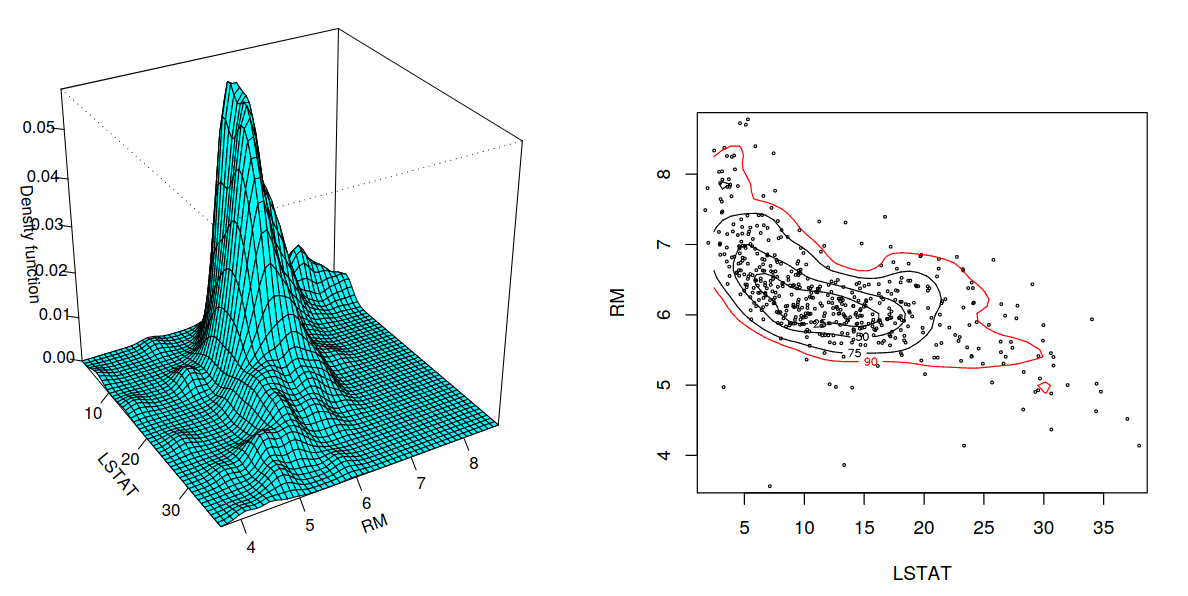
\includegraphics{figures/multivariate-kernel-density}
	\caption{Kernel estimator for the joint density function of variables
		\texttt{LSTAT} and \texttt{RM} in the \texttt{Boston} dataset.}
\end{figure}

\subsection{The curse of dimensionality}%
\label{sec:curse-of-dimensionality}%
\index{curse of dimensionality}
A general problem in multivariate non-parametric estimation, and in
particular in non-parametric density estimation, is the phenomenon
known as the curse of dimensionality:
\begin{quote}
	In high dimensional spaces the neighborhood of any point contains
	virtually no observational data.
\end{quote}

\begin{marker}
	Non-parametric estimation of the density function (or any other
	function) is extremely difficult when the data dimension $p$ is large
	(in practice $p \geq 4$).
\end{marker}

\subsection{Software}
Density estimation in R:
\begin{itemize}
	\item Functions \texttt{hist}, \texttt{density}. Bandwidth choice: \texttt{bw.nrd}, \texttt{bw.ucv},
	      \texttt{bw.bcv}, \texttt{bw.SJ}
	\item Package \texttt{KernSmooth}, functions \texttt{bkde} (for density estimation) and
	      \texttt{dpik} (for bandwidth choice). See also \texttt{dpih}. \cite{wand_kernel_1994}
	\item Package \texttt{sm}, functions \texttt{sm.density} (for density estimation) and
	      h.select (for bandwidth choice). \cite{bowman_applied_1997}
	\item Package \texttt{ks}, function \texttt{kde} for density estimation and several
	      functions for bandwidth choice. Well suited for multivariate density
	      estimation for 1- to 6-dimensional data. \cite{chacon_multivariate_2018}
\end{itemize}

\pagebreak
\section{Mixture models}
\paragraph{References:} \cite[Sections 6.8 and 12.7]{hastie_elements_2009}, \cite[Section 13.1.3]{fan_statistical_2020}, \cite[Chapter 10]{lange_numerical_1999}

\subsection{Mixture of two distributions}

The assumption that the true density function $f(\boldsymbol{x})$ follows
a \iemph{mixture model} is useful for density estimation when $p$ is \emph{large}.

\begin{definition}{Mixture Model}{mixture-model}
	\begin{equation*}
		f(\boldsymbol{x}) = \sum_{j=1}^k \alpha_j f_j(\boldsymbol{x}),\quad \alpha_j \geq 0,\quad \sum_{j=1}^k \alpha_j = 1
	\end{equation*}

	For a certain $k \geq 1$ and $p$-dimensional density functions $f_1, \dots, f_k$,
	which are assumed to be much simpler than $f(\boldsymbol{x})$.
\end{definition}

\begin{definition}{Parametric Mixture Model}{}\index{parametric mixture model}
	\begin{equation*}
		f(\boldsymbol{x}) = \sum_{j=1}^k \alpha_j f_j(\boldsymbol{x}\mid\boldsymbol{\theta}_j)
	\end{equation*}
\end{definition}

\begin{example}{Gaussian Mixture Model}{}\index{gaussian mixture model}
	\begin{equation*}
		f(\boldsymbol{x}) = \sum_{j=1}^k \alpha_j \phi(\boldsymbol{x}\mid \mu_j, \Sigma_j)
	\end{equation*}
	Where $\phi(\boldsymbol{x}\mid \mu, \Sigma)$ is the multivariate Gaussian density function
	with mean vector $\mu$ and covariance matrix $\Sigma$.
\end{example}

\begin{definition}{Model-based clustering}{}\index{model-based clustering}
	Clustering based on a parametric mixture model.
\end{definition}

\subsubsection{Mixture of two distributions (example)}

Let $(X,\,Y)$ be a bivariate random variable:
\begin{align*}
	Y               & \sim \text{Bernoulli}(p),                                               \\
	( X \mid Y = 0) & \sim f(x;\,\theta_0),                                                   \\
	( X \mid Y = 1) & \sim f(x;\,\theta_1)                                                    \\[0.5em]
	F_X(x)          & = Pr(X \leq x)                                                          \\
	                & = Pr(X \leq x \mid Y = 0) Pr(Y = 0) + Pr(X \leq x \mid Y = 1) Pr(Y = 1) \\
	                & = p F(x;\,\theta_0) + (1-p) F(x;\,\theta_1)                             \\
	                & \Downarrow                                                              \\
	f_X(x)          & = F'_X(x) = p f(x;\,\theta_0) + (1-p) f(x;\,\theta_1)
\end{align*}
$f_X(x)$ is the mixture of $f(x;\,\theta_0)$ and $f(x;\,\theta_1)$.

We observe $n$ independent observations $(x_1,\,y_1),\dots,(x_n,\,y_n)$ from $(X,\,Y)$:
\begin{alignat*}{2}
	\boldsymbol{x} & = (x_1,\,\dots,\,x_n)       & \boldsymbol{y} & = (y_1,\,\dots,\,y_n) \\
	\boldsymbol{X} & = (X_1,\,\dots,\,X_n) \quad & \boldsymbol{Y} & = (Y_1,\,\dots,\,Y_n)
\end{alignat*}

\paragraph{Likelihood function from the complete data}
\begin{align*}
	L(p,\theta_0,\theta_1;\,\boldsymbol{x},\boldsymbol{y})
	 & = \prod_{i=1}^n f(x_i \mid Y_i = y_i) Pr(Y_i = y_i)                                       \\
	 & = \prod_{i=1}^n f(x_i;\, \theta_1)^{y_i} f(x_i;\, \theta_0)^{1-y_i} p^{y_i} (1-p)^{1-y_i}
\end{align*}

The log-likelihood function is:
\begin{align*}
	\span \ell(p,\theta_0,\theta_1;\,\boldsymbol{x},\boldsymbol{y})
	= \log L(p,\theta_0,\theta_1;\,\boldsymbol{x},\boldsymbol{y})       \\
	 & = \sum_{i=1}^n \left( y_i \log p + (1 - y_i) \log(1 - p) \right)
	+ \sum_{i:y_i=1} \log f(x_i;\,\theta_1)
	+ \sum_{i:y_i=0} \log f(x_i;\,\theta_0)                             \\
	 & = \sum_{i=1}^n y_i \log \frac{p}{1-p} + n \log (1 - p)
	+ \sum_{i:y_i=1} \log f(x_i;\,\theta_1)
	+ \sum_{i:y_i=0} \log f(x_i;\,\theta_0)
\end{align*}

\subparagraph{Maximum likelihood estimation}
\begin{equation*}
	\hat{p}^{ML} = \sum_{i=1}^n \frac{y_i}{n}
\end{equation*}
For $j = 0,1$; $\hat{\theta}_j^{ML}$ is the maximum likelihood estimator of $\theta$ from the subsample
of $x_i$ corresponding to $y_i = j$.

\begin{note}
	It could be the case that $\hat{p}^{ML}$ can be calculated using a closed-form solution
	(e.g. Mixture of two Gaussians). But even if it is not the case, the optimization
	problem is easier than direct maximization with respect to $p,\theta_0,\theta_1$.
\end{note}

\paragraph{Likelihood function from the incomplete data}

If we only observe data from $X$ the likelihood function is:
\begin{align*}
	L(p,\theta_0,\theta_1;\,\boldsymbol x)    & = \prod_{i=1}^n f_X(x_i)                                                         \\
	                                          & = \prod_{i=1}^n \left( p f(x_i;\,\theta_1) + (1-p) f(x_i;\,\theta_0) \right)     \\[1em]
	\ell(p,\theta_0,\theta_1;\,\boldsymbol x) & = \sum_{i=1}^n \log \left( p f(x_i;\,\theta_1) + (1-p) f(x_i;\,\theta_0) \right)
\end{align*}

In this case, the MLE involves ($p,\theta_0,\theta_1$) jointly.
And \emph{very rarely} we can find a closed-form solution for the MLE.

Unfortunately, the standard situation is that the data is incomplete
(the indicator variables $Y_1,\dots,Y_n$ are not observed).

\begin{question}{Can we have an optimization problem similar to that of the complete data
		$(X,\,Y)$ even if we observe only the incomplete data $X$?}{}
	Yes, we can use the EM algorithm.
\end{question}

\subsection{The EM algorithm}\index{EM algorithm}

Since the complete data log-likelihood $\ell(p,\theta_0,\theta_1;\,\boldsymbol{X},\boldsymbol{Y})$
cannot be computed when only incomplete
data $\boldsymbol{X}$ is observed, we maximize its conditional expectation given
$\boldsymbol{X} = \boldsymbol{x}$ instead:
\begin{align*}
	E \left(\ell(p,\theta_0,\theta_1;\,\boldsymbol{X},\boldsymbol{Y}) \mid \boldsymbol{X}=\boldsymbol{x} \right)
	= & \sum_{i=1}^n E(Y_i \mid \boldsymbol{X}=\boldsymbol{x}) \log \frac{p}{1-p} + n \log (1 - p) \\
	  & + \sum_{i=1}^n E(Y_i \mid \boldsymbol{X}=\boldsymbol{x}) \log f(x_i;\,\theta_1)            \\
	  & + \sum_{i=1}^n (1 - E(Y_i \mid \boldsymbol{X}=\boldsymbol{x})) \log f(x_i;\,\theta_0)
\end{align*}

\subsubsection{The E(xpectation)-step}
$(Y_i \mid \boldsymbol{X}=\boldsymbol{x})$ is a Bernoulli random variable with parameter
$p = P(Y_i = 1 \mid \boldsymbol{X}=\boldsymbol{x})$. Thus, by Bayes' theorem:
\begin{align*}
    E(Y_i \mid \boldsymbol{X}=\boldsymbol{x}) & = P(Y_i = 1 \mid \boldsymbol{X}=\boldsymbol{x})
    \propto f_{\boldsymbol{X}}(\boldsymbol{x} \mid Y_i = 1) P(Y_i = 1) \\
                                              &= \prod_{h=1}^n f_{X_h}(x_h \mid Y_i = 1) P(Y_i = 1)
                                              \propto f_X(x_i \mid Y_i = 1) P(Y_i = 1) = f_X(x_i;\,\theta_1) p
\end{align*}
Analogously: $P(Y_i = 0 \mid \boldsymbol{X}=\boldsymbol{x}) = f_X(x_i;\,\theta_0) (1-p)$.

Using that $P(Y_i = 1 \mid \boldsymbol{X}=\boldsymbol{x}) + P(Y_i = 0 \mid \boldsymbol{X}=\boldsymbol{x}) = 1$,
and assuming that $p, \theta_0, \theta_1$ are known:
\begin{align*}
    P(Y_i = 1 \mid \boldsymbol{X}=\boldsymbol{x}) & = \frac{f_X(x_i;\,\theta_1) p}{f_X(x_i;\,\theta_1) p + f_X(x_i;\,\theta_0) (1-p)} \tag{$\hat{y}_i$}\\
    P(Y_i = 0 \mid \boldsymbol{X}=\boldsymbol{x}) & = \frac{f_X(x_i;\,\theta_0) (1-p)}{f_X(x_i;\,\theta_1) p + f_X(x_i;\,\theta_0) (1-p)}
\end{align*}

Let
\begin{align*}
    \hat{y}_i & = E(Y_i \mid \boldsymbol{X}=\boldsymbol{x}) ) =
    P(Y_i = 1 \mid \boldsymbol{X}=\boldsymbol{x}) \\
              &= \frac{f_X(x_i;\,\theta_1) p}{f_X(x_i;\,\theta_1) p + f_X(x_i;\,\theta_0) (1-p)}
              = \hat{y}_i(p,\theta_0,\theta_1)
\end{align*}

\subsubsection{The M(aximization)-step}
We want to maximize the conditional expectation of the log-likelihood function:
\begin{align*}
    E \left(\ell(p,\theta_0,\theta_1;\,\boldsymbol{X},\boldsymbol{Y}) \mid \boldsymbol{X}=\boldsymbol{x} \right)
    = & \left(
        \sum_{i=1}^n \hat{y}_i \log \frac{p}{1-p} + n \log (1 - p)
        \right) \\
      & + \sum_{i=1}^n \hat{y}_i \log f(x_i;\,\theta_1) + \sum_{i=1}^n (1 - \hat{y}_i) \log f(x_i;\,\theta_0)
\end{align*}

If we consider $\hat{y}_i$ as fixed (ignoring its dependence on $p, \theta_0, \theta_1$), the
previous function is the sum of 3 functions, each depending on a single parameter:
\begin{alignat*}{2}
    \max_{p}&\left( \sum_{i=1}^n \hat{y}_i \log \frac{p}{1-p} + n \log (1 - p) \right) & \quad \rightarrow{} \quad
    \hat{p} & = \frac{\sum_{i=1}^n \hat{y}_i}{n} \\
    \max_{\theta_1}&\sum_{i=1}^n \hat{y}_i \log f(x_i;\,\theta_1) \\
    \max_{\theta_0}&\sum_{i=1}^n \hat{y}_i \log f(x_i;\,\theta_0)
\end{alignat*}

$\hat{\theta}_1$ and $\hat{\theta}_0$ are the weighted maximum likelihood estimates
of $\theta$ with weights $\hat{y}_i$ and $1 - \hat{y}_i$, respectively.

\begin{marker}
    The \emph{EM-algorithm} consists of iterating the E-step and the M-step until convergence.
\end{marker}

\subsection{Software}
\begin{itemize}
	\item Package \texttt{ClusterR}
	      \begin{itemize}
		      \item \texttt{GMM}: fits a Gaussian mixture model to the data using the EM algorithm.
		      \item \texttt{Optimal\_Clusters\_GMM} to determine the optimal number of clusters.
		      \item Also includes other clustering methods such as $k$-means and $k$-medoids.
	      \end{itemize}
	\item Package \texttt{mclust}: model-based clustering, classification and density estimation
        based on finite normal mixture modeling.
	      \begin{itemize}
		      \item \texttt{Mclust}: Model-based clustering based on parameterized finite
                  Gaussian mixture models. Modesl are estimated by EM algorithm. The optimal
                  model is selected by \iemph{BIC} (Bayesian Information Criterion).
	      \end{itemize}
	\item Package \texttt{fpc}, Flexible Procedures for Clustering:
	      \begin{itemize}
		      \item \texttt{mergenormals}: Clustering by merging components of a Gaussian mixture.
		      \item \texttt{cluster.stats}: Computes several cluster validity statistics from a
		            clustering and a dissimilarity matrix.
	      \end{itemize}
\end{itemize}

\pagebreak
\section{Density based clustering}
\paragraph{References:} \cite{ester_density-based_1996}
\subsection{DBSCAN}

Density-Based Spatial Clustering of Applications with Noise (DBSCAN) is
a density-based clustering algorithm that is able to find clusters of
arbitrary shape.

\begin{definition}{Density-based clusters}{}\index{density-based clusters}
	Connected areas of the sample space with high \emph{density of observations}.
\end{definition}

\begin{definition}{Outliers (noise)}{}
	Observed points that are not part of any cluster.
\end{definition}

\subsection{Measuring the density of observations}
Let $\mathcal{D} = \{ \boldsymbol{x}_1, \ldots, \boldsymbol{x}_n \}$ be a set of $n$ observations
in a $p$-dimensional space. For each observation $\boldsymbol{x}_i$, we define the $\varepsilon-$\iemph{neighborhood}
of $\boldsymbol{x}_i$ as the set of points $\boldsymbol{x}_j$ such that:
\begin{equation*}
    N_{\varepsilon}(\boldsymbol{x}_i) = \bigl\{
    \boldsymbol{x}_j \in \mathcal{D} \mid d(\boldsymbol{x}_i,\,\boldsymbol{x}_j) \leq \varepsilon
    \bigr\}
\end{equation*}
where $d(\boldsymbol{x}_i,\,\boldsymbol{x}_j)$ is a distance measure between points in $\mathds{R}^p$.

The \iemph{density of observations} around $\boldsymbol{x}_i$ is estimated by the number
of observations at $N_{\varepsilon}(\boldsymbol{x}_i)$.

Observe that this is proportional to:
\begin{equation*}
    \hat{f}_\varepsilon(\boldsymbol{x}_i) =
    \frac{|N_{\varepsilon}(\boldsymbol{x}_i)| / n}{\text{Volume}(N_{\varepsilon}(\boldsymbol{x}_i))}
    = \frac{|N_{\varepsilon}(\boldsymbol{x}_i)| / n}{\text{Volume}(\varepsilon^p N_{1}(\boldsymbol{0}))}
\end{equation*}
which is the kernel estimator of the probability density function at $\boldsymbol{x}_i$
when using an uniform kernel on $\mathds{R}^p$ and bandwidth of $\varepsilon$.

\subsubsection{Main concepts}
\begin{definition}{Core point}{}\index{core point}
    A point $\boldsymbol{x}_i$ is a \emph{core point} if $|N_{\varepsilon}(\boldsymbol{x}_i)| \geq \text{minPts}$.

    That is, if the estimated density of observations around $\boldsymbol{x}_i$ is over a certain threshold.
\end{definition}

\begin{definition}{Border point}{}\index{border point}
    A point $\boldsymbol{x}_i$ is a \emph{border point} if it is not a core point but it is
    in the $\varepsilon-$neighborhood of a core point.
\end{definition}

\begin{definition}{Noise point (or outlier)}{}\index{noise point}
    A point $\boldsymbol{x}_i$ is a \emph{noise point} if it is not a core point and it is not a border point.
\end{definition}

\begin{definition}{Densly connected}{}\index{densly connected}
    Two points $\boldsymbol{x}_0$ and $\boldsymbol{x}_{m+1}$ are \emph{densly connected} if
    there is a path of \emph{core points} $\boldsymbol{x}_1, \ldots, \boldsymbol{x}_{m}$ such
    that $d(\boldsymbol{x}_i,\,\boldsymbol{x}_{i+1}) \leq \varepsilon$ for all $i = 0, \ldots, m$.

    \tcblower
    Observe that $\boldsymbol{x}_0$ and/or $\boldsymbol{x}_{m+1}$ can be core or border points.
\end{definition}

\begin{definition}{Cluster}{}\index{cluster}
    
    Clusters are subsets of density-connected points (all the points in the cluster are
    density-connected) which are maximal (if a point $\boldsymbol{x}_i$ is density-connected
    with another point $\boldsymbol{x}_j$, then both points are in the same cluster).

    \tcblower

    Only core and border points can be part of a cluster.

    Outliers are not part of any cluster.

    The number of clusters is not known in advance.

    The core points in a DBSCAN cluster are a subset of observed points belonging to the same
    connected component of the level set of the estimated density function:
    \begin{equation*}
        \left\{
            \boldsymbol x \in \mathds{R}^p \mid \hat{f}_\varepsilon(\boldsymbol x) \geq f_0
        \right\}
    \end{equation*}
    where the threshold $f_0$ is: $\frac{\text{minPts}}{n \cdot \varepsilon^p \text{Volume}(N_{1}(\boldsymbol{0}))}$.
    
\end{definition}

\begin{algorithm}{DBSCAN}{}
    \begin{algorithmic}[1]
    \Procedure{DBSCAN}{$\varepsilon$, minPts}
        \State Mark each point $\boldsymbol{x}_i$ as either core, border or noise
        \State Remove all noise points
        \State $j \gets 0$
        \While{There are still core points}
            \State Select a random core point $\boldsymbol{x}_i$
            \State Define a new cluster $C_j$ with $\boldsymbol{x}_i$
            \State Add to $C_j$ all points density-connected to $\boldsymbol{x}_i$
            \State Add to $C_j$ all border points density-connected to $\boldsymbol{x}_i$
            \State Remove all points in $C_j$ from the set of core points
            \State $j \gets j + 1$
        \EndWhile
    \EndProcedure
\end{algorithmic}
\tcblower
\begin{marker}
There are two hyperparameters in DBSCAN: $\varepsilon$ and $\text{minPts}$.
\end{marker}
\end{algorithm}

\begin{figure}[H]
    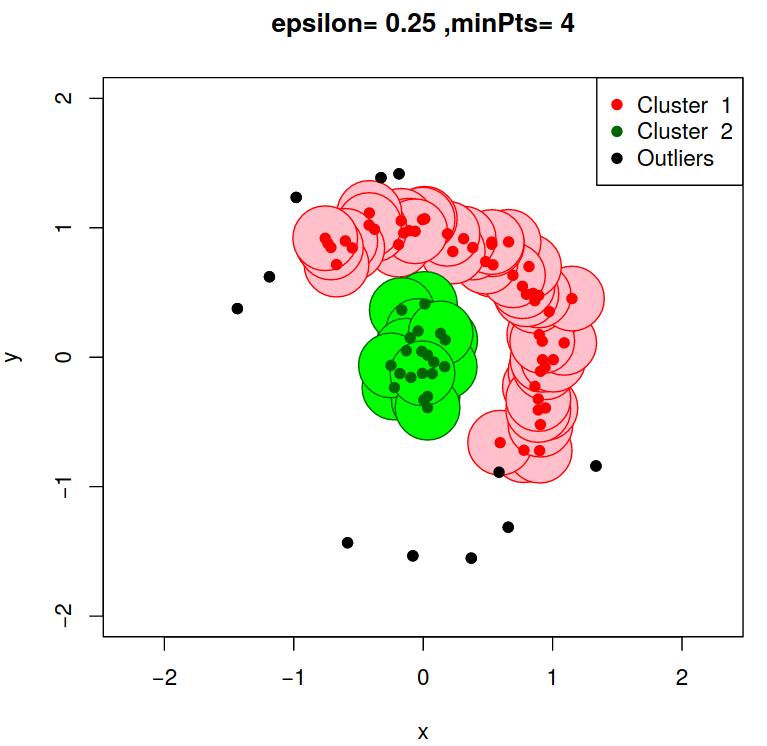
\includegraphics[width=0.6\textwidth]{../figures/dbscan_eps_minpts}
    \caption{Visualization of the DBSCAN algorithm}
\end{figure}

\subsection{Software}

\begin{itemize}
	\item Package \texttt{fpc}, Flexible Procedures for Clustering:
	      \begin{itemize}
		      \item \texttt{dbscan}: Computes DBSCAN density based clustering as introduced
		            in \cite{ester_density-based_1996}.
		      \item \texttt{cluster.stats}: Computes several cluster validity statistics from a
		            clustering and a dissimilarity matrix.
	      \end{itemize}
	\item Package \texttt{dbscan}, function \texttt{dbscan}: Fast reimplementation of the
	      DBSCAN.
\end{itemize}

%! TEX root = ../000-main.tex
\chapter{Nonlinear dimensionality reduction}
\chaptermark{NL dim. red.}

\section[Introduction]{Introduction to dimensionality reduction}
\paragraph{References:}
\cite[Chapter 8]{johnson_applied_2007},
\cite[Chapters 5 and 6]{pena_alisis_2002},
\cite[Section 11.1]{venables_exploratory_2002},
\cite[Sections 14.5.1, 14.8 and 14.9]{hastie_elements_2009}

We observe $n$ independent objects $\mathcal{O}_i,\;i=1,\ldots,n$ from a given population.

In general, they belong to a large-dimensional (or even infinite-dimensional) space $\Omega$.

\begin{problem}{Dimensionality reduction problem}{}
We want to find a low dimensional configuration $\boldsymbol{Y}$, that is an
$n \times q$ matrix, where $q < n$ such that each of its rows $\boldsymbol{y}_i$ can
be identified with the observed object $\mathcal{O}_i$ in some way:
\begin{itemize}
	\item An application $\rho: \mathbb{R}^q \to \Omega$ such that
	      $\rho(\boldsymbol{y}_i) \approxeq \mathcal{O}_i,\quad i=1,\ldots,n$.
	\item We can define a distance between $\boldsymbol{y}_i$ and $\boldsymbol{y}_j$,
	      such that the distance between $\mathcal{O}_i$ and $\mathcal{O}_j$ is close
	      to the dissimilarity between the observed objects $\mathcal{O}_i$ and
	      $\mathcal{O}_j,\; \forall i,j \in \{1,\ldots,n\}$.
	\item \ldots
\end{itemize}
\begin{note}
	When dimensionality reduction is for visualization purposes, $q = 2$ is
	usually chosen.
\end{note}
\end{problem}

\subsection{Two types of information from the observed objects}
We consider two different ways of extracting information from the observed objects:
\begin{itemize}
	\item Sampling information as a \iemph{data matrix} $\boldsymbol{X}$ of
	      size $n \times p$ ($n$ individuals and $p$ attributes, $p \gg q$).
	      \begin{itemize}
		      \item Principal component analysis (PCA).
		      \item Principal curves (Nonlinear version of PCA) \cite{hastie_principal_1989,delicado_another_2001}.
	      \end{itemize}
	\item Sampling information as a distance matrix $\boldsymbol{D}$ of size
	      $n \times n$.
	      \begin{itemize}
		      \item Multidimensional scaling (MDS).
		      \item Local MDS
		      \item Isometric mapping (ISOMAP, Nonlinear version of MDS).
		      \item t-Stochastic Neighbor Embedding (t-SNE).
	      \end{itemize}
\end{itemize}

\section[Principal Component Analysis]{Principal Component Analysis (PCA)}\index{PCA}

\begin{definition}{Principal component analysis (PCA)}{PCA}
	Multivariate analysis technique that intends to explain the
	\iemph{variance-covariance structure} through a few linear combinations of the original
	variables.

	\paragraph{Main goals:} Interpretation and dimensionality reduction.
\end{definition}

\begin{definition}{Variance-covariance structure}{}
	The variance-covariance structure of a random vector $\boldsymbol{X} \in \mathbb{R}^p$
	is defined as the $p \times p$ matrix $\boldsymbol{V} = \boldsymbol{V}(\boldsymbol{X})$
	such that:
	\begin{equation*}
		\boldsymbol{V}_{ij} = \mathrm{Cov}(X_i,X_j) = \mathrm{E}[(X_i - \mathrm{E}[X_i])(X_j - \mathrm{E}[X_j])].
	\end{equation*}
	\tcblower
	The variance is the diagonal of the variance-covariance matrix:
	\begin{equation*}
		\boldsymbol{\sigma}^2 = \mathrm{diag}(\boldsymbol{V}).
	\end{equation*}
\end{definition}

\subsubsection{Finding the first principal component (q=1)}
\begin{figure}[H]
	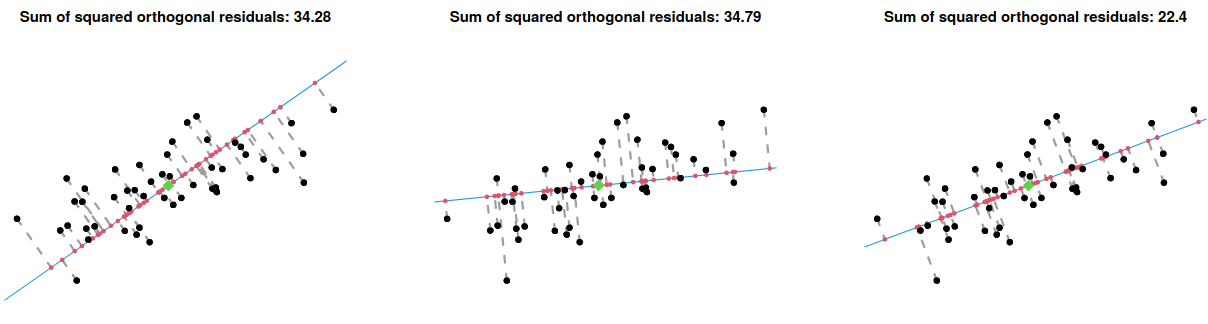
\includegraphics{pca_q1}
\end{figure}
We observe $\boldsymbol{x}_i \in \mathbb{R}^p,\;i=1,\ldots,n$ with mean $\boldsymbol{m}$.
For $\boldsymbol{a} \in \mathbb{R}^p,\, \lVert \boldsymbol a \rVert = 1$, the
projection vector of $(\boldsymbol{x} - \boldsymbol{m})$ in the direction of $\boldsymbol{a}$ is:
$P_{\boldsymbol{a}}(\boldsymbol{x} - \boldsymbol{m}) = \bigl( (\boldsymbol x - \boldsymbol m)' \boldsymbol a \bigr)
	\boldsymbol{a}$. These two problems:
\begin{align*}
	\min_{\boldsymbol{a} \in \mathbb{R}^p,\, \lVert \boldsymbol a \rVert = 1} & \sum_{i=1}^n
	\left\lVert \boldsymbol{x}_i - \boldsymbol{m} - P_{\boldsymbol{a}}(\boldsymbol{x}_i - \boldsymbol{m}) \right\rVert^2 \tag{Minimizing the orthogonal residuals} \\
	\max_{\boldsymbol{a} \in \mathbb{R}^p,\, \lVert \boldsymbol a \rVert = 1} & \sum_{i=1}^n
	\left\lVert P_{\boldsymbol{a}}(\boldsymbol{x}_i - \boldsymbol{m}) \right\rVert^2
	\tag{Maximizing the inertia of the projected data}
\end{align*}
have the same solution $\boldsymbol{a}^*$, which we will call the \iemph{first principal component},
by Pythagoras' theorem:
\begin{equation*}
	\sum_{i=1}^n \left\lVert \boldsymbol{x}_i - \boldsymbol{m} \right\rVert^2
	= \sum_{i=1}^n \left\lVert
	\boldsymbol{x}_i - \boldsymbol{m} - P_{\boldsymbol{a}^*}(\boldsymbol{x}_i - \boldsymbol{m})
	\right\rVert^2
	+ \sum_{i=1}^n \left\lVert P_{\boldsymbol{a}^*}(\boldsymbol{x}_i - \boldsymbol{m}) \right\rVert^2.
\end{equation*}

Let $\hat{V} = (\boldsymbol{v}_1,\ldots,\boldsymbol{v}_p)$ and $\hat{D} = \mathrm{Diag}(\hat{\lambda}_1,\ldots,\hat{\lambda}_p)$

Let $\boldsymbol S = \hat{V}\hat{D}\hat{V}'$ be the spectral decomposition of $\boldsymbol{S}$.

Then, the data matrix of sampling principal components is:
\begin{equation*}
	\boldsymbol{Y} = (\boldsymbol{y}_1,\ldots,\boldsymbol{y}_n) = (\boldsymbol{X} - \boldsymbol 1_n \boldsymbol m ')\hat{V}.
\end{equation*}
Roughly speaking, the sampling principal components are uncorrelated linear combinations of the
observed variables having the largest possible variability.

\begin{note}
	In this, way one of the two main goals of PCA is met: Interpretation.
\end{note}

\subsection{Single value decomposition (SVD)}

\begin{theorem}{Singular-Value Decomposition}{svd}
	Let $A$ be an $n \times p$ matrix. Then there exists an orthogonal matrix $U$ of size $n \times n$,
	and a orthogonal matrix $V$ of size $p \times p$ such that:
	\begin{equation*}
		A = U \Gamma V'
	\end{equation*}
	Where the $n \times p$ matrix $\Gamma$ has $(i,\, i)$ entry $\gamma_i \geq 0,\;i=1,\ldots,\min(n,p)$
	and the other entries are zero (diagonal matrix). The positive entries $\gamma_i$ are called
	the \iemph{singular values} of $A$. The number of singular values coincides with $k$, the rank of $A$.
	\tcblower
	\paragraph{Remark:} Let $\boldsymbol{u}_i$ be the columns of $U$ and let $\boldsymbol{v}_i'$ be the
	rows of $V'$. Then:
	\begin{equation*}
		A = U \Gamma V' = \sum_{i=1}^k \gamma_i \boldsymbol{u}_i \boldsymbol{v}_i'
	\end{equation*}
\end{theorem}

\subsubsection{SVD and PCA}

Let $A = \boldsymbol{X} - \boldsymbol 1_n \boldsymbol m '$. Then $A'A = (n - 1) \boldsymbol{S} =
	(n - 1) \hat{V} \hat{D} \hat{V}'$.

Let $(\boldsymbol X - \boldsymbol 1_n \boldsymbol m ') = \hat{U}\Gamma \hat{V}'$ be SVD of $A$

$\boldsymbol{Y} = (\boldsymbol X - \boldsymbol 1_n \boldsymbol m ') \hat{V} \iff
	\boldsymbol Y \hat{V}' = (\boldsymbol X - \boldsymbol 1_n \boldsymbol m ') = \hat{U}\Gamma\hat{V}'$,
then $\boldsymbol{Y} = \hat{U}\Gamma$.

The best approximation of rank $s$ to $A$ is:
\begin{equation*}
	\sum_{j=1}^s \gamma_j \boldsymbol{u}_j \boldsymbol{v}_j' = \sum_{j=1}^s \boldsymbol{y}_j \boldsymbol{v}_j'
\end{equation*}
Therefore, the best approximation to $\boldsymbol{X}$ of rank $s$ is:
\begin{equation*}
	\boldsymbol{X} \approx \boldsymbol 1_n \boldsymbol m ' + \sum_{j=1}^s \boldsymbol{y}_j \boldsymbol{v}_j'
\end{equation*}
For the $i$-th row of $\boldsymbol{X}$:
\begin{equation*}
	\boldsymbol{x}_i \approx \boldsymbol{m} + \sum_{j=1}^s y_{ij} \boldsymbol{v}_j'
\end{equation*}
where $y_{ij}$ is the score of the $i$-th observation on the $j$-th principal component.

\begin{note}
	With this, the second goal of PCA is met: Dimensionality reduction.
\end{note}

\section{Multidimensional scaling (MDS)}

\begin{definition}{Multidimensional scaling (MDS)}{mds}\index{mds}
	is a dimensionality reduction technique based on \emph{inter-individual distances}.
\end{definition}

\begin{definition}{Euclidean configuration}{}
	For $n$ individuals, let $\boldsymbol{D} = (\delta_{ij})$ be the $n \times n$ matrix of inter-individual
	distances.

	Assume that for a $q \leq n$ there exists a $n \times q$ data matrix $\boldsymbol{X}$ such that
	the Euclidean distance between the $i$-th and $j$-th row of $\boldsymbol{X}$,
	$\left\lVert \boldsymbol{x}_i - \boldsymbol{x}_j \right\rVert$, is equal to $\delta_{ij}$.

	We say that $\boldsymbol{X}$ is a \iemph{Euclidean configuration} of $\boldsymbol{D}$.
	\tcblower
	\begin{note}
		Such configuration does not always exist.
	\end{note}
\end{definition}

\begin{definition}{Principal coordinates}
When it does exist, $\boldsymbol{D}$ is said to be Euclidean. In this
case $\boldsymbol{X}$ can be chosen verifying the following conditions:
\begin{itemize}
	\item It has orthogonal columns.
	\item For $1 \leq q \leq r$, the first $q$ columns of $\boldsymbol{X}$,
	      $\boldsymbol{\tilde{X}}_a$, make up the $q$-dimensional configuration that
	      best approximates the observed distances.
\end{itemize}
The columns of $\boldsymbol{X}$ are called \iemph{principal coordinates}.

\tcblower

\begin{note}
When an Euclidean configuration does not exist, MDS allows to
obtain \emph{approximated solution}s.

That is, MDS looks for a $q$-dimensional
configuration $\boldsymbol{X}$ such that the Euclidean distances between
the rows of $\boldsymbol{X}$ are \emph{as close as possible} to the observed
distances.
\end{note}
\end{definition}


\subsection{Classical metric scaling}

If a $n \times p$ matrix $\boldsymbol{X}$ (with 0 mean by columns) is observed
and Euclidean distances are used, then: \emph{MDS and PCA give the same results}.

\subsection{Non-classical metric scaling}%
\label{sec:non-classical-metric-scaling}

Let $\boldsymbol{D} = (\delta_{ij})^n_{i,j=1}$ be the inter-individual distance
matrix recorded for the $n$ objects forming our sample.

Fix a tentative dimension $q$ and a $n \times q$ matrix $\boldsymbol{X}$.
Let $d_{ij} = \left\lVert \boldsymbol{x}_i - \boldsymbol{x}_j \right\rVert$ be the
Euclidean distance between the $i$-th and $j$-th row of $\boldsymbol{X}$.

The metric \iemph{STRESS} (STandardized REsidual Sum of Squares), a measure
of the relative error made when matrix $\boldsymbol{X}$ is considered as
an Euclidean configuration for the distance matrix $\boldsymbol{D}$, is defined as:
\begin{equation*}
	\text{STRESS}_M(\boldsymbol{D},\, \boldsymbol{X}) = \sqrt{\frac
		{\sum_{i<j}(\delta_{ij} - d_{ij})^2}
		{\sum_{i<j}\delta_{ij}^2}
	}
\end{equation*}

\begin{problem}{Non-classical metric scaling}{}
\begin{equation*}
	\min_{\boldsymbol{X} \in \mathds{R}^{n\times q}} \text{STRESS}_M(\boldsymbol{D},\, \boldsymbol{X})
\end{equation*}
\end{problem}

There is also S-STRESS:
\begin{equation*}
	\text{S-STRESS}_M(\boldsymbol{D}, \boldsymbol{X}) = \sqrt{\frac
		{\sum_{i<j}(\delta_{ij}^2 - d_{ij}^2)^2}
		{\sum_{i<j}\delta_{ij}^4}
	}
\end{equation*}

\subsection{Non-metric scaling}
Non-metric scaling uses only the ranks of the inter-individual distances $\delta_{ij}$.
The metric used is the Non-metric Stress (NMS):
\begin{equation*}
	\text{STRESS}_{NM}(\boldsymbol{D},\, \boldsymbol{X},\, f) = \sqrt{\frac
	{\sum_{i<j}(\text{rank}(\delta_{ij}) - d_{ij})^2}
	{\sum_{i<j}d_{ij}^2}
	}
\end{equation*}
Where $f: \mathds{R}^+ \to \mathds{R}^+$ is an increasing function.

\begin{problem}{Non-metric scaling}{}
\begin{equation*}
    \mathlarger{\min_{\boldsymbol{X} \in \mathds{R}^{n\times q}}} \min_{f\uparrow} \text{STRESS}_{NM}(\boldsymbol{D},\, \boldsymbol{X},\, f)
\end{equation*}
\end{problem}

\section{Distances and similarities}

\begin{definition}{Metric and Semi-metric}{metric}

	Let $\Omega$ be a set of objects. The application:
	\begin{equation*}
		d: \Omega \times \Omega \to \mathds{R}
	\end{equation*}
	is a \iemph{semi-metric} if it verifies the following properties $\forall P, Q, R \in \Omega$:
	\begin{align*}
		d(P, Q) & = d(Q, P) \tag{symmetry}                         \\
		d(P, Q) & \geq 0 \tag{non-negativity}                      \\
		d(P, P) & = 0 \tag{identity}                               \\
		d(P, Q) & \leq d(P, R) + d(R, Q) \tag{triangle inequality}
	\end{align*}

	\begin{marker}
		Additionally, if $d(P, Q) = 0 \implies P = Q$, then $d$ is a \iemph{metric} (or \emph{distance}).
	\end{marker}
\end{definition}

\begin{definition}{Similarity}{similarity}

	Let $\Omega$ be a set of objects. The application:
	\begin{equation*}
		s: \Omega \times \Omega \to \mathds{R}
	\end{equation*}
	is a \iemph{similarity} if it verifies the following properties $\forall P, Q, R \in \Omega$:
	\begin{align*}
		s(P, Q) & = s(Q, P) \tag{symmetry}    \\
		s(P, Q) & \geq 0 \tag{non-negativity} \\
		s(P, P) & = s(Q, Q)                   \\
		s(P, Q) & \leq s(R, R)
	\end{align*}
	Additionally, it is required that $s(P, Q)$ is an increasing function of
	the proximity between $P$ and $Q$.
\end{definition}

\subsection{Similarities to and from distances}
\begin{equation*}
	s(P, Q) = \frac{1}{1 + d(P, Q)}
\end{equation*}

If the similarity function $s$ is a valid kernel function with $s(P, P) = 1,\;\forall P\in\Omega$,
and $s(P, Q) < 1,\;\forall P \neq Q \in \Omega$, then:
\begin{equation*}
	d(P, Q) = \sqrt{2\bigl(1 - s(P, Q)\bigr)}
\end{equation*}

\clearpage
\section{Principal Curves}

\subsection{Introduction}

\begin{definition}{First principal component}{}
	The straight line fitting best a data cloud.
\end{definition}

\begin{problem}{Principal curves}{}
Given a dataset with a non-elliptical configuration,
look for the curve best fitting the data.
\end{problem}

\begin{definition}{Principal curves}{}
	Smooth one-dimensional curves that pass through the middle of a
	$p$-dimensional data set, providing a non-linear summary of the data.
	\cite{hastie_principal_1989}
	\tcblower
	\begin{note}
		Principal curves are \emph{non-linear} and \emph{non-parametric} generalizations
		of the first principal component.
	\end{note}
\end{definition}

\subsection{Dimensionality reduction by a curve}
We observe $n$ independent objects $\mathcal{O}_i = \boldsymbol{x}_i,\, i = 1, \dots, n$ from
a r.v.%
\footnote{Random variable}
$\boldsymbol{X}$ with values in the large dimensional space $\Omega = \mathds{R}^p$.
\begin{problem}{Dimensionality reduction by a curve}{}
Looking for a \emph{one-dimensional} configuration $\boldsymbol{y} \in \mathds{R}^n$ such
that each value $y_i$ of $\boldsymbol{y}$ can be identified with the observed
$\boldsymbol{x}_i$ in the following way:

There exists a one-dimensional differentiable parametric function $\alpha$ from
$[a, b] \subseteq \mathds{R} \to \mathds{R}^p$ whose image:
\begin{equation*}
	\left\{ \boldsymbol{x} \in \mathds{R}^p \mid \boldsymbol{x} = \alpha(y), \, y \in [a, b]  \right\}
\end{equation*}
is called a \iemph{curve}, such that $\alpha(y_i)$ is close to the observed $\boldsymbol{x}_i$ for
all $i = 1, \dots, n$.
\tcblower
\begin{note}
	The function $\alpha : \mathds{R} \to \mathds{R}^p$ is also called a \emph{curve}.
\end{note}
\begin{note}
	For dimension $q$, $1 < q < p$, the concept of \iemph{manifold} $\rho: \mathds{R}^q \to \mathds{R}^p$
	extends that of curve to a $q$-dimensional space.
\end{note}
\end{problem}

\subsection{Principal curves according to Hastie and Stuetzle}

The first definition of principal curves was given by Hastie and Stuetzle in \cite{hastie_principal_1989}.
It does not include parametric assumptions.

The definition is based on the concept of \emph{self-consistency}:
\begin{definition}{HSPC}{}
	A curve $\alpha$ is a \iemph{Hastie-Stuetzle principal curve} if it is self-consistent.
\end{definition}

\begin{definition}{Self-consistency (curves)}{}
	A curve $\alpha$ is \iemph{self-consistent} if for all $\alpha(s)$ in the curve,
	this point is the conditional mean of $\boldsymbol X$ given that $\boldsymbol X$ belongs
	to the attraction domain of $\alpha(s)$.
\end{definition}

\begin{definition}{Domain of attraction of a point of $\alpha(s)$}{}

	The domain of attraction of a point $\alpha(s)$ in a differentiable curve $\alpha$
	is, usually, the orthogonal hyperplane to $\alpha$ at $\alpha(s)$:
	\begin{equation*}
		H(\alpha(s), \alpha'(s)) = \left\{
		\boldsymbol{y} \in \mathds{R}^p \mid \boldsymbol{y} - \alpha(s) \perp \alpha'(s)
		\right\}
	\end{equation*}
	Where $\alpha'(s)$ is the \iemph{velocity vector} to $\alpha$ at $s$, which is
	the component-wise derivative of $\alpha$ and it is tangent to $\alpha$ at $\alpha(s)$.
\end{definition}

\begin{figure}[H]
	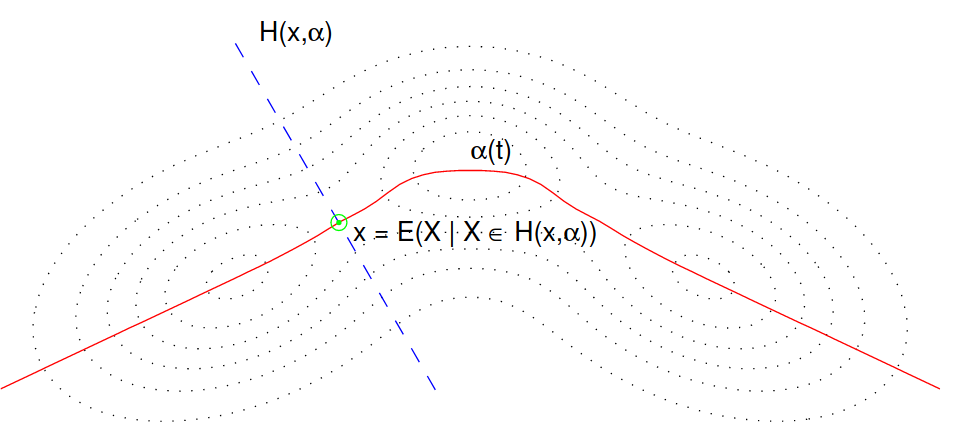
\includegraphics{hspc}
	\caption{Hastie-Stuetzle principal curve}
\end{figure}

\subsubsection{Theoretical drawbacks of HSPCs}

\begin{itemize}
	\item Neither existence nor uniqueness of HSPCs is guaranteed.
	\item Let $S$ be a r.v. in $\mathds{R}$, let $\alpha: \mathds{R} \to \mathds{R}^p$, let $\varepsilon$
	      be a zero-mean r.v. in $\mathds{R}^p$, $S$ and $\varepsilon$ are independent. Define
	      $\boldsymbol{X} = \alpha(S) + \varepsilon$. Then, in general, the
	      generating curve $\alpha$ is not a HSPC of $\boldsymbol{X}$.
	\item For a $p$-dimensional normal distribution, all the principal components are HSPC. Which
	      means that HSPC are generalizing a property that does not characterize uniquely the first
	      principal component.
\end{itemize}

\subsubsection{Theoretical algorithm for HSPC}

The algorithm proposed by Hastie and Stutzle to find the principal curve
consists of the iteration until convergence of the function $\mathcal W_{\boldsymbol X}$:
\begin{equation*}
	\alpha_{k+1} = \mathcal W_{\boldsymbol X}(\alpha_k) =
	\left\{
	\boldsymbol x \in \mathds{R}^p : \boldsymbol x = \mathds{E}(\boldsymbol X \mid \boldsymbol X \in
	D_{\alpha_k}(\boldsymbol y)) \mid \text{for some }\boldsymbol y \in \alpha_k
	\right\}
\end{equation*}
that is, for any $s \in [a, b] \subseteq \mathds{R}$:
\begin{equation*}
	\alpha_{k+1}(s) = \mathds{E}(\boldsymbol X \mid \boldsymbol X \in H(\alpha_k(s),\, \alpha_k'(s)))
\end{equation*}
with the first principal component (PC1) line as initial set $\alpha_0$.

\paragraph{Practical computation}
In practice, populational concepts are replaced by sampling ones:
\begin{itemize}
	\item PC1 is replaced by the set of the projected observed points on the line:
	      \begin{equation*}
		      \alpha_0 = \left\{
		      \boldsymbol y_i = \boldsymbol{\overline{x}}_n + s_i \boldsymbol{v}_1 \mid i = 1, \dots, n
		      \right\}
	      \end{equation*}
	      Where $\boldsymbol{\overline{x}}_n$ is the sample mean of the observed points and, $\boldsymbol{v}_1$
	      is the direction of the first principal component and $s_i$ are the scores of the observed
	      data on PC1.
	\item Numerical derivation is used to compute the velocity vector $\alpha_k'(s_i)$.
	\item Smoothing methods are used to estimate the conditional expectations
	      $\mathds{E}(\boldsymbol X \mid \boldsymbol X \in H(\alpha_k(s),\, \alpha_k'(s)))$.
\end{itemize}
\begin{note}
	The algorithm that computes HSPC is implemented in the \texttt{princurve} package in R.
\end{note}

\subsection{Principal curves of oriented points}

Delicado \cite{delicado_another_2001} propeses to generalize the following property of the
first principal component (the straight line
$\{\mathds{E}(\boldsymbol X) + s \boldsymbol v_1 \mid s \in \mathds{R}\}$)
in a multivariate normal random variable $\boldsymbol X$:
\begin{equation*}
	TV(\boldsymbol X \mid \boldsymbol X \in H(\boldsymbol x,\, \boldsymbol v_1))
	\leq
	TV(\boldsymbol X \mid \boldsymbol X \in H(\boldsymbol x,\, \boldsymbol b))
\end{equation*}
for any direction $\boldsymbol b \in S^{p-1}$ and any point $\boldsymbol x \in \mathds{R}^p$,
where $H(\boldsymbol x,\, \boldsymbol b) = \left\{
	\boldsymbol y \in \mathds{R}^p \mid \boldsymbol y - \boldsymbol x \perp \boldsymbol b
	\right\}$
is the hyperplane orthogonal to $\boldsymbol b$ at $\boldsymbol x$.
$TV$ denotes the \iemph{Total Variance}.

Moreover, the point $\mathds{E}(\boldsymbol X \mid \boldsymbol X \in H(\boldsymbol x, \boldsymbol b))$
is located over the first component of $\boldsymbol X$ for all $\boldsymbol x \in \mathds{R}^p$.

\subsubsection{Some definitions}

Let $\boldsymbol X$ be a $p$-dimensional r.v. with density $f$ and finite
second order moments.

Let $\boldsymbol b \in S^{p-1} = \{\boldsymbol w \in \mathds{R}^p \mid
	\lVert \boldsymbol w \rVert = 1\}$ and $\boldsymbol x \in \mathds{R}^p$.

$H(\boldsymbol x, \boldsymbol b) = \left\{
	\boldsymbol y \in \mathds{R}^p \mid \boldsymbol y - \boldsymbol x \perp \boldsymbol b
	\right\}$ is the hyperplane orthogonal to $\boldsymbol b$ at $\boldsymbol x$.

$TV(\boldsymbol Y) = \text{Trace}(V(\boldsymbol Y))$ is the Total Variance of $\boldsymbol Y$.

We say that $\alpha : \mathds{R} \to \mathds{R}^p$ is \iemph{parameterized by the arch length}
if the curve length from $\alpha(s_1)$ to $\alpha(s_2)$ is equal to $|s_2 - s_1|$.

It is also said that $\alpha$ is \iemph{unit speed parameterized} if $\lVert \alpha'(s) \rVert = 1,\,\forall s$.
\begin{align*}
	\mu(\boldsymbol x,\, \boldsymbol b)  & = \mathds{E}(\boldsymbol X \mid \boldsymbol X \in H(\boldsymbol x,\, \boldsymbol b)) \\
	\phi(\boldsymbol x,\, \boldsymbol b) & = TV(\boldsymbol X \mid \boldsymbol X \in H(\boldsymbol x,\, \boldsymbol b))
\end{align*}
\begin{alignat*}{2}
	\boldsymbol b^*   & : \mathds{R}^p \to S^{p-1}      & \quad \boldsymbol b^*(\boldsymbol x)   & = \argmin_{\boldsymbol b \in S^{p-1}} \phi(\boldsymbol x,\, \boldsymbol b) \\
	\boldsymbol \mu^* & : \mathds{R}^p \to \mathds{R}^p & \quad \boldsymbol \mu^*(\boldsymbol x) & = \boldsymbol \mu(\boldsymbol x,\, \boldsymbol b^*(\boldsymbol x))         \\
	\phi^*            & : \mathds{R}^p \to \mathds{R}   & \quad \phi^*(\boldsymbol x)            & = \phi(\boldsymbol x,\, \boldsymbol b^*(\boldsymbol x))
\end{alignat*}
We say that $\boldsymbol b^*(\boldsymbol x)$ is the \iemph{principal direction} of $\boldsymbol x$.

The smoothness of the functions $\mu,\, \phi,\, \boldsymbol b^*,\, \boldsymbol \mu^*$ and $\phi^*$ depend
on the smoothness of the density function $f$ of $\boldsymbol X$.

\begin{figure}[H]
	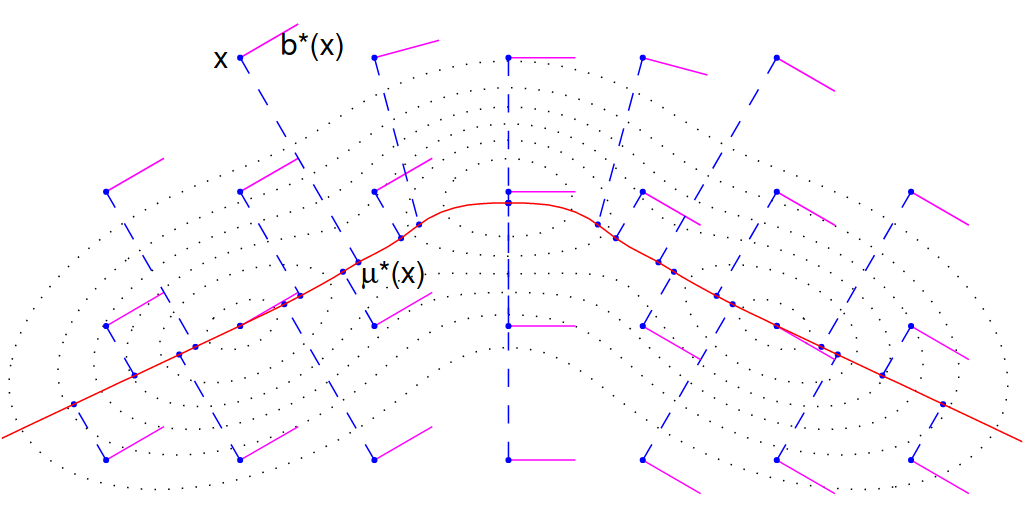
\includegraphics{deli}
	\caption{Illustration of the principal direction of a point $\boldsymbol x$}
\end{figure}

\subsubsection{Multivariate normal case}
\begin{prop}{}{}
	Let $\boldsymbol X \sim N_p(\mu,\, \Sigma)$. Let $\lambda_1$ be the largest eigenvalue of $\Sigma$
	and let $\boldsymbol v_1$ be the corresponding unit norm eigenvector.

	The following properties hold:
	\begin{enumerate}
		\item For all $\boldsymbol x \in \mathds{R}^p$, the correspondence $\boldsymbol b^*$ is in
		      fact a function and: $\boldsymbol b^*(\boldsymbol x_0) = \boldsymbol v_1,\,\forall\boldsymbol x_0$.
		\item For all $\boldsymbol x \in \mathds{R}^p$, the point $\boldsymbol x_1 = \mu^*(\boldsymbol x_0)$
		      belongs to the straight line defined by the first principal component:
		      $\{\mu + s\boldsymbol v_1 \mid s \in \mathds R\}$
		\item A point $\boldsymbol x \in \mathds{R}^p$ belongs to the first principal component
		      straight line if and only if $\boldsymbol x_1$ is a fixed point of the function
		      $\boldsymbol \mu^*$, that is if and only if $\boldsymbol x_1 = \boldsymbol \mu^*(\boldsymbol x_1)$.
	\end{enumerate}
\end{prop}

Only \emph{local information} around the hyperplane $H(\boldsymbol x, \boldsymbol v)$ is required
to check whether or not the pair $(\boldsymbol x, \boldsymbol v)$ identifies the first principal
component.

A mechanism to find points in the first principal component iterating the function
$\mu^*$ we arrive (in just on step) from any point
$\boldsymbol x_0$ to a point $\boldsymbol x_1$ in the first principal component.

The idea of looking for points $\boldsymbol x$ that are fixed points of the application
$\boldsymbol \mu^*$ easily generalizes when the v.a. $\boldsymbol X$ does not have a normal
distribution.

\begin{definition}{Principal oriented points (POP)}{}\index{POP}\index{principal oriented points}
	The set of fixed points of $\boldsymbol \mu^*$:
	\begin{equation*}
		\Gamma(\boldsymbol X) = \left\{
		\boldsymbol x \in \mathds{R}^p \mid \boldsymbol x = \boldsymbol \mu^*(\boldsymbol x)
		\right\}
	\end{equation*}
\end{definition}

\begin{definition}{Principal curve of oriented points (PCOP)}{}

	Let $\alpha : \mathds{R} \to \mathds{R}^p$ be a continuous curve parameterized by the arc length.
	We say that $\alpha$ is a \iemph{principal curve of oriented points} for $\boldsymbol X$ if:
	\begin{equation*}
		\left\{
		\alpha(s) \mid s \in [a,\, b]
		\right\} \subseteq \Gamma(\boldsymbol X)
	\end{equation*}
	\tcblower
	The former Proposition states that the first principal component is a PCOP
	for a r.v. $\boldsymbol X \sim N_p(\mu, \Sigma)$. Moreover the remaining principal
	components are not PCOPs.
\end{definition}

\begin{definition}{Probability distribution by a PCOP over an interval}{}
	The probability distribution over the interval $[a, b]$ induced by $\boldsymbol X$ and $\alpha$
	is the distribution of a r.v. $S$ having density function:
	\begin{equation*}
		f_S(s) \propto f_1(\alpha(s),\, b^*(\alpha(s))),\,s\in[a,\, b]
	\end{equation*}
	\tcblower
	Where $f_1$ is the one-dimensional density function obtained by integrating
	the joint density of $\boldsymbol X$ over the hyperplane $H(\alpha(s),\, b^*(\alpha(s)))$
	assuming that $\int_a^b f_S(s) ds < \infty$.

	Without loss of generality, we can assume that $S$ has expectation 0.
\end{definition}

\begin{theorem}{Existence of POPs and PCOPs}{}
	Let $\boldsymbol X$ be a r.v. with density function $f \in C^r,\, r \geq 2$.
	Assume that $\mu^*$ is a function (i.e. $|\boldsymbol \mu^*(\boldsymbol x)| = 1,\,\forall
		\boldsymbol x \in \text{Support}(\boldsymbol X)$. Then, $\Gamma(\boldsymbol X)$ is a
        \emph{non-empty set}.
	\tcblower
	\begin{note}
        To assume that $\mu^*$ is a function is a \emph{non-restrictive assumption}.
	\end{note}
\end{theorem}

\begin{definition}{Non-restrictive assumption}{}
	A non-restrictive assumption is an assumption that is not restrictive enough to
	be considered as a hypothesis.
\end{definition}

\begin{theorem}{Existence of a PCOP in the neighbourhood of a POP}{}
	Let $\boldsymbol X$ be a r.v. with density function $f \in C^r,\, r \geq 2$.
	Assume that the correspondence $\boldsymbol b^*$ is a function.

	Let $\boldsymbol x_0$ be a POP in the interior of $\text{Support}(\boldsymbol X)$.
	Then, there exists a PCOP $\alpha$ in a neighbourhood of $\boldsymbol x_0$:

	There exists $\varepsilon > 0$ and a curve $\alpha : (-\varepsilon,\, \varepsilon) \to \mathds{R}^p$
	such that $\alpha(0) = \boldsymbol x_0$ and $\alpha(t)$ is a POP for all $t \in (-\varepsilon,\, \varepsilon)$.

	\tcblower

	\begin{question}{Does $\alpha'(t)$ coincide with $b^*(\alpha(t))$?}{}
		In general, \emph{no}.
	\end{question}

	\begin{note}
		\emph{Uniqueness of the PCOP}: There are r.v. having a unique PCOP and there
		are other r.v. having several PCOPs (and even infinitely many).
	\end{note}
\end{theorem}

% \subsection{Non-Statistical Principal Curves}

\pagebreak
\section{Local MDS}

PCA does not work for non-linear configurations. MDS depends on the distance that is
used, Euclidean distance does not work for non-linear configurations.

\begin{note}
	Local MDS differentiates between \emph{short} and \emph{large} distances between
	pairs of objects:
	\begin{description}
		\item[Short distances] are managed as in MDS.
		\item[Large distances] a new term is added to introduce \iemph{repulsion} between the
			corresponding points in the low-dimensional configuration.
	\end{description}
\end{note}

\subsection{Definition}

Define $\mathcal N_K$ to be the symmetric set of nearby pairs of points.

Specifically, a pair $(i, j)$ is in $\mathcal N_K$ if point $i$ is among the $K$-nearest
neighbours of point $j$ and vice versa.

Then construct the \iemph{local stress function}:
\begin{equation*}
	\text{STRESS}_L(\boldsymbol X,\, \boldsymbol Y) = \sum_{(i,\, j) \in \mathcal N_K} (\delta_{ij} - d_{ij})^2
	+ \sum_{(i,\, j) \notin \mathcal N_K} w(D_\infty - d_{ij})^2
\end{equation*}
where $D_\infty$ is some large constant and $w$ is a small weight.

$\boldsymbol D = (\delta_{ij})^n_{i,\,j=1}$, the $n \times q$ matrix $\boldsymbol X$, and
$d_{ij} = \lVert \boldsymbol x_i - \boldsymbol x_j \rVert$ are defined as in non-classical
metric scaling (\cref{sec:non-classical-metric-scaling}).

\begin{problem}{Local MDS}{}
\begin{equation*}
	\min_{\boldsymbol X \in \mathds{R}^{n \times q}} \text{STRESS}_L(\boldsymbol X,\, \boldsymbol Y)
\end{equation*}
\end{problem}

\begin{question}{Could Local MDS be even more local?}{} No

	One could consider convenient to only consider the short distances and ignore
	the large ones. This is equivalent to using $w = 0$ in Local MDS. This has been
	tried several times but it does not work:
    \tcblower
	\begin{quote}
		Removing large distances from the stress function has been tried
		many times, but the hope that small dissimilarities add up to globally
		meaningful optimal configurations have always been frustrated.

		In some examples, removal of the largest third had \emph{calamitous
        effects} by reducing optimal configurations to mere disorder.
	\end{quote}
\end{question}

\subsection{Local continuity Meta-criteria}

The local continuity meta-criteria is a criteria for tuning parameter
selection in Local MDS that is also useful for other
dimensionality reduction methods.

For a neighbourhood size $K'$ and for the $i$-th object $\mathcal O_i$ in the
data set, let $N_{K'}(i)$ be the number of cases that simultaneously are between
the $K'$-nearest neighbours of $\mathcal O_i$ in the high-dimensional space
(distances here are $\delta_{ij}$) and between the $K'$-nearest neighbours of
the mapped point $\boldsymbol x_i$ in the low-dimensional space (distances here
are $\lVert \boldsymbol x_i - \boldsymbol x_j \rVert$).

We define
\begin{equation*}
	N_{K'} = \frac{1}{n} \sum_{i=1}^n N_{K'}(i)
\end{equation*}
as a global measure of overlapping between the $K'$-nearest neighbours in
both spaces, that could be called \iemph{local continuity}.

In order to normalize,
\begin{equation*}
	M_{K'} = \frac{N_{K'}}{K'}
\end{equation*}
is used instead of $N_{K'}$ ($M_{K'} \in [0, 1]$).

Even better, we can use the \iemph{adjusted local continuity meta-criteria}:
\begin{equation*}
	M_{K'}^{\text{adj}} = M_{K'} - \frac{K'}{n - 1}
\end{equation*}
because $K'/(n-1)$ is the expected value of $M_{K'}$ under complete
absence of association between the original data and the low-dimensional
configuration.

\subsection{Software}

As this moment (November 2022) there is no R implementation of Local MDS
in the CRAN repository.

There is the function \texttt{lmds} from package \texttt{stops} in R-forge.


\clearpage
\section{Isometric Feature Maping (ISOMAP)}

ISOmetric feature MAPping (ISOMAP) is a non-linear dimensionality reduction
method that is based on the idea of \emph{geodesic distances}.

\begin{algorithm}{ISOMAP}{ISOMAP}
	\begin{algorithmic}[1]
		\Procedure{ISOMAP}{$D_{\mathcal X}$} \Comment{$D_{\mathcal X}$ is the matrix of observed Euclidean distances}
		\State Identify neighbourhood relations ($\varepsilon$ or $k$) and define the
		corresponding graph $G^\varepsilon$.
		\State Compute shortest paths in $G^\varepsilon: D_{G,\varepsilon}$.
		\State Do MDS on $D_{G,\varepsilon}$.
		\State \Return Configuration in a low-dimensional space $\mathcal{\tilde{Y}}$.
		\EndProcedure
	\end{algorithmic}
\end{algorithm}

\begin{figure}[H]
	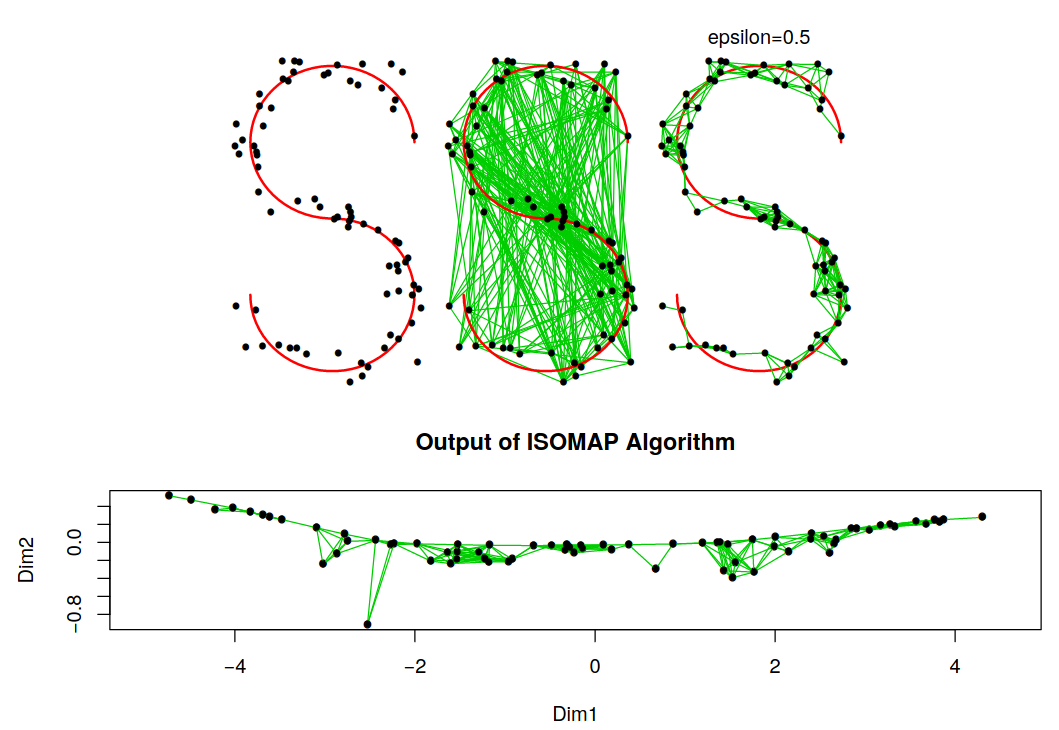
\includegraphics{isomap}
	\caption{Output of the ISOMAP algorithm.}
\end{figure}

\subsection{Role of the bandwidth parameter}
ISOMAP only depends on a tuning parameter $\varepsilon$ or $k$ that is used to
define the neighbourhood relations.

\begin{marker}
    The result if \emph{very} sensible to the \emph{bandwidth} value and can result
	in short-circuits or fragmented graph $G^\varepsilon$.
\end{marker}

There are several methods to select the bandwidth parameter, but there
is no consensus on which one is the best.

\pagebreak
\section[t-Stochastic Neighbor Embedding]{t-Stochastic Neighbor Embedding (t-SNE)}
\sectionmark{t-SNE}

\subsection{Stochastic Neighbor Embedding (SNE)}
It is an alternative to Local MDS or ISOMAP.

SNE requires a distance matrix $\boldsymbol D$ of size $n \times n$ with
entries $\delta_{ij} \geq 0$, the dissimilarity (or distance) between
individuals $i$ and $j$.

Alternatively, starting from a data matrix $\boldsymbol X$ of size $n \times p$,
(with $p$ variables and $n$ individuals), one can compute the pairwise
Euclidean distances $\boldsymbol D$: $\delta_{ij} = \lVert \boldsymbol x_i - \boldsymbol x_j \rVert$.

SNE starts by converting the high-dimensional distances between data points
into conditional probabilities $p_{i \mid j}$ that represent similarities:
\begin{equation*}
	p_{i \mid j} =
	\begin{cases}
		\frac{\exp(-\delta_{ij}^2 / 2\sigma_i^2)}{\sum_{k \neq i} \exp(-\delta_{ik}^2 / 2\sigma_i^2)} & \text{if } i \neq j \\
		0                                                                                             & \text{if } i = j
	\end{cases}
\end{equation*}
where $\sigma_i$ is a data-point dependent \iemph{bandwidth} parameter.

\begin{note}
	$p_{i \mid j}$ is the probability that a point $\boldsymbol x_i$ would pick
	point $\boldsymbol x_j$ as its neighbour if neighbours were picked in proportion
	to their probability density under a Gaussian centered at $\boldsymbol x_i$.
\end{note}

For the low-dimensional counterparts $\boldsymbol y_i$ and $\boldsymbol y_j$ of
the high-dimensional points $\boldsymbol x_i$ and $\boldsymbol x_j$, a similar
conditional probability is computed:
\begin{equation*}
	q_{i \mid j} =
	\begin{cases}
		\frac{\exp(-\lVert \boldsymbol y_i - \boldsymbol y_j \rVert^2)}{\sum_{k \neq i} \exp(-\lVert \boldsymbol y_k - \boldsymbol y_i \rVert^2)} & \text{if } i \neq j \\
		0                                                                                                                                         & \text{if } i = j
	\end{cases}
\end{equation*}
In this case, the same bandwidth $\frac{1}{\sqrt{2}}$ is used for every $\boldsymbol y_i$.

This way, every point $\boldsymbol y_i$ in the low-dimensional configuration will be
equally densely surrounded by its neighbours, leading to a better visualization.

If the low-dimensional points $\boldsymbol y_i$ and $\boldsymbol y_j$ correctly model
the similarity between the high-dimensional data points $\boldsymbol x_i$ and $\boldsymbol x_j$,
then the conditional probabilities $p_{i \mid j}$ and $q_{i \mid j}$ will be equal.

\begin{marker}
	SNE aims to find a low-dimensional data representation that minimizes
	the mismatch between the conditional probabilities $p_{i \mid j}$ and $q_{i \mid j}$.
\end{marker}

\begin{definition}{Kullback-Leibler divergence}
	The Kullback-Leibler divergence between two probability distributions $p$ and $q$ is defined as:
	\begin{equation*}
		KL(p \mid\mid q) = \sum_{j} p_j \log \frac{p_j}{q_j}
	\end{equation*}
	\tcblower
	\begin{note}
        Kullback-Leibler divergence is \emph{not symmetric}: there is a large
		cost for using widely separated map points $\boldsymbol y_i$ to
		represent nearby data points $\boldsymbol x_j$, but there is only a small
		cost for using nearby map points to represent widely separated data points.
	\end{note}
\end{definition}

\begin{problem}{Stochastic Neighbor Embedding (SNE)}{}

SNE minimizes (in a gradient descent fashion) the sum of Kullback-Leibler
divergences between the conditional distributions over all data points:
\begin{equation*}
	C(\boldsymbol Y) = \sum_{i=1}^n KL(P_i \mid\mid Q_i) =
	\mathlarger{\sum_{i=1}^n} \sum_{j=1}^n p_{i \mid j} \log \frac{p_{i \mid j}}{q_{i \mid j}}
\end{equation*}
\tcblower
\begin{note}
    The SNE cost function focuses on retaining the \emph{local structure} of the data in
	the map.
\end{note}
\end{problem}

\subsubsection{Choosing $\sigma_i$}

\begin{definition}{Shannon entropy}{}
	The Shannon entropy of a probability distribution $P$ is defined as:
	\begin{equation*}
		H(P) = - \sum_{j} p_j \log_2 p_j
	\end{equation*}
\end{definition}

\begin{definition}{Perplexity}{}
	The perplexity of a probability distribution $P$ is defined as:
	\begin{equation*}
		\text{Perp}(P) = 2^{H(P)}
	\end{equation*}
	\tcblower
	We can interpret it as the number of possible points in a uniform
	distribution having the same Shannon entropy as $P$.
	\tcbline
	\begin{note}
		When applied to the conditional distribution $P_i = \{p_{j\mid i}\}^n_{j=1}$,
		the perplexity is a measure of the number of neighbours that each point has.
	\end{note}

\end{definition}

\begin{marker}
	SNE performs a binary search to find the $\sigma_i$ that produces a
	$P_i$ with the desired perplexity (specified by the user).
\end{marker}

This method is fairly robust and typical values for the desired perplexity
range from 5 to 50.

\subsubsection{Symmetric cost function}
In order to improve the gradient descent, we can use a modified cost function
that is symmetric:
\begin{align*}
	q_{ij}           & = \frac{\exp(-\lVert \boldsymbol y_i - \boldsymbol y_j \rVert^2)}{\sum_{k \neq i} \exp(-\lVert \boldsymbol y_k - \boldsymbol y_i \rVert^2)} \\
	p_{ij}           & = \frac{p_{i \mid j} + p_{j \mid i}}{2n}                                                                                                    \\
	C(\boldsymbol Y) & =
	\mathlarger{\sum_{i=1}^n} \sum_{j=1}^n p_{ij} \log \frac{p_{ij}}{q_{ij}}
\end{align*}

\subsubsection{The crowding problem of SNE}
If the intrinsic dimension of the observed object is moderate (say 10),
the standard 2-dimensional dimensionality reduction, performed for
visualization, can not give good results. Since pairwise distances
in a 2-dimensional space cannot faithfully model distances between points
on the 10-dimensional manifold, the resulting map will be very \iemph{crowded}.

\begin{marker}
	In practice, the consequence of the crowding problem is that many
	high-dimensional points that are at moderate distance from the
	center of the data, are crushed together in the center of the
	low-dimensional map, which prevents gaps from forming between the
	natural clusters.
\end{marker}

The crowding problem is not specific to SNE, it also affects other
dimensionality reduction techniques such as non-classical metric MDS,
Local MDS or ISOMAP.

To solve this problem, we need to use t-SNE instead.

\subsection{t-Stochastic Neighbor Embedding (t-SNE)}

The main change in t-SNE with respect to SNE is the way the joint
probabilities $q_{i \mid j}$ for $i \neq j$ are computed:
\begin{equation*}
	q_{i \mid j} = \frac
	{
		(1 + \lVert \boldsymbol y_i - \boldsymbol y_j \rVert^2)^{-1}
	}{
		\sum_{k \neq i} (1 + \lVert \boldsymbol y_k - \boldsymbol y_i \rVert^2)^{-1}
	}
\end{equation*}
That is, a Student's t-distribution with 1 degree of freedom (A Cauchy distribution)
is used to transform the distances in the low dimensionality.

Additionally, t-SNE uses the symmetric version of the cost function.

\subsubsection{Software}
\begin{itemize}
	\item \texttt{tsne} fully implemented in R.
	\item \texttt{Rtsne} R interface to the a C++ implementation of t-SNE.
\end{itemize}

% \section{t-Stochastic Neighbor Embedding}


% Non-parametric regression models
%! TEX root = ../000-main.tex
\part{Non-parametric regression models}

%! TEX root = ../000-main.tex
\chapter{Non-parametric regression model}
\chaptermark{NP reg. model}

\section{Introduction}

\begin{definition}{Regression function}{}

	Let $(X,\, Y)$ be random variables with continuous joint distribution.

	The best prediction (in the sense of the minimum mean squared prediction error)
	of the dependent variable $Y$ given that the independent variable $X$ takes
	the known value $x$ is the conditional expectation of $Y$ given $X=x$:
	\begin{equation*}
		m(x) = \mathds{E}( Y \mid X = x)
	\end{equation*}
	also known as \iemph{regression function}.
\end{definition}

\subsection{Parametric regression model}

The \iemph{parametric regression model} assumes that the regression function
is known except for a fixed finite number of parameters.

\begin{example}{Simple linear regression model}{}
	\begin{equation*}
		y = \beta_0 + \beta_1 X + \varepsilon
	\end{equation*}
	So the regression function is $m(x) = \beta_0 + \beta_1 x$ is known except
	for the parameters $\beta_0$ and $\beta_1$.
\end{example}

\subsection{Non-parametric regression model}

In the \iemph{non-parametric regression model} the functional form of the
regression function $m(x)$ is not specified.

\begin{note}
	However, certain regularity conditions are assumed. For instance,
	it is usually assumed that $m(x)$ has a continuous second derivative.
\end{note}

\begin{question}{What does it mean to fit a non-parametric regression model?}{}
	To provide an estimator $\hat{m}(t)$ of the regression function $m(t)$ for
	all $t \in \mathbb{R}$.

	This usually implies to draw the graphic of the pairs $(t,\, \hat{m}(t))$ where
	$t_j,\, j=1,\ldots,J$ is a regular fine grid covering the range of observed values
	$x_i,\, i=1,\ldots,n$.
	Alternatively, an algorithm that computes the values $\hat{m}(t)$ for any $t$
	can be provided.

	We also have give an estimator $\hat\sigma^2$ of the residual variance $\sigma^2$.
\end{question}

\clearpage
\section{Local polynomial regression}
\subsection{Local linear regression}

\paragraph{Initial idea} Divide the range of $X$ into $K$ disjoint intervals
each of them showing an \iemph{approximately linear} relationship between $X$ and $Y$.
\begin{figure}[H]
	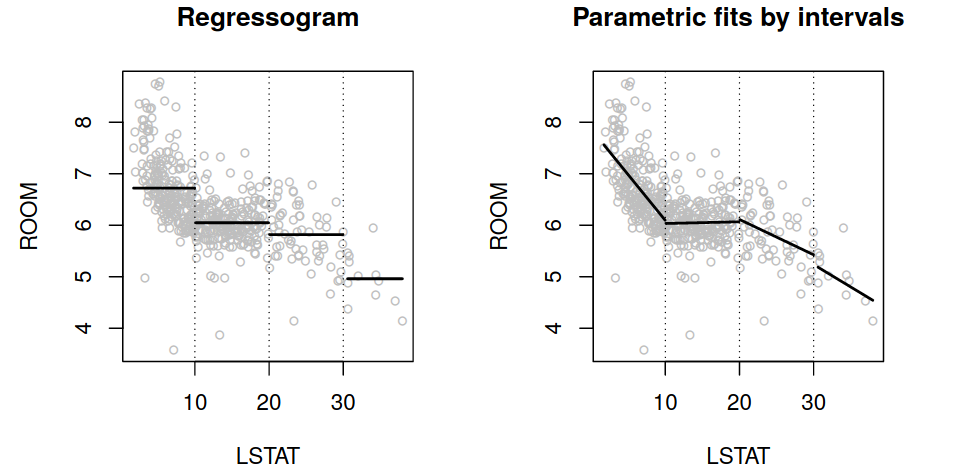
\includegraphics{ll_init}
	\caption{Initial idea of local linear regression.}
\end{figure}

This provides good results, but its not satisfactory, we apply to improvements:
\begin{description}
	\item[Localizing] In order to estimate the regression function at a given value $t$,
		use the data $(x_i,\, y_i)$ such that $x_i$ is in an interval centered at $t$.
	\item[Smoothing] Assign to each datum $(x_i,\, y_i)$ a weight $w_i$ that decreases
		as $|x_i - t|$ increases.
\end{description}

\begin{definition}{datum}{}
	A datum is a pair $(x_i,\, y_i)$ where $x_i$ is the value of the independent
	variable and $y_i$ is the value of the dependent variable.
\end{definition}

\subsubsection{Local linear fitting}
Weights are assigned by a \iemph{kernel function} $K$: usually a
symmetric unimodal density function centered at $0$.

The weight of $(x_i, y_i)$ is when estimating $m(t)$ is:
\begin{equation*}
	w_i = w(t,\,x_i) = K \left. \left( \frac{x_i - t}{h} \right) \middle/ \sum_{j=1}^n K \left( \frac{x_i - t}{h} \right) \right.
\end{equation*}
where $h$ is the \iemph{smoothing parameter} or \iemph{bandwidth}.

\begin{note}
	The final estimate is significantly affected by the choice of the bandwidth, so this
	choice is crucial in non-parametric estimation.
\end{note}

\begin{figure}[H]
	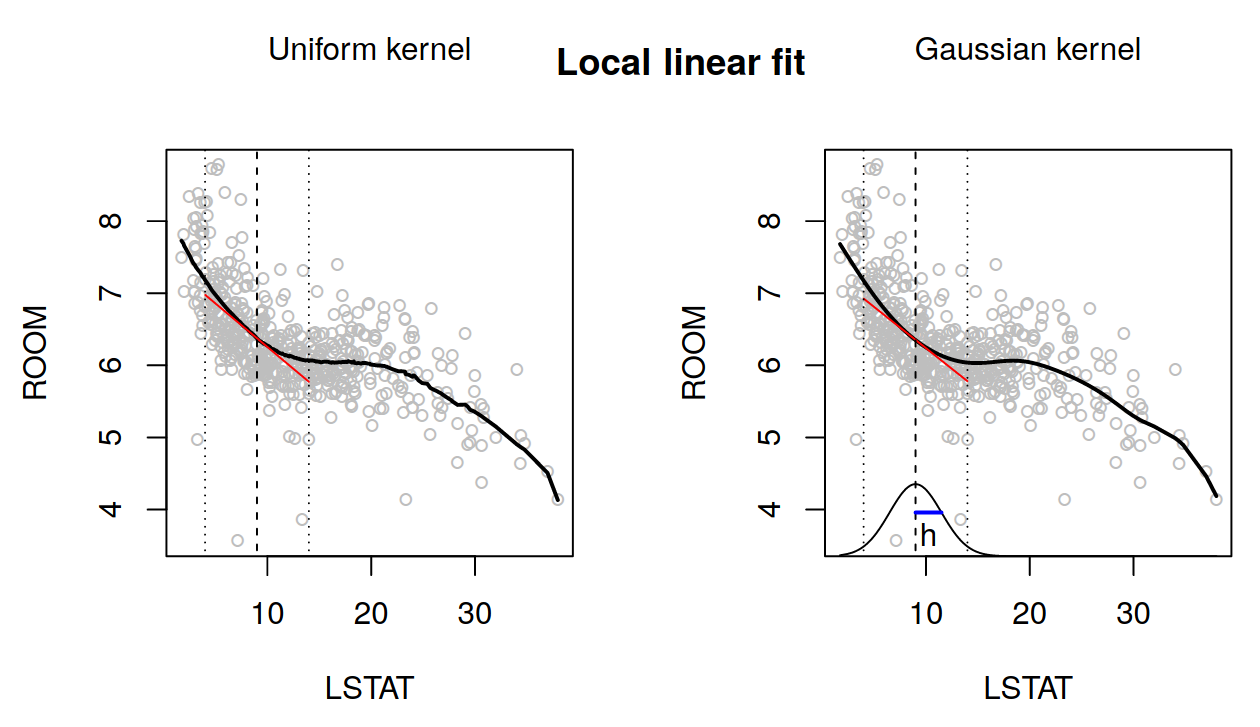
\includegraphics{ll_fit}
	\caption{Local linear fit with different kernel choices.}
\end{figure}

\subsection{Local polynomial regression}
Consider the weighted polynomial regression problem:
\begin{problem}{Weighted polynomial regression problem}{}
\begin{equation*}
	\min_{\beta_0,\ldots,\beta_q} \mathlarger{\sum_{i=1}^n} w_i \left( y_i - \beta_0 - \sum_{j=1}^q \beta_j x_i^j \right)^2
\end{equation*}
\end{problem}
Observe that the estimated coefficients depend on $t$, the
point for which the regression function is being estimated: $\hat\beta_j = \hat\beta_j(t)$.

The proposed estimate for $m(t)$ is the value of the locally fitted
polynomial $P_{q,t}(x) = \sum_{j=0}^q \hat\beta_j(x - t)^j$ at $x = t$:
\begin{equation*}
	\hat{m}(t) = P_{q,t}(t) = \hat\beta_0(t)
\end{equation*}

Moreover, the estimated polynomial $P_{q,t}(x)$ allows us to estimate the first $q$ derivatives
of $m$ at $t$:
\begin{equation*}
	\hat{m}_q^{(r)}(t) = \frac{d^r}{dx^r} P_{q,t}(t) {\Bigm|_{x=t}} = r! \hat\beta_r(t)
\end{equation*}

\subsubsection{Particular case: Nadaraya-Watson estimator}
\begin{definition}{Nadaraya-Watson estimator}{}
	When the degree of the locally fitted polynomial is \emph{$q=0$} (i.e. a constant),
	the resulting non-parametric estimator is called \iemph{Nadaraya-Watson estimator}
	or \iemph{kernel estimator}:
	\begin{equation*}
		\hat m_K(t) = \frac{
			\sum_{i=1}^n K \left( \frac{x_i - t}{h} \right) y_i
		}{
			\sum_{i=1}^n K \left( \frac{x_i - t}{h} \right)
		} = \sum_{i=1}^n w(t, x_i) y_i
	\end{equation*}
	\tcblower

	This was proposed before local polynomial estimators.

	\begin{note}
		\paragraph{Observe:} $\hat m_K(t)$ is a \iemph{moving weighted average}.
	\end{note}

\end{definition}


\begin{prop}{Every local polynomial estimator is itself a weighted average}{}
	\begin{equation*}
		\hat m_{q}(t) = \sum_{i=1}^n w_q^*(t,\, x_i) y_i
	\end{equation*}
	But the weights $w_q^*(t,\, x_i)$ are not necessarily non-negative.
\end{prop}

\subsubsection{Matrix formulation of the local polynomial estimator}
Let
\begin{equation*}
	X_t = \begin{pmatrix}
		1      & x_1 - t & \ldots & (x_1 - t)^q \\
		1      & x_2 - t & \ldots & (x_2 - t)^q \\
		\vdots & \vdots  & \ddots & \vdots      \\
		1      & x_n - t & \ldots & (x_n - t)^q
	\end{pmatrix}
\end{equation*}
be the \iemph{regressor matrix}.

We define $Y = (y_1, \ldots, y_n)^T,\, \varepsilon = (\varepsilon_1, \ldots, \varepsilon_n)^T,\,
	\beta = (\beta_0, \ldots, \beta_q)^T$ and we let $W_t = \text{diag}(w(x_1, t), \ldots, w(x_n,t))$
be the \iemph{weight matrix}.

We fit the regression model $Y = X_t\beta + \varepsilon$ using weighted least squares:
\begin{align*}
	\hat\beta & = \argmin_{\beta\in\mathbb{R}^{q+1}} \sum_{i=1}^n w_i(y_i - \beta_0 - \sum_{j=1}^q \beta_j x_i^j)^2 \\
	          & = \argmin_{\beta\in\mathbb{R}^{q+1}} (Y - X_t\beta)^T W_t (Y - X_t\beta)
\end{align*}
The solution is:
\begin{equation*}
	\hat\beta = (X_t^T W_t X_t)^{-1} X_t^T W_t Y
\end{equation*}

For $j=0,\ldots,q$, let $e_j$ be the $(q+1)$-dimensional vector
having all its coordinates 0 except for the $(j+1)$-th one, which is 1.
Then:
\begin{equation*}
	\hat m_q(t) = \hat \beta_0 = e_0^T (X_t^T W_t X_t)^{-1} X_t^T W_t Y = S_tY = \sum_{i=1}^n w^*_q(t,\, x_i) y_i
\end{equation*}
where $S_t = e_0^T (X_t^T W_t X_t)^{-1} X_t^T W_t$ is an $n$-dimensional row vector (it
is in fact a \iemph{smoothing matrix}).

\begin{note}
	We say that the local polynomial regression estimator is a \iemph{linear smoother}
	because for a fixed $t$, $\hat m_q(t)$ is a linear function of $y_1,\ldots,y_n$.
\end{note}

The local polynomial estimator of the $r$-th derivative of $m$ at point $t$ is:
\begin{equation*}
	\hat m_q^{(r)}(t) = r!e_r^T\hat\beta_r(t) = r!e_r^T\hat\beta
\end{equation*}
which is also linear in $y_1,\ldots,y_n$.

\subsection{Linear smoothers}

\begin{definition}{Linear smoother}{}
	A non-parametric linear regression estimator $\hat m$ is said to be
	a \iemph{linear smoother} when for any fixed $t$, $\hat m(t)$ is a linear function of
	$y_1,\ldots,y_n$:
	\begin{equation*}
		\hat m(t) = \sum_{i=1}^n w(t, x_i) y_i
	\end{equation*}
	for some weight function $w$.
	\tcblower
	\begin{note}
		Linear smoothers are particular cases of linear estimators of the regression
		function, as \iemph{OLS} or \iemph{ridge regression}.
	\end{note}
\end{definition}

\begin{definition}{Smoothing matrix}{}

	Let
	\begin{equation*}
		\hat y_i = \hat m (x_i) = \sum_{j=1}^n w(x_i, x_j) y_j
	\end{equation*}
	be the fitted values for the $n$ observed values  $x_i$ of the explanatory variable.

	In matrix format:
	\begin{equation*}
		\hat Y = S Y
	\end{equation*}
	where column vectors $Y$ and $\hat Y$ have elements $y_i$ and $\hat y_i$ respectively,
	and the matrix $S$ has generic element $s_{ij} = w(x_i, x_j)$.

	\begin{note}
		The matrix $S$ is called the \iemph{smoothing matrix}, because its effect on the observed
		data $(x_i, y_i)$ is to transform them into $(x_i, \hat y_i)$ which is a much
		smoother data configuration.
	\end{note}

	\tcblower
	The smoothing matrix is analogous to the \iemph{hat matrix} $H = X(X^TX)^{-1}X^T$ in
	multiple linear regression:
	\begin{equation*}
		\hat Y = X(X^TX)^{-1}X^T Y = H Y
	\end{equation*}
\end{definition}

\begin{prop}{Parameters in a linear smoother model}{effective-parameters}
	For a linear smoother with smoothing matrix $S$, the \iemph{effective
		number of parameters} is the sum of diagonal elements of $S$:
	\begin{equation*}
		\nu = \text{Trace}(S) = \sum_{i=1}^n s_{ii}
	\end{equation*}
	\tcblower
	\begin{note}
		The interpretation of $\nu$ as the effective number of parameters is
		valid for any linear non-parametric estimator.
	\end{note}

	We can thus compare the degree of smoothing of two linear non-parametric
	estimators just by comparing their effective number of parameters.
\end{prop}

\subsubsection{An estimator of $\sigma^2$}
An estimator of $\sigma^2$ in non-parametric estimation is:
\begin{equation*}
	\hat\sigma^2 = \frac{1}{n-\nu} \sum_{i=1}^n (y_i - \hat m(x_i))^2
\end{equation*}

\subsection{Kernel functions}

\begin{definition}{Kernel functions}{kernel-functions}
	Density functions with zero mean.
	\tcblower
	We can also rescale them so that they have zero mean and
	variance 1. Then we call them \iemph{rescaled kernels}.
\end{definition}

\begin{figure}[H]
	% 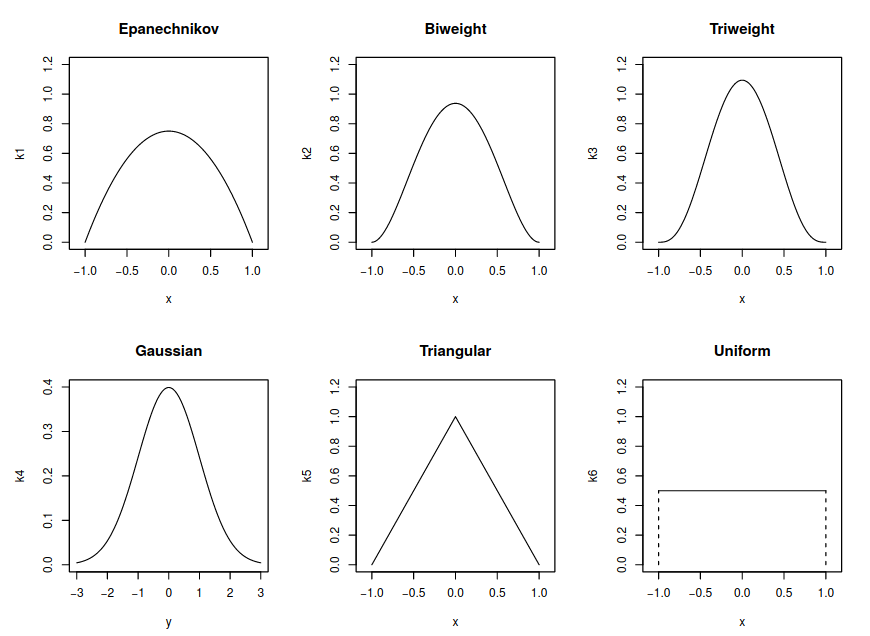
\includegraphics{kernel_examples}
	\begin{tikzpicture}
		\begin{groupplot}[group style={
						group size=3 by 2,
						xlabels at=edge bottom,
						ylabels at=edge left,
                        vertical sep=4em,
					},
				width = .3\textwidth,
				ymin=-0.1, ymax=1.1,
				xlabel=$x$, ylabel=$K(x)$,
                every axis plot/.append style={smooth, mark=none, line width=2pt},
                samples=25,
                domain=-1:1,
                xmin=-1.2, xmax=1.2
			]
            \nextgroupplot[title={\bfseries Epanechnikov ($K^*$)}]
			\addplot[ color=blue] {3/4*(1-x^2)*((x>=-1)*(x<=1))};

			\nextgroupplot[title={\bfseries Biweight}]
			\addplot[ color=red] {15/16*(1-x^2)^2*((x>=-1)*(x<=1))};

			\nextgroupplot[title={\bfseries Triweight}]
			\addplot[ color=green!70!black] {35/32*(1-x^2)^3*((x>=-1)*(x<=1))};

			\nextgroupplot[title={\bfseries Gaussian},xmin=-3.7, xmax=3.7]
			\addplot[domain=-3:3, color=orange] {1/sqrt(2*pi)*exp(-x^2/2)*2};

			\nextgroupplot[title={\bfseries Triangular}]
            \draw[line width=2pt, color=black] (-1,0) -- (0,1) -- (1,0);

			\nextgroupplot[title={\bfseries Uniform}]
            \draw[line width=2pt, color=gray] (-1,0.5) -- (1,0.5);
            \draw[line width=2pt, color=gray,dashed] (-1,0) -- (-1,0.5);
            \draw[line width=2pt, color=gray,dashed] (1,0) -- (1,0.5);
		\end{groupplot}
	\end{tikzpicture}
	\caption{Examples of Kernel functions used in non-parametric estimation}
\end{figure}

\begin{table}[H]
	\caption{Examples of Kernel functions used in non-parametric estimation}
	\begin{tabular}{lccl}
		\toprule
		Kernel ($K$)         & Expression                                & Variance & Efficiency \\
		\midrule
		Epanechnikov ($K^*$) & $\frac{3}{4}(1-x^2)I_{[-1,1]}(x)$         & $1/5$    & 1          \\
		Biweight             & $\frac{15}{16}(1-x^2)^2I_{[-1,1]}(x)$     & $1/7$    & 0.994      \\
		Triweight            & $\frac{35}{32}(1-x^2)^3I_{[-1,1]}(x)$     & $1/9$    & 0.987      \\
		Gaussian             & $\frac{1}{\sqrt{2\pi}}e^{-\frac{x^2}{2}}$ & $1$      & 0.951      \\
		Triangular           & $\frac{1}{2}(1-|x|)I_{[-1,1]}(x)$         & $1/6$    & 0.986      \\
		Uniform              & $\frac{1}{2}I_{[-1,1]}(x)$                & $1/3$    & 0.930      \\
		\bottomrule
	\end{tabular}
\end{table}

\subsection{Theoretical properties of local polynomial regression}

\subsubsection{Local Properties}

The \iemph{local behaviour} refers to the statistical properties of
a non-parametric estimate $\hat m(t)$ as estimator of the unknown
value $m(t)$ at a given point $t$.

\begin{definition}{Bias}{Bias}
	Let $m(t)$ be the true value of the regression function at $t$.
	The \iemph{bias} of a non-parametric estimator $\hat m(t)$ is:
	\begin{equation*}
		\text{Bias}_{m(t)}(\hat m(t)) = \mathbb E[\hat m(t)] - m(t)
	\end{equation*}
\end{definition}

\begin{definition}{Variance}{Variance}
	The \iemph{variance} of a non-parametric estimator $\hat m(t)$ is:
	\begin{equation*}
		\text{Var}_{m(t)}(\hat m(t)) = \mathbb E\bigl[(\hat m(t) - \mathbb E[\hat m(t)])^2\bigr]
	\end{equation*}
\end{definition}

\begin{definition}{Mean Squared Error (MSE)}{MSE}
	The \iemph{mean squared error} of a non-parametric estimator $\hat m(t)$ is:
	\begin{equation*}
		\text{MSE}_{m(t)}(\hat m(t)) = \mathbb E\bigl[(\hat m(t) - m(t))^2\bigr]
		= \text{Bias}_{m(t)}(\hat m(t))^2 + \text{Var}_{m(t)}(\hat m(t))
	\end{equation*}
\end{definition}

\begin{question}{Local properties}{}
	\begin{itemize}
		\item Is $\hat m (t)$ an unbiased estimator of $m(t)$? ($\text{Bias}_{m(t)}(\hat m(t)) = 0$)
		\item Is $\lim_{n\to\infty}\text{Var}_{m(t)}(\hat m(t)) = 0$?
		\item Is $\hat m (t)$ a consistent estimator of $m(t)$? Does $\hat m (t)$ converge to $m(t)$?
		\item Is $\lim_{n\to\infty}\text{MSE}_{m(t)}(\hat m(t)) = 0$?
	\end{itemize}
\end{question}

\subsubsection{Global Properties}

We talk about \iemph{global properties} when our interest is on $\hat m(t)$
as an estimator of $m(t)$ for all $t \in [a, b]$, where $[a, b]$ is the
interval where the explanatory variable $x$ takes its values.

\begin{question}{Global properties}{}
	Does the estimated function $\hat m$ converge to the unknown function $m$
	in some sense appropriate for functions?
	\tcblower
	One common way for measuring the distance between $\hat m$ and $m$ is
	the \emph{Integrated Mean Squared Error} (IMSE):
	\begin{equation*}
		\lim_{n\to\infty} \text{IMSE}_{m}(\hat m) = 0?
	\end{equation*}
\end{question}

\begin{definition}{Integrated Mean Squared Error (IMSE)}{IMSE}
	\begin{align*}
		\text{IMSE}_{m}(\hat m) & = \int_a^b \text{MSE}_{m(t)}(\hat m(t)) \, dt
		= \int_a^b \mathds{E}\bigl[(\hat m(t) - m(t))^2\bigr] \, dt                  \\
		                        & = \int_a^b \text{Bias}_{m(t)}(\hat m(t))^2 \, dt +
		\int_a^b \text{Var}_{m(t)}(\hat m(t)) \, dt
	\end{align*}
\end{definition}

\begin{theorem}{Bias and Variance of $\hat m_0(t)$ and $\hat m_1(t)$}{}
	Consider the non-parametric regression model:
	\begin{equation*}
		Y_i = m(X_i) + \varepsilon_i, \quad i = 1, \ldots, n
	\end{equation*}
	where $\varepsilon_1, \ldots, \varepsilon_n$ are independent r.v. with
	$\text{Var}(\varepsilon_i) = \sigma^2(x_i)$; $X_1, \ldots, X_n$ are
	independent r.v. with density $f$ and $P(a \leq X_i \leq b) = 1$ for some
	$a, b \in \mathbb R$. Assume the following regularity conditions:
	\begin{enumerate}
		\item $f(t) > 0\quad\forall t$.
		\item $f(t),\, m''(t)$ and $\sigma^2(t)$ are continuous in the neighborhood of $t$.
		\item $K$ is symmetric with support on $[-1, 1]$, $\int_R K(u) \, du = 1$ and
		      $\int_{-1}^1 K(u) \, du = 0$.
		\item $t \in (a, b)$.
		\item $h \to 0$ and $n\cdot h \to \infty$ when $n \to \infty$.
	\end{enumerate}
	\tcbline
	In this context, the following statements hold:
	\begin{enumerate}
		\item The \iemph{Nadaraya-Watson estimator} and the \iemph{local linear estimator}
		      both have the variance:
		      \begin{equation*}
			      \frac{\sigma^2(t)}{nhf(t)} \int_{-1}^1 K^2(u) \, du + o\left(\frac{1}{nh}\right)
		      \end{equation*}
		\item The \emph{Nadaraya-Watson estimator} has bias:
		      \begin{equation*}
			      \left(
			      \frac{m'(t)f'(t)}{f(t)} + \frac{m''(t)}{2}
			      \right)h^2
			      \int_{-1}^1 u^2K(u) \, du + o\left(h^2\right)
		      \end{equation*}
		\item The \emph{local linear estimator} has bias:
		      \begin{equation*}
			      \frac{m''(t)}{2} h^2
			      \int_{-1}^1 u^2K(u) \, du + o\left(h^2\right)
		      \end{equation*}
		\item The $\text{MSE}_{m(t)}(\hat m(t))$ is $O(h^4) + O(1/(nh))$ for both estimators.
		      Then, both converge to $m(t)$ in quadratic mean and in probability.
	\end{enumerate}
\end{theorem}

\subsubsection{Bias-Variance Tradeoff}
\begin{definition}{Asymptotic Mean Squared Error (AMSE)}{AMSE}\index{AMSE}\index{asymptotic mean squared error}
	Is the main part of the MSE (ignoring the infinitesimal terms).
\end{definition}

Let us consider the AMSE for the local linear estimator:
\begin{equation*}
	\text{AMSE}(h) = \underbrace{\frac{(m''(t))^2}{4}h^4 \left( \int_{-1}^1 u^2 K(u)\, du \right)^2}_{\text{bias}^2}
	+
	\underbrace{\frac{\sigma^2(t)}{nhf(t)} \int_{-1}^1 K^2(u) \, du}_{\text{variance}}
\end{equation*}

The first term, the squared bias, increases with $h$.

The second term, the variance, decreases with $h$.

\begin{note}
	The optimal value $h_{\text{AMSE}}$ represents the compromise between bias and variance.
\end{note}

\begin{figure}[H]
	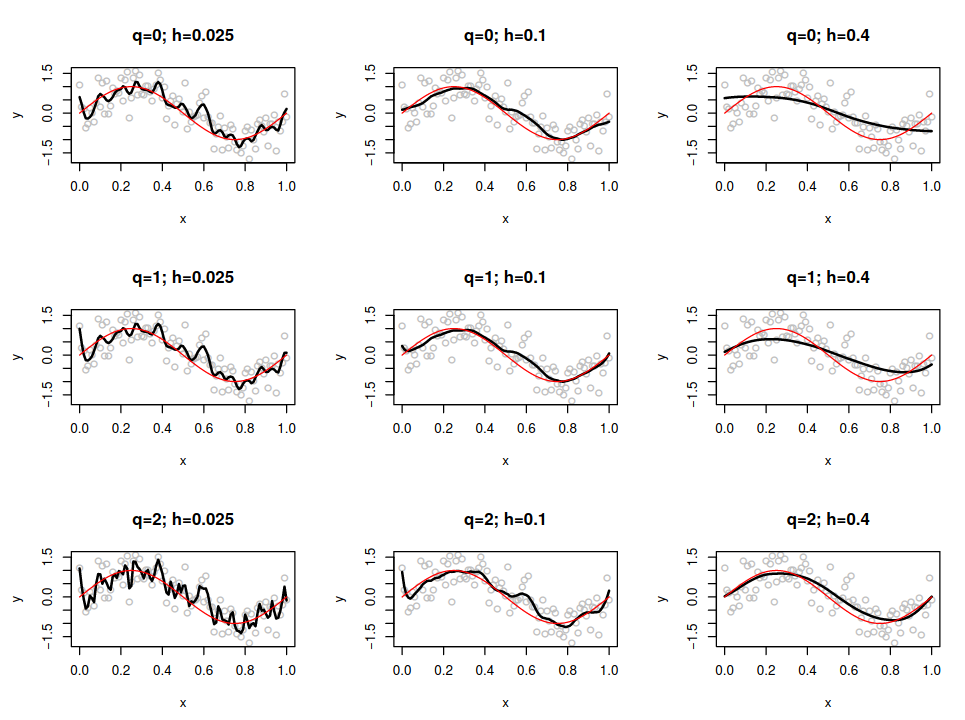
\includegraphics{effect_hq}
	\caption{Effect of bandwidth $h$ and degree $q$ on a single sample.}
\end{figure}

\subsection{Choosing the Smoothing Parameter (Bandwidth)}
The choice of the smoothing parameter $h$ is a crucial step in the appearance
and properties of the regression function estimator.

\begin{description}
	\item[Estimation]
		The bandwidth controls the \iemph{Bias-Variance Tradeoff}. With a small bandwidth,
		the estimator is highly variable and has small bias. With a large bandwidth, the
		opposite happens.
	\item[Prediction of New Observations] The smoothing parameter $h$ controls the
		balance between fitting the observed data well and the ability to predict
		new observations.

		Small values of $h$ give more flexibility, but the prediction errors
		will be higher (\iemph{overfitting}).

		If $h$ is too large, there is \iemph{underfitting}, as it may happen with
		global parametric models. In this case, both the errors in the observed data
		and the prediction will be high.
\end{description}

\paragraph{Criteria for Choosing the Smoothing Parameter}
There are several sensible criteria for choosing the smoothing parameter. We can
categorize them in two groups:
\begin{enumerate}
	\item \emph{Estimation quality} based methods (statistical perspective).
	\item \emph{Prediction error} based methods (machine learning perspective).
\end{enumerate}

\subsubsection{Estimation based criteria}

\paragraph{Integrated Mean Squared Error (IMSE)} We can minimize the
IMSE (\ref{def:IMSE}) to choose the bandwidth $h$ as shown in~\cref{fig:IMSE}.
\begin{figure}[H]
	\includegraphics{IMSE}
	\caption{IMSE for different values of $h$.}%
	\label{fig:IMSE}
\end{figure}

\begin{definition}{Mean Integrated Squared Error (MISE)}{MISE}\index{MISE}\index{mean integrated squared error}
	\begin{equation*}
		\text{MISE}(\hat m) = \mathds{E}_{\boldsymbol Z} \left[
			\int_a^b \left( m(t) - \hat m(t) \right)^2 f(t) \, dt
			\right] =
		\mathds{E}_{\boldsymbol Z} \left[
			\mathds{E}_T \left\{
			\left( m(T) - \hat m(T) \right)^2 \mid \boldsymbol Z
			\right\}
			\right]
	\end{equation*}
	where $\boldsymbol Z = \left\{(x_i,\, Y_i) \mid i = 1,\ldots,n\right\}$ is the sample
	used to estimate $\hat m$ and $T$ is a r.v. independent from $\boldsymbol Z$
	with the same distribution that generates the independent variable values $x_i$.
	\tcblower
	\begin{note}
		It coincides with IMSE by \iemph{Fubini's Theorem}.
	\end{note}
\end{definition}

\subsubsection{Prediction based criteria}
\begin{definition}{Predictive Mean Squared Error (PMSE)}{PMSE}\index{PMSE}\index{predictive mean squared error}
	Is the expected squared error made when predicting $Y = m(t) + \varepsilon$ by $\hat m(t)$.
	Where $t$ is an observation of the r.v. $T$, distributed as the observed explanatory variable.

	When $T$ and $\varepsilon$ are independent from the sample $\boldsymbol Z$, then:
	\begin{align*}
		\text{PMSE}(\hat m) & = \mathds{E}_{\boldsymbol Z,(T,Y)} \left[
			\left(Y - \hat m(T)\right)^2
			\right]
		= \mathds{E}_{\boldsymbol Z,T,\varepsilon} \left[
			\left(\hat m(T) - m(T) - \varepsilon\right)^2
		\right]                                                         \\
		                    & = \mathds{E}_{\boldsymbol Z,T} \left[
			\left(\hat m(T) - m(T)\right)^2
			\right] + \mathds{E}_\varepsilon\left[\varepsilon^2\right]
		= \text{MISE}(\hat m) + \sigma^2
	\end{align*}
	\tcblower
	\begin{note}
		MISE and PMSE are equivalent when $T$ and $\varepsilon$ are independent from $\boldsymbol Z$.
	\end{note}
\end{definition}

\begin{marker}
	Unfortunately, both IMSE, MISE and PMSE are \emph{unfeasible} to compute
	because they require the knowledge of the \emph{true} regression function
	$m$ (which is unknown in practice).
\end{marker}

\begin{definition}{Residual Sum of Squares (RSS)}{RSS}\index{RSS}\index{residual sum of squares}
	Is an \emph{optimistic} estimation of PMSE:
	\begin{equation*}
		\text{RSS}(\hat m) = \frac{1}{n} \sum_{i=1}^n \left( Y_i - \hat m(x_i) \right)^2
	\end{equation*}
	\tcblower
	\begin{note}
		Also known as the \iemph{error in the training sample}
	\end{note}
\end{definition}

Only the RSS is feasible to compute, but it is not a good estimator of PMSE
since it is \emph{optimistically} biased.

\subsubsection{Bandwidth Selection in Practice}
As we have seen, the proposed criteria are not feasible to compute. We have several
alternatives based in a train, test (and validation) split of the data.
\begin{itemize}
	\item Minimizing the average squared prediction error in a validation set.
	\item Leave-one-out cross-validation.
	\item K-fold cross-validation.
	\item Generalized cross-validation (Only for linear estimators)
\end{itemize}

\begin{definition}{Validation set}{}
	When the available data is large enough, we can randomly split it into
	3 sets:
	\begin{enumerate}
		\item \iemph{Training set}: Used to fit the model.
		\item \iemph{Validation set}: Used for model selection and parameter tuning.
		\item \iemph{Test set}: Used to evaluate the generalization of the final model.
	\end{enumerate}
\end{definition}

\begin{definition}{$\text{PMSE}_\text{Val}$}{PMSEVal}
	We can choose the bandwidth $h_\text{Val}$ by minimizing the
	Predictive Mean Squared Error in the validation set:
	\begin{equation*}
		\text{PMSE}_\text{Val}(h) = \frac{1}{n_V} \sum_{i=1}^{n_V} \left( Y_i^V - \hat m(x_i^V) \right)^2
	\end{equation*}
	where $(x_i^V,\, Y_i^V),\,i=1,\ldots,n_V$ are the observations of the validation set and
	$\hat m$ is the estimator with bandwidth $h$ using the training set.
\end{definition}

\begin{definition}{Leave-one-out cross-validation (LOOCV)}{LOOCV}
	\begin{enumerate}
		\item For each observation $(x_i,\, Y_i)$ of the training set, we fit the model
		      using the remaining observations.
		\item We compute the squared prediction error for the observation $(x_i,\, Y_i)$
		      using the fitted model.
		\item We average the squared prediction errors.
	\end{enumerate}
	\begin{equation*}
		\text{PMSE}_\text{LOOCV}(h) = \frac{1}{n} \sum_{i=1}^n \left( Y_i - \hat m_h(x_i) \right)^2
	\end{equation*}
	\tcblower
	\begin{note}
		LOOCV is a good alternative when the number of observations is small and we cannot
		afford to split the data into 3 sets.
	\end{note}
	\begin{note}
		LOOCV is a special case of K-fold cross-validation with $K=n$.
	\end{note}
	\begin{note}
		$\text{PMSE}_\text{LOOCV}(h)$ is an approximately unbiased estimator of $\text{PMSE}(h)$,
		but has a high variance.
	\end{note}
\end{definition}

\begin{definition}{$K$-fold cross-validation}{}
	Instead of taking one observation, we split the training set into $K$ subsets
	and remove whole subsets at each iteration.

	\tcblower
	\begin{note}
		$K$-fold cross-validation has lower variance than LOOCV, but larger bias.
	\end{note}
	Usually we use $K=5$ or $K=10$.
\end{definition}

\begin{definition}{Generalized cross-validation (GCV)}{GCV}
	For linear smoothers, a modification can be done in the measure
	of $\text{PMSE}_\text{CV}$.

	It consists in replacing the values of $s_{ii}$ coming
	from the diagonal of $S$ in the definition of
	$\text{PMSE}_\text{CV}$ by their average value $\nu/n$:
	\begin{equation*}
		\text{PMSE}_\text{GCV}(h) = \frac{1}{n} \sum_{i=1}^n \left(
		\frac{y_i - \hat y_i}{1 - \nu/n}
		\right)^2
	\end{equation*}
	Where $\nu = \text{Trace}(S) = \sum_{i=1}^n s_{ii}$ is the number of effective
	parameters (prop.~\ref{prop:effective-parameters}).

	We can further simplify the expression to:
	\begin{equation*}
		\boxed{
			\text{PMSE}_\text{GCV}(h) = \frac{n\hat\sigma_\varepsilon^2}{n - \nu}
		}
	\end{equation*}
	where $\hat\sigma_\varepsilon^2 = \frac{1}{n-\nu}\sum^n_{i=1}\left(y_i - \hat y_i\right)^2$
	estimates the residual variance.
\end{definition}

\subsection{Choosing the degree of the local polynomial}
The effect on the final estimation of the degree of the
local polynomial is \emph{much less} important
than the choice of the bandwidth. We can follow the following
recommendations:
\begin{itemize}
	\item The larger the $q$, the better asymptotic properties in bias,
	      but in general its recommended to use $q = r+1$ where $r$ is the
	      order of the derivative of $m$ that is estimated.
	\item It is preferable to use \emph{odd} degree.
	\item To decide between cubic or linear, we take into account the
	      expression of the local linear estimator bias. Bias is high
	      in intervals where the function has high curvature ($m''$).
	      If we suspect that the regression function $m$ could be very
	      bumpy, it would be better to use $q=3$.
\end{itemize}

%! TEX root = ../000-main.tex
\chapter{Generalized non-parametric regression model}
\chaptermark{G NP reg. model}

\section{Introduction}
Non-parametric version of the Generalized Linear Model (GLM).

\begin{definition}{Generalized Linear Model (GLM)}{GLM}
A GLM is a model of the form
\begin{equation}
y = f(\eta) + \epsilon
\end{equation}
where $y$ is a random variable, $\eta$ is a linear predictor, $f$ is a \iemph{link function},
and $\epsilon$ is a random error term.
\end{definition}

\pagebreak
\section{Binary Response}

\subsection{Logistic Regression}
First, we consider the standard logistic regression model.

\begin{definition}{Logistic Regression}{logistic}
    A GLM model with a binary response.

    Let $(X, Y)$ be two r.v., where $X$ is continuous and $Y$ is binary. We
    assume that $(Y \mid X = x) \sim \text{Bernoulli}(p(x))$ and that
    there exist parameters $\beta_0, \beta_1$ such that:
    \begin{equation*}
        \underbrace{\log\left(\frac{p(x)}{1 - p(x)}\right)}_{\text{Logit}(p(x))}
        = \beta_0 + \beta_1 x \iff
        \underbrace{\frac{e^{\beta_0 + \beta_1 x}}{1 + e^{\beta_0 + \beta_1 x}} = p(x)}_{\text{Logistic} = p(x)}
    \end{equation*}
    \tcblower
    In logistic regression, the link function is the \iemph{logit function}, because
    if links the conditional expectation $P(x) = \mathds{E}(Y \mid X = x)$
    with the linear predictor $\beta_0 + \beta_1 x$.
\end{definition}

\subsubsection{Estimation of parameters}
Let $(x_i, y_i)$ be a sample of size $n$ from the population $(X, Y)$ following
the logistic regression model. The estimation of the parameters $\beta_0, \beta_1$
is done by maximization of the log-likelihood function:
\begin{equation*}
    \ell(\beta_0, \beta_1) = \sum_{i=1}^n \left(y_i \log \left( \frac{p(x_i)}{1 - p(x_i)} \right) + \log\bigl(1 - p(x_i)\bigr) \right)
\end{equation*}

This maximization is done by numerical methods. The most used algorithm
(equivalent to the \iemph{Newton-Raphson} method)
is known as \iemph{iteratively re-weighted least squares} (IRWLS), and
is also used for fitting other GLM models.

\begin{definition}{Iteratively re-weighted least squares (IRWLS)}{IRWLS}\index{IRWLS}
    The IRWLS algorithm is an iterative algorithm for fitting GLM models.
    It is based on the following steps:
    \begin{enumerate}
        \item Start with an initial guess for the parameters $\beta_0, \beta_1$.
        \item Compute the conditional expectation $P(x_i) = \mathds{E}(Y \mid X = x_i)$
            for each $i$.
        \item Compute the weights $w_i = P(x_i) \cdot (1 - P(x_i))$.
        \item Compute the weighted least squares estimator of the parameters
            $\beta_0, \beta_1$.
        \item Repeat steps 2 to 4 until convergence.
    \end{enumerate}
\end{definition}

\subsection{Non-parametric Binary Regression}
We now consider the non-parametric version of the logistic regression model.

\begin{definition}{Non-parametric binary regression}{npbinereg} 
    Non-parametric version of the logistic regression model (def~\ref{def:logistic}).

    The bivariate r.v. $(X, Y)$ has a joint distribution such that
    $(Y \mid X = x) \sim \text{Bernoulli}(p(x))$, with:
    \begin{equation*}
        \log\left(
            \frac{p(x)}{1 - p(x)} = \theta(x)
        \right)
    \end{equation*}
    where $\theta(x)$ is a smooth function of $x$.

    Equivalently,
    \begin{equation*}
        p(x) = \frac{e^{\theta(x)}}{1 + e^{\theta(x)}}
    \end{equation*}

    \tcblower

    The logit link ($\log\left(\frac{p}{1 - p}\right)$) is also used in this context.

    The function $\theta(x)$ is \iemph{free of constraints}, while $p(x) \in [0, 1]$.

    $p(x) = \mathds{E}(Y \mid X = x)$ is the regression function.
\end{definition}


\pagebreak
\section{Generalized non-parametric regression model}
\sectionmark{G NP reg. model}
Let's now consider the general case, for any response variable.

\begin{definition}{Generalized non-parametric regression model}{gnprm}

    The bivariate r.v. $(X, Y)$ has a joint distribution such that:
    \begin{equation*}
        (Y \mid X = x) \sim f(y;\; m(x),\, \psi)
    \end{equation*}
    where $m(x) = \mathds{E}(Y \mid X = x)$ is a smooth function of $x$,
    possibly subject to certain constraints (non-negativity, boundedness, etc.)
    and $\psi$ represents other parameters (e.g. variance) not depending on $x$.

    There exists an invertible link function $g$ such that:
    \begin{equation*}
        \theta(x) = g(m(x)), \quad m(x) = g^{-1}(\theta(x))
    \end{equation*}
    where $\theta(x)$ is a smooth function of $x$ free of constraints.

    \tcblower

    Alternatively, we can write:
    \begin{equation*}
        (Y \mid X = x) \sim f_2(y;\; \theta(x),\, \psi) = f(y;\; g^{-1}(\theta(x)),\, \psi)
    \end{equation*}

\end{definition}

\pagebreak
\section{Estimation by maximum local likelihood}

Let's focus on the non-parametric binary response model (def~\ref{def:npbinereg}).
We have $n$ data observed for this model, $(x_i, y_i)$, $i = 1, \ldots, n$,
and the goal is to estimate $p(t) = \mathds{E}(Y \mid X = t)$ for $t \in \mathbb{R}$
for a generic value $t \in \mathds{R}$.

Given that $\theta(x)$ is a smooth function, a first order
Taylor expansion of $\theta(x)$ around $t$ gives that for $x$ close to $t$:
\begin{equation*}
    \theta(x) \approx \theta(t) + \theta'(t) (x - t)
\end{equation*}

Then in a neighborhood of $t$, the standard logistic model is approximately
valid:
\begin{equation*}
    \theta(x) \approx \beta_0^t + \beta_1^t (x - t)
\end{equation*}

We can now fit this logistic model by \iemph{maximum local likelihood}.
The contribution to the log-likelihood function of each observation is:
\begin{equation*}
    y_i\log\left(
        \frac{p_i^t}{1 - p_i^t}
    \right) + \log\left(1 - p_i^t\right)
\end{equation*}
where
\begin{equation*}
    p_i^t = \frac{e^{\beta_0^t + \beta_1^t x_i }}{1 + e^{\beta_0^t + \beta_1^t x_i }}
    \approx p(x_i)
\end{equation*}

The closer $x_i$ is to $t$, the better is the approximation $p_i^t \approx p(x_i)$.

Adding up all the data contributions, weighted by the distance:
$w_i^t \propto K((t - x_i)/h)$, where $K$ is a kernel function and $h$ is a bandwidth,
we get the following log-likelihood function:
\begin{equation*}
    \ell(\beta_0^t, \beta_1^t) = \sum_{i = 1}^n w_i^t y_i\log\left(
        \frac{p_i^t}{1 - p_i^t}
    \right) + \log\left(1 - p_i^t\right)
\end{equation*}

\subsubsection{Maximizing the local log-likelihood}
We use a \iemph{weighted} version of the IRWLS algorithm (def~\ref{def:IRWLS}),
at each iteration, we multiply the usual weights $p_i^s(1 - p_i^s)$ by the
kernel weights $w_i^t$.

\pagebreak
\section{Bandwidth selection}
We present two possibilities (there are other alternatives):
\begin{itemize}
    \item Minimizing in $h$ the probability of miss-classification of a new observation
    \item Maximizing in $h$ the expected log-likelihood of a new observation
\end{itemize}
In both cases, the quantities must be estimated, which can be done by cross-validation.

\begin{definition}{Probability of miss-classification}{} of a new observation
    by LOOCV:

    This probability is estimated by:
    \begin{equation*}
        p_\text{CV}(h) = \frac{1}{n} \sum_{i = 1}^n \mathds{1}_{\{y_i \neq \hat{y}_i^{(-i)}\}}
    \end{equation*}
    where $\hat{y}_i^{(-i)} = \mathds{1}_{\{\hat{p}_i^{(-i)} \geq 1/2\}}$ and
    $p_i^{(-i)} = \hat p_h^{(-i)}(x_i)$ is the estimation of
    $p(x_i) = P(Y = 1 \mid X = x_i)$ when using $h$ as bandwidth and all the observations
    except the $i$-th one.
\end{definition}

\begin{definition}{Expected log-likelihood}{} of a new observation by LOOCV:

    The cross-validation estimation of the expected log-likelihood of
    a new observation when using $h$ as bandwidth is:
    \begin{align*}
        \ell_\text{CV}(h) &= \frac{1}{n} \sum_{i = 1}^n \log\left(
            \widehat{P}_h^{(-i)}(Y = y_i \mid X = x_i)
        \right) \\
                          &= \frac{1}{n} \sum_{i = 1}^n \log\left(
                              y_i \log\left(
                                  \frac{{p}_i^{(-i)}}{1 - {p}_i^{(-i)}}
                              \right) + \log\left(1 - {p}_i^{(-i)}\right)
                          \right)
    \end{align*}
    where ${p}_i^{(-i)} = \hat p_h^{(-i)}(x_i)$ is the estimation of
    $p(x_i) = P(Y = 1 \mid X = x_i)$ when using $h$ as bandwidth and all the observations
    except the $i$-th one.
\end{definition}

%! TEX root = ../000-main.tex
\chapter{Spline smoothing}\index{spline smoothing}

\section{Penalized least squares non-parametric regression}

In the previous chapter we have studied a family of non-parametric
estimators of $m(x)$, the \emph{local  polynomial estimators}, and
we have seen that they have good properties.

We now deal with the problem of estimation of $m(x)$ with a different
approach: We express the estimation problem as
an \iemph{optimization problem}. This leads
to a new family of non-parametric regression estimators.

Let's start with the Least Squares (LS) problem:
\begin{problem}{Least Squares (LS)}{LS}\index{Least Squares}\index{LS}
    \begin{equation*}
        \min_{\tilde m : \mathbb{R} \to \mathbb{R}}
            \sum_{i=1}^n \left(y_i - \tilde m(x_i)\right)^2
    \end{equation*}
\end{problem}

Any function $\tilde m$ interpolating the observed data $(x_i, y_i),\,i=1,\ldots,n$
(that is, verifying that $\tilde m(x_i) = y_i,\,\forall i$) is an optimal
solution of this LS problem.

But, in general, an interpolating function $\tilde m$ is not
smooth enough as a function of $x$. If we want an optimal
solution being a smooth function, we must include in the
optimization problem a penalty term for the lack of smoothness:
\begin{problem}{Penalized Least Squares}{PLS}\index{Penalized Least Squares}\index{PLS}
    \begin{equation*}
        \min_{\tilde m \in \mathcal M}
        \left\{
            \sum_{i=1}^n 
            \left(y_i - \tilde m(x_i)\right)^2
            + \phi(\tilde m)
        \right\}
    \end{equation*}
    where $\mathcal M$ is a class of smooth functions (for instance,
    having $p$ continuous derivatives) and $\phi : \mathcal M \to \mathbb{R}$ is
    a functional penalizing the lack of smoothness of $\tilde m$.
\end{problem}

A common choice when data $x_i$ are in the interval $[a,b] \subseteq \mathbb{R}$ is
the second order Sobolev space in $[a,b]$:
\begin{definition}{Second order Sobolev space}{} in $[a, b]$ \index{Sobolev space}
    \begin{equation*}
        W_2^2[a,\,b] = \left\{
            m : [a,\,b] \to \mathbb{R} \,\middle|\,
            \int_a^b \left(m(x)\right)^2 \,dx < \infty,\,
            \exists m''(x),\,
            \int_a^b \left(m''(x)\right)^2 \,dx < \infty
            \right\}
    \end{equation*}
    \tcbline
    Then, the penalty function is $\phi(m) = \lambda \int_a^b \left(m''(x)\right)^2 \,dx,\;\lambda > \infty$.

    The penalized least squares problem is then:
    \begin{equation*}
        \min_{\tilde m \in W_2^2[a,\,b]}
        \sum_{i=1}^n \left(y_i - \tilde m(x_i)\right)^2
        + \lambda \int_a^b \left(\tilde m''(x)\right)^2 \,dx
    \end{equation*}

    This has a unique solution: a \iemph{cubic spline} with knots at $x_1,\ldots,x_n$
    (the observed values of the explanatory variable).
\end{definition}


\section[Cubic splines interpolation]{Cubic splines and interpolation}

\begin{definition}{Spline function}{spline}

    The function $s : [a,\,b] \to \mathbb{R}$ is a \iemph{spline function} of
    degree $p$ with knots $t_1, \ldots, t_k$ when:
    \begin{itemize}
        \item $a < t_1 < \ldots < t_k < b$ (we define $t_0 = a$ and $t_{k+1} = b$).
        \item At each interval $[t_j,\, t_{j+1}]$, $j=0,\ldots,k$, the function $s$ is
            a degree $p$ polynomial (or lower).
        \item $s$ has $(p-1)$ continuous derivatives in $[a,\,b]$. That is,
            the polynomials defining $s$ in $[t_{j-1},\, t_{j}]$ and $[t_j,\, t_{j+1}]$
            have a smooth link at $t_j$.
    \end{itemize}
    \tcblower
    \begin{note}{Cubic spline}{}\index{cubic spline}
        The most commonly used spline functions are those with degree $p=3$ (\iemph{cubic splines}).
    \end{note}
\end{definition}

\begin{definition}{Periodic spline}{}\index{periodic spline}
    A degree $p$ spline $s: [a,\,b] \to \mathds R$ is said to be \emph{periodic} when
    $s^{(j)}(a) = s^{(j)}(b)$ for $j=0,\ldots,p-1$.
\end{definition}

\begin{definition}{Natural spline}{}\index{natural spline}
    Let $p$ be an odd number, $p = 2I - 1$, with $I \in \mathbb{N}^+$. A degree $p$ spline
    $s: [a,\,b] \to \mathds R$ is said to be \emph{natural} when
    $s^{(I+j)}(a) = s^{(I+j)}(b) = 0,\;j=0,\ldots,I-1$.
    \tcblower
    So, $s$ must verify $p+1 = 2I$ restrictions.
\end{definition}

\begin{example}{Natural cubic splines}{}
    When $p=3$, then $I=2$ and the $2I=4$ restrictions that a natural
    cubic spline must verify are:
    \begin{equation*}
        s''(a) = s''(b) = 0,\quad s'''(a) = s'''(b) = 0
    \end{equation*}
    \tcblower
    Therefore, a natural cubic spline $s$ is linear in $[a,\,t_1]$ and $[t_k,\,b]$
    and $s''(t_1) = s''(t_k) = 0$.
\end{example}

\begin{prop}{}{}
    Let $S[p;a=t_0,t_1,\ldots,t_{k+1}=b]$ be the set of splines of
    degree $p$ with knots $t_0,\ldots,t_{k}$ defined in $[a,\,b]$.
    Then, the set $S[p;a=t_0,t_1,\ldots,t_{k+1}=b]$ is a vector space
    with dimension $p+k+1$.
\end{prop}

\begin{definition}{Vector Space}{}
    A \iemph{vector space} is a set $V$ with two binary operations:
    \begin{itemize}
        \item A binary operation $\oplus : V \times V \to V$ called \emph{addition}
            such that:
            \begin{itemize}
                \item $\forall v \in V,\; v \oplus 0 = v$
                \item $\forall v,w \in V,\; v \oplus w = w \oplus v$
                \item $\forall v,w,z \in V,\; (v \oplus w) \oplus z = v \oplus (w \oplus z)$
            \end{itemize}
        \item A binary operation $\otimes : \mathbb{R} \times V \to V$ called
            \iemph{scalar multiplication} such that:
            \begin{itemize}
                \item $\forall v \in V,\; 1 \otimes v = v$
                \item $\forall v \in V,\; \forall \alpha,\beta \in \mathbb{R},\;
                    \alpha \otimes (v \oplus w) = \alpha \otimes v \oplus \alpha \otimes w$
                \item $\forall v \in V,\; \forall \alpha,\beta \in \mathbb{R},\;
                    (\alpha + \beta) \otimes v = \alpha \otimes v \oplus \beta \otimes v$
                \item $\forall v \in V,\; \forall \alpha,\beta \in \mathbb{R},\;
                    (\alpha \beta) \otimes v = \alpha \otimes (\beta \otimes v)$
            \end{itemize}
    \end{itemize}
\end{definition}

\begin{definition}{Basis of a vector space}{}\index{basis of a vector space}
    A \emph{basis} of a vector space $V$ is a set of vectors $\{v_1,\ldots,v_n\}$
    such that:
    \begin{itemize}
        \item $\forall v \in V,\; \exists \alpha_1,\ldots,\alpha_n \in \mathbb{R},\;
            v = \alpha_1 v_1 + \ldots + \alpha_n v_n$
        \item $\forall v_1,\ldots,v_n \in V,\; \forall \alpha_1,\ldots,\alpha_n \in \mathbb{R},\;
            \alpha_1 v_1 + \ldots + \alpha_n v_n = 0 \implies \alpha_1 = \ldots = \alpha_n = 0$
    \end{itemize}
\end{definition}

\begin{example}{Basis for cubic splines}{}

    The set of cubic splines $S[3;a=t_0,t_1,\ldots,t_{k+1}=b]$ has dimension
    $3+k+1 = 4+k$. A basis for this vector space is as follows:
    \begin{equation*}
        s_1(x) = 1,\; s_2(x) = x,\; s_3(x) = x^2,\; s_4(x) = x^3,\;
        s_{j+4}(x) = (x - t_j)^3_+,\; j=1,\ldots,k
    \end{equation*}
    where $u_+ = \max\{u,0\}$ is the positive part of $u$.
    \tcblower
    \begin{note}
        This is not the only possible basis for the set of cubic splines.
        In fact, we will study \emph{other bases} that are \emph{more suitable} for numeric manipulation.
    \end{note}
\end{example}

\begin{prop}{}{}
    Let $N[p;\,a=t_0,t_1,\ldots,t_{k+1}=b]$ be the set of natural splines of degree $p$
    with knots $t_0,\ldots,t_{k}$ defined in $[a,\,b]$. Then, the set $N[p;\,a=t_0,t_1,\ldots,t_{k+1}=b]$
    is a vector space with dimension $k$.
\end{prop}

\begin{prop}{}{}
    Given $(x_i,y_i)\in\mathds R^2,\;i=1,\ldots,n,\,n\geq 2,\,
    a < x_1 < \cdots < x_n < b$, there is a unique natural spline $s$
    of degree $p$ with knots $x_i,\,i=1,\ldots,n$ interpolating these
    data:
    \begin{equation*}
        s(x_i) = y_i,\;i=1,\ldots,n
    \end{equation*}
\end{prop}

\pagebreak
\section{Smoothing splines}

Now, we focus on cubic splines.

\begin{prop}{}{}
    Let $n\geq 2$ and let $s$ be the \iemph{natural cubic spline} interpolating the
    data $(x_i,y_i)\in\mathds R^2,\;i=1,\ldots,n$ with $a < x_1 < \cdots < x_n < b$.
    Let $g$ be another function in $\mathcal M = W_2^2[a,b]$ that \emph{also}
    interpolates the data. Then:
    \begin{equation*}
        \int_a^b \left(s''(x)\right)^2\,dx \leq \int_a^b \left(g''(x)\right)^2\,dx
    \end{equation*}
    Holds if and only if $g(x) = s(x)\, \forall x \in [a,b]$.
\end{prop}

\begin{prop}{}{natural-cubic}
    Let $n \geq 2$ and consider the data set $(x_i,y_i)\in\mathds R^2,\;i=1,\ldots,n$
    with $a < x_1 < \cdots < x_n < b$. Given a parameter value $\lambda > 0$,
    the solution to the problem:
    \begin{equation*}
        \min_{\tilde m \in W_2^2[a,b]} \Psi(m) = \min_{\tilde m \in W_2^2[a,b]}
        \left\{
            \sum_{i=1}^n \left( y_i - \tilde m(x_i)\right)^2
            + \lambda \int_a^b \left(\tilde m''(x)\right)^2\,dx
            \right\}
    \end{equation*}
    is a \iemph{natural cubic spline} with knots $x_1,\ldots,x_n$.
    \tcblower
    \begin{note}
        This proposition establishes that the optimization problem in an infinite
        dimensional space, $W_2^2[a,b]$, can be \emph{reduced to a finite dimensional
        space}: the set of natural cubic splines with knots $x_1,\ldots,x_n$.
    \end{note}
\end{prop}

% TODO: proof to get to this conclusion:
The spline estimator of $m(x)$ is a \iemph{linear smoother}. Therefore,
we can apply all we know about linear smoothers:
\begin{itemize}
    \item Smoothing parameter choice (LOOCV, GCV).
    \item Efficient computation of LOOCV is also valid in this context.
    \item Effective number of parameters.
    \item Estimation of the residual variance.
\end{itemize}

\pagebreak
\section{B-splines}\index{B-splines}

We now introduce a basis for $S[p;\,a=t_0,t_1,\ldots,t_{k+1}=b]$ that is
both numerically and computationally convenient.

\begin{definition}{B-splines basis}{} (defined recursively)

    In addition to the $k$ knots $t_1,\ldots,t_k$, we introduce $M$ auxiliary
    knots:
    \begin{equation*}
        \tau_1 \leq \cdots \leq \tau_M \leq t_0,\;
        t_{k+1} \leq \tau_{k+M+1} \leq \cdots \leq \tau_{k+2M}
    \end{equation*}
    And rename the original knots as:
    \begin{equation*}
        \tau_{M+j} = t_j,\; j=1,\ldots,k
    \end{equation*}
    %
    The choice of auxiliary knots is arbitrary, they can be:
    \begin{equation*}
        \tau_1=\cdots=\tau_M = t_0,\; \tau_{k+M+1}=\cdots=\tau_{k+2M} = t_{k+1}
    \end{equation*}
    %
    We define the basis of B-splines of order 1 (degree 0) as:
    \begin{equation*}
        B_{j,1} = I_{[\tau_j,\tau_{j+1})},\; j=1,\ldots,k+2M - 1
    \end{equation*}
    %
    For $m=2,\ldots,M$ the basis of B-splines of order $m$ (degree $m-1$) is:
    \begin{equation*}
        B_{j,m} = \frac{x-\tau_j}{\tau_{j+m-1}-\tau_j}B_{j,m-1}
        + \frac{\tau_{j+m}-x}{\tau_{j+m}-\tau_{j+1}}B_{j+1,m-1}
    \end{equation*}
    For $j=1,\ldots,k+2M-m$. The quotients are 0 when the denominator is 0.
\end{definition}

\begin{example}{Properties of cubic B-splines bases}{}
    \begin{enumerate}
        \item $B_{j,4}(x) \geq 0\; \forall x \in [a,b]$
        \item $B_{j,4}(x) = 0\; \forall x \notin [\tau_j,\tau_{j+4}]$
        \item If $j \in \{4,\ldots,k+1\},\, B_{j,4}^{(I)}(\tau_{j+4}) = 0,\,I=0,1,2$
    \end{enumerate}
    The second property is the responsible of the computational advantages
    of using bases of B-splines.
\end{example}

Consider again the PLS problem, optimizing now in the set of cubic splines, written
as a linear combination of the basis of B-splines:
\begin{problem}{Cubic B-Splines PLS}{cubic-bspls}
    \begin{equation*}
        \min_{\beta \in \mathds R^{n+4}} \Psi(\beta) = \min_{\beta \in \mathds R^{n+4}}
        \left( Y - \boldsymbol B_{\boldsymbol X} \beta \right)^T
        \left( Y - \boldsymbol B_{\boldsymbol X} \beta \right)
        + \lambda \beta^T \boldsymbol D \beta
    \end{equation*}
    where $\boldsymbol D$ is the $(n+4)\times(n+4)$ matrix with generic $(i,\,j)$
    element $\int_a^b B_i''(x)B_j''(x)\,dx$ and $\boldsymbol B_{\boldsymbol X}$ is
    the $n \times (n+4)$ matrix with generic $(i,\,j)$ element $B_j(x_i)$.

    Now the solution is:
    \begin{equation*}
        \hat \beta = \left( \boldsymbol B_{\boldsymbol X}^T \boldsymbol B_{\boldsymbol X}
            + \lambda \boldsymbol D \right)^{-1} \boldsymbol B_{\boldsymbol X}^T Y
    \end{equation*}
    \tcblower
    \begin{note}
        The matrices $\boldsymbol B_{\boldsymbol X}\boldsymbol B_{\boldsymbol X}^T$ and
        $\boldsymbol D$ are \emph{band matrices}, with elements $(i,j)$ equal to 0 if
        $|i-j| > 4$. Therefore, the matrix inversion is computationally efficient
        (for instance, we can use Cholesky decomposition).
    \end{note}
    \begin{note}
        The optimal cubic spline must be a \emph{natural cubic spline}.
    \end{note}
\end{problem}

\begin{definition*}{Band matrix}{}\index{Band matrix}
    A sparse matrix whose non-zero entries are confined to a diagonal band,
    comprising the main diagonal and zero or more diagonals on either side.
\end{definition*}

\subsection{Regression using B-splines}

When solving the \iemph{penalized least squares} problem, and then looking for
the best (natural) cubic spline, in practice, it is not necessary to look
for those having knots at every observed $x_i$. Since the computational
cost of doing that is prohibitive for large $n$.

It is enough to take a sufficiently large number of $k$ knots. The
$k$ knots can be evenly spaced or they can be the quantiles
$\frac{j}{k+1},\,j=1,\ldots,k$ of the $x_i$'s.

Regarding the choice of $k$, Rupper, Wand and Carroll suggest:
\begin{equation*}
    k = \min \left\{
        35,\, \frac{1}{4} \times \left( \text{Number of different $x_i$'s} \right)
    \right\}
\end{equation*}

In R, the function \texttt{smooth.spline} uses by default $O\left(\sqrt[5]n\right)$ when
$n \geq 50$.

We use PLS to perform regression, as outlined in~\ref{problem:cubic-bspls}. As such we
have two tuning parameters: $\lambda$ and $k$ that can play the role
of a \iemph{smoothing parameter}. If we take $\lambda=0$, the number
of knots $k$ acts as the smoothing parameter. Usually, $k$ is
fixed and large ($k = O(\sqrt[5]n)$), then $\lambda$ is the
only smoothing parameter.

\pagebreak \null \sectionmark{Generalized NP reg. splines}%
\section{Generalized non-parametric regression with splines}%
\sectionmark{Generalized NP reg. splines}

Assume now that the response variable $Y$ has a distribution conditional
to $X = x$ given by:
\begin{equation}\label{eq:generalized-non-parametric}
    Y \mid X=x \sim f(y \mid \theta(x))
\end{equation}
where $\theta(x) \in \mathds{R}$ is a \iemph{smooth function} of
$x$ free constraints.

\begin{problem}{Maximum log-likelihood penalized for lack of smoothness}{}
    for the model in \cref{eq:generalized-non-parametric} is:
    \begin{equation*}
        \max_{\theta \in W_2^2[a,b]} \left \{
            \sum_{i=1}^n \log f\bigl(y_i \mid \theta(x_i)\bigr)
            + \lambda \int_a^b \theta''(x)^2\,dx
            \right \}
    \end{equation*}
\end{problem}

Using proposition~\ref{prop:natural-cubic} it can be proved that the optimal
function $\theta(x)$ is a natural cubic spline with knots at $x_1,\ldots,x_n$.

\begin{note}
Nevertheless, the solution does not have a closed expression, numerical
optimization is required.
\end{note}

A possibility is to use \iemph{Penalized Iteratively Re-weighted Least Squares}
(P-IRWLS)\index{P-IRWLS}. The idea is to replace the linear fit
with a spline smoothing.

Another alternative is to fit a GLM using a cubic spline basis matrix as
regressors. The number of knots $k$ controls the amount of smoothing.


%! TEX root = ../000-main.tex
\chapter[Multiple non-parametric regression]{Multiple (generalized) non-parametric regression}
\chaptermark{M NP reg.}

The extension of the non-parametric regression model to the case in which there are
$p$ explanatory variables is straightforward:
\begin{equation*}
    y_i = m(x_{i1}, \ldots, x_{ip}) + \varepsilon_i, \quad i = 1, \ldots, n.
\end{equation*}
with $\mathds E(\varepsilon_i) = 0$ and $\text{Var}(\epsilon_i) = \sigma^2$.

The regression function $m$ indicates how $y$ varies depending on the
$p$-dimensional explanatory variable $\boldsymbol x = (x_1, \ldots, x_p)$.

\section{Local polynomials}
To define the \iemph{local polynomial estimator} of the regression function $m$
we need both to define the weights $w_i$ for each observation and to specify
which explanatory variables are included at each local linear regression model.

\subsection{Defining the weights}

When estimating $m(\boldsymbol t)$ with $\boldsymbol t = (t_1, \ldots, t_p)$,
data $(y_i;\,x_{i1}, \ldots, x_{ip})$ with $\boldsymbol x_i = (x_{i1}, \ldots, x_{ip})$
closer to $\boldsymbol t$ should have greater weight than those
data that are further.

Now distances between $\boldsymbol t$ and $\boldsymbol x_i$ are measured in
a $p$-dimensional space and there are many sensible ways to define distances in 
such a space.

\begin{definition}{Weights for local polynomials in multiple non-parametric regression}{}

A way to define weights $w_i$ with good performance in practice is:
\begin{equation*}
    w_i = w(\boldsymbol t,\, \boldsymbol x_i) \propto \pi_{j=1}^p
    K\left(\frac{t_j - x_{ij}}{h_j}\right)
\end{equation*}
where $K$ is a univariate kernel function and $h_j$ is a smoothing parameter
well suited for variable $j$-th.
\end{definition}

\subsection{Explanatory variables at each local linear model}

To fit a degree $q$ polynomail depending on $p$-variables, all possible terms with the form:
\begin{equation*}
    \beta_{s_1, \ldots, s_p} \prod_{j=1}^p \left(
        x_{ij} - t_j
    \right)^{s_j}
\end{equation*}
with degree $\sum_{j=1}^p s_j \leq q$ must be included.

The estimate of $m(\boldsymbol t)$ will be the intercept of the local polynomial
fitted around point $\boldsymbol t$: $\hat m(\boldsymbol t) = \hat m(t_1, \ldots, t_p) = \hat \beta_{0\cdots 0}$.

\begin{example}{Two explanatory variables, local polynomial with degree 2}{}
    \begin{equation*}
        \beta_{00} + \beta_{10} (x_{i1} - t_1)
        + \beta_{01} (x_{i2} - t_2)
        + \beta_{11} (x_{i1} - t_1)(x_{i2} - t_2)
        + \beta_{20} (x_{i1} - t_1)^2
        + \beta_{02} (x_{i2} - t_2)^2
    \end{equation*}
    \tcblower
    The estimate of $m$ at $\boldsymbol t = (t_1, t_2)$ will be $\beta_{00}$.
\end{example}

\begin{example}{Boston housing data bivariate regression}{boston1}
    Non-parametric fit of \texttt{ROOM} as a function of \texttt{LSTAT}
    and \texttt{AGE}.

    We use a kernel product of two univariate Gaussian kernels with
    smoothing parameters $h_{LSTAT} = 2.85$ and $h_{AGE} = 10$:

    \begin{figure}[H]
        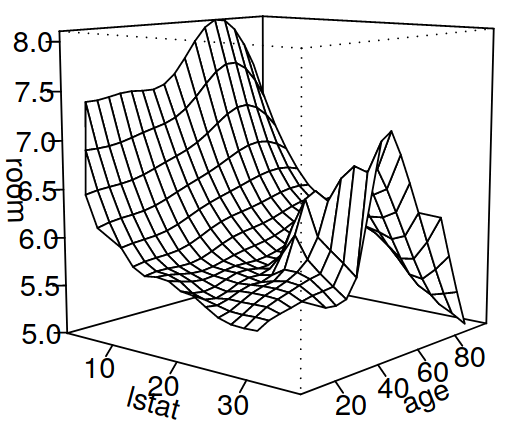
\includegraphics[width=0.6\textwidth]{boston_bivariate}
        \caption{Non-parametric fit of \texttt{ROOM} as a function of \texttt{LSTAT} and \texttt{AGE}.}
    \end{figure}
\end{example}

\pagebreak
\section{Splines}

Smoothing splines can be generalized to higher dimensions:
\begin{problem}{Smoothing splines for higher dimensions}{}
    \begin{equation*}
        \min_{\tilde m} \sum_{i=1}^n  \left( y_i - \tilde m*\boldsymbol x \right)^2 + \lambda \phi (\tilde m)
    \end{equation*}
    where (assuming that there are only $p=2$ predictors):
    \begin{equation*}
        \phi(f) = \int \int_{\mathbb R^2}
            \left( \frac{\partial^2 f(x_1, x_2)}{\partial x_1^2} \right)^2
            + 2 \left( \frac{\partial^2 f(x_1, x_2)}{\partial x_1 \partial x_2} \right)^2
            + \left( \frac{\partial^2 f(x_1, x_2)}{\partial x_2^2} \right)^2
            \, dx_1 \, dx_2
    \end{equation*}
    \tcblower
    The solution is a \iemph{thin plate spline}, a function of the form (for $p=2$):
    \begin{equation*}
        \tilde m (\boldsymbol x) = \beta_0 + \boldsymbol\beta^T \boldsymbol x
        + \sum_{i=1}^n \alpha_jh_i(\boldsymbol x)
    \end{equation*}
    where $h_i(\boldsymbol x) = \eta \left( \lVert \boldsymbol x - \boldsymbol x_i \rVert \right)$
    and $\eta(z) = z^2 \log(z)$.

    Basis is: $\{h_i(\boldsymbol x)\}_{i=1}^n$: as many elements as observations.

    \begin{note}
        High computational complexity: $O(n^3)$ for $p \geq 2$. Approximations
        with complexity $O(pn^2)$ are possible. We can reduce the number of
        knots.
    \end{note}
\end{problem}

\subsection{Tensor product splines}
Consider the case of $p=2$ explanatory variables $x$ and $z$.

Assume that basis of functions for expanding univariate functions depending on either
$x$ or $z$, have been determined:
\begin{equation*}
    f_X(x) = \sum_{j=1}^J \alpha_ja_j(x),\quad f_Z(z) = \sum_{h=1}^H \beta_hb_h(z)
\end{equation*}

Then, a \iemph{tensor product basis} for functions depending on both $x$ and $z$ is
defined as the collection of:
\begin{equation*}
    \left\{
        a_j(x) b_h(z) \mid j=1,\ldots,J,\, h=1,\ldots,H
    \right\}
\end{equation*}
that allows for expansions of the form:
\begin{equation*}
    f(x,z) = \mathlarger{\sum_{j=1}^J} \sum_{h=1}^H \gamma_{jh} a_j(x) b_h(z)
\end{equation*}

\begin{figure}[H]
    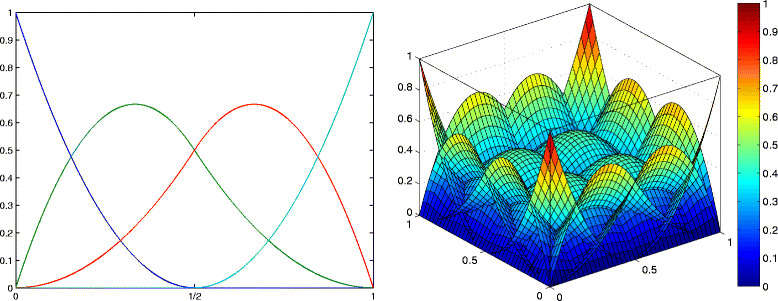
\includegraphics{2d_cubic_splines}
    \caption{1D and 2D cubic B-splines basis functions.}
    % https://www.researchgate.net/figure/1D-and-2D-quadratic-B-spline-basis-functions_fig1_270665031
\end{figure}

Fitting functions:
\begin{equation*}
    f(x,\,z) = \mathlarger{\sum_{j=1}^J} \sum_{h=1}^H \gamma_{jh} a_j(x) b_h(z) = \boldsymbol g(x,\,z)^T \boldsymbol\gamma
\end{equation*}

Penalty for tensor product splines (two penalty parameters):
\begin{align*}
    \phi(f) &= \int \int_{\mathbb R^2}
    \lambda_x \left( \frac{\partial^2 f(x,\,z)}{\partial x^2} \right)^2
    + \lambda_z \left( \frac{\partial^2 f(x,\,z)}{\partial z^2} \right)^2
    \, dx \, dz \\
            &= \lambda_x \boldsymbol \gamma^T \boldsymbol D_x \boldsymbol \gamma
            + \lambda_z \boldsymbol \gamma^T \boldsymbol D_z \boldsymbol \gamma
\end{align*}

\begin{problem}{Tensor product splines (p = 2)}{}
    \begin{equation*}
        \min_{\boldsymbol \gamma \in \mathds R^{J \times H}}
        \left(
            Y - \boldsymbol G\boldsymbol \gamma
        \right)^T
        \left(
            Y - \boldsymbol G\boldsymbol \gamma
        \right)
        + \lambda_x \boldsymbol \gamma^T \boldsymbol D_x \boldsymbol \gamma
        + \lambda_z \boldsymbol \gamma^T \boldsymbol D_z \boldsymbol \gamma
    \end{equation*}
    \tcblower
    \begin{note}
        \paragraph{Main drawback:} Exponential growth in basis functions as $p$ increases.
        So, we must reduce the number of basis per coordinate.
    \end{note}
\end{problem}

\pagebreak
\section{The curse of dimensionality}\index{curse of dimensionality}

Recall the problem introduced in \cref{sec:curse-of-dimensionality}. As explained
there, non-parametric estimation of the regression function is extremely difficult
when $p$ is large ($p \geq 4$). One way to solve this problem
is to use \emph{extremely} large sample sizes, (note that
for some problems having 842,000 observations in 10 dimensions is
equivalent to having 4 observations in 1 dimension).

For an exploratory variable in $\mathds R^p$, it can be proved that
the linear regression has $\text{AMSE}_0 = O(n^{-4/(p+4)})$.

The higher the dimension $p$ of explanatory variable, the lower the precision with which
the regression function is estimated.

There exist proposals, alternative to local polynomial regression or spline smoothing,
that overcome the curse of dimensionality:
Additive models and Projection pursuit are two of them that will be discussed in the
following sections.

\pagebreak
\section{Additive Models}

\begin{definition}{Additive Model}{additive-model}
    \begin{equation*}
        y_i = \alpha + \sum_{j=1}^p g_j(x_{ij}) + \epsilon_i
    \end{equation*}
    where $\mathds E(\epsilon_i) = 0$, $\text{Var}(\epsilon_i) = \sigma^2$ and
    $\mathds E(g_j(X_{j})) = 0$.

    Functions $g_j$ are called \emph{additive components} and must be estimated
    non-parametrically because no parametric model is specified for them.

    \tcblower

    The main assumption in this model is that the non-parametric univariate functions
    $g_j$ are combined additively to produce the non-parametric $p$-dimensional
    regression function.

    \begin{note}
        The additive model is halfway between the multiple linear regression model
        (which additively combines linear transformations of the explanatory variables: $\beta_jx_{ij}$)
        and the multiple non-parametric regression model.
    \end{note}
\end{definition}

\begin{example}{Boston housing data additive model}{}
    This is the same as in example~\ref{ex:boston1}, but using an additive model.
    \begin{figure}[H]
        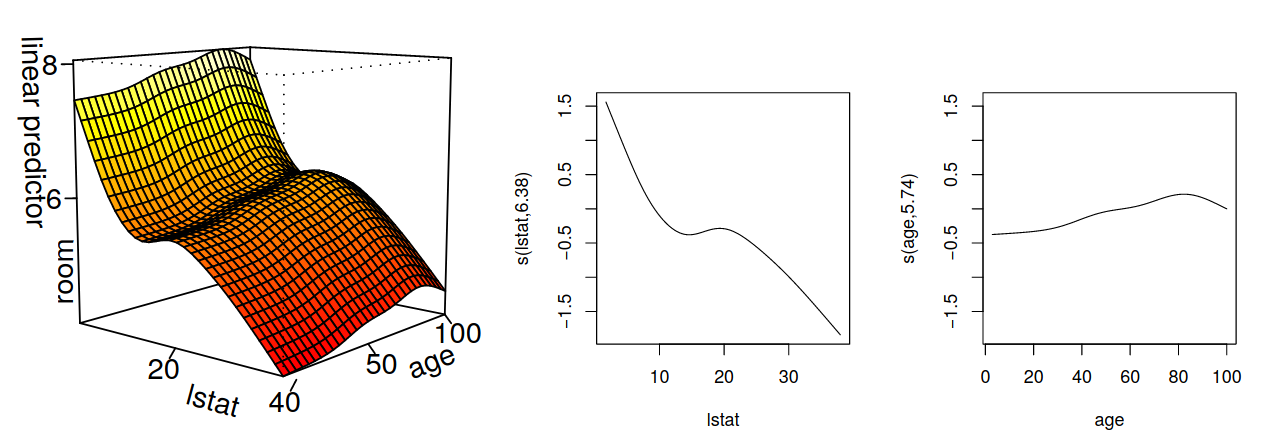
\includegraphics{additive}
        \caption{Non-parametric additive model of \texttt{ROOM} as a function of \texttt{LSTAT} and \texttt{AGE}.}
    \end{figure}

    \tcblower

    If we compare this model with the bivariate one, we can see that the additive model
    cannot pick up the local maximum located around $(\texttt{LSTAT},\, \texttt{AGE}) = (35,\, 50)$ because
    it is more rigid than the non-parametric bivariate model.

    \begin{note}
        The surface can be obtained by shifting the function $g_{LSTAT}$ over the function
        $g_{AGE}$ or vice versa and adding the mean of \texttt{ROOM}.
    \end{note}
\end{example}

\pagebreak
\subsection{Estimating the additive model}
Observe that $\mathds{E}(y_i) = \alpha$ since $\mathds{E}(\epsilon_i) = 0$
and $\mathds{E}(g_j(X_{j})) = 0$ (see~\ref{def:additive-model}).

Assume for a moment that the parameter $\alpha$ and all functions
$g_j$ are known except for $g_k$. Then $g_k$ could be estimated using
a non-parametric univariate smoother (i.e. local linear fit).
It would be enough to apply the smoother to data $(x_{ik},\, y_i^{(k)})$
where:
\begin{equation*}
    y_i^{(k)} = y_i - \alpha - \sum_{j \neq k} g_j(x_{ij})
\end{equation*}

This reasoning leads to the \emph{backfitting} algorithm to estimate
the additive model.

\begin{algorithm}{Backfitting algorithm}{backfitting}
    \begin{enumerate}
        \item Estimate $\alpha$ using the sample mean of $y_i$: $\hat \alpha = \frac{1}{n} \sum_{i=1}^n y_i$.
        \item Take an arbitrary function $\hat g_k = g_k^0$ as initial estimate of function $g_k$,
            for $k = 1,\dots,p$. (For instance, $g_k^0(x_{ik}) = \hat \beta_k x_{ik}$ where
            the coefficients $\hat \beta_k$ are estimated using the multiple linear regression model.)
        \item For $k = 1,\dots,p$:
            \begin{enumerate}
                \item Estimate $g_k$ using a non-parametric univariate smoother
                    to data $(x_{ik},\, y_i^{(k)})$ where:
                    \begin{equation*}
                        y_i^{(k)} = y_i - \alpha - \sum_{j \neq k} g_j(x_{ij})
                    \end{equation*}
            \end{enumerate}
        \item Repeat step 3 until convergence.
    \end{enumerate}
\end{algorithm}

\subsubsection{Basis functions}

Consider now the expansion of each function $g_j(x_j)$ in a basis function
(B-splines, for instance):
\begin{align*}
    m(\boldsymbol x) &= \alpha + \mathlarger{\sum_{j=1}^p} \sum_{h=1}^H \beta_j^h b_j^h(x_j) \\
        &= \alpha + \left(
            \boldsymbol b_1(x_1)^T, \ldots, \boldsymbol b_p(x_p)^T
        \right) \begin{pmatrix}
            \beta_1 \\
            \vdots \\
            \beta_p
        \end{pmatrix}
\end{align*}

Penalty term:
\begin{equation*}
    \Psi(m) = \sum_{j=1}^p \lambda_j \int_{\mathds R} \left( g_j'' (x_j) \right) dx_j
        = \sum_{j=1}^p \lambda_j \boldsymbol\beta_j^T \boldsymbol D_j \boldsymbol\beta_j
\end{equation*}

The, the GAM model is estimated as a penalized multiple linear regression model with
$1 + \sum_{j=1}^p H_j$ parameters.

The smoothing parameters $\lambda_1,\dots,\lambda_p$ are estimated using cross-validation
(LOOCV of GCV).

\section{Generalized Additive Models}

\begin{definition}{Generalized additive models (GAM)}{GAM}
    Additive models can be generalized similarly to generalized linear models
    (as seen in \ref{def:gnprm})

The r.v. $(Y; \boldsymbol X)$, with $\boldsymbol X = (X_1,\dots,X_p)$ has a distribution such
that:
\begin{equation*}
    (Y \mid \boldsymbol X) = (x_1,\dots,x_p) \sim f(y;\,m(x_1, \ldots, x_p),\,\psi)
\end{equation*}
where $m(x_1, \ldots, x_p) = \mathds{E}(Y \mid \boldsymbol X = (x_1,\dots,x_p))$ is a
smooth function of $(x_1,\dots,x_p)$ possible subject to certain constrains (e.g. non-negativity)
and $\psi$ represents other parameters (e.g. variance) not depending on $(x_1,\dots,x_p)$.

There exists an invertible \iemph{link function} $g$ such that:
\begin{equation*}
    \theta(x_1,\ldots,x_p) = g(m(x_1,\ldots,x_p)), \quad m(x_1,\ldots,x_p) = g^{-1}(\theta(x_1,\ldots,x_p))
\end{equation*}
where $\theta(x_1,\ldots,x_p)$ is a \iemph{smooth function} of $(x_1,\ldots,x_p)$ free of
constraints.
\tcblower
Alternatively, we can write:
\begin{equation*}
    (Y \mid \boldsymbol X = (x_1,\dots,x_p)) \sim f_2(y;\,\theta(x_1, \ldots, x_p),\,\psi)
    = f(y;\,g^{-1}(\theta(x_1, \ldots, x_p)),\,\psi)
\end{equation*}
\end{definition}

The non-parametric estimation of $\theta$ and $m$ by maximum local
likelihood suffers the effects of the \iemph{curse of dimensionality}.

A penalized maximum likelihood approach (with penalization for the
lack of smoothness of the estimated function) is also problematic
for moderate or large dimension $p$.

The possible solution is to use the \emph{Generalized Additive Model} (GAM):
\begin{equation*}
    \theta(x_1,\ldots,x_p) = \alpha + \sum_{j=1}^p g_j(x_j)
\end{equation*}

If the restriction that the functions $g_j$ are linear is added,
we obtain the \emph{Generalized Linear Model} (GLM).

\begin{note}
The GAM is halfway between the Generalized non-parametric multiple regression model
and the Generalized Linear Model.
\end{note}

\subsection{Generalized Additive Models Estimation}

The estimation of GAMs combines methods used to fit additive models with the
\iemph{IRWLS} algorithm (used to fit generalized linear models).

We replace each multiple linear regression fit by WLS is replaced
by the fitting of a weighted additive model (using backfitting
or penalized multiple linear regression, after a basis expansion)

This way, the final model is GAM instead of a GLM.

\subsection{Local scoring algorithm for logistic GAM}

\begin{enumerate}
    \item Compute starting values $\hat \alpha = \log \left( \frac{\bar y}{1-\bar y} \right)$
        where $\bar y$ is the sample proportion of ones, and set $\hat f_j = 0,\,\forall j$.
    \item Define $\hat \eta_i = \hat \alpha + \sum_{j=1}^p \hat f_j(x_{ij})$ and
        $\hat p_i = \frac{e^{\hat \eta_i}}{1+e^{\hat \eta_i}}$.
    Then Iterate:
        \begin{enumerate}
            \item Construct the working target variable $z_i = \hat \eta_i + \frac{y_i - \hat p_i}{\hat p_i(1-\hat p_i)}$.
            \item Construct weights $w_i = \hat p_i(1-\hat p_i)$.
            \item Fit a weighted additive model to the targets $z_i$ with
                exploratory variables $x_{ij}$ and weights $w_i$ using
                a weighted backfitting algorithm (or penalized basis expansions).

                This gives new estimates $\hat f_j,\,\forall j$.
        \end{enumerate}
        \item Repeat step 2 until the change in functions falls below a previously
            specified threshold.
\end{enumerate}

\pagebreak
\section{Semi-parametric models}

Sometimes some of the explanatory variables involved in the
definition of an additive model (or GAM)
affect the response variables linearly.

If this is known in advance, the GAM model can be reformulated
allowing some functions $g_j$ to be linear:
$g_j(x_j) = \beta_j x_j$.

Other possible modifications of the GAM model are:
\begin{itemize}
    \item non-parametrically estimating the combined effect of two (or more)
        explanatory variables. This includes for examples, replacing
        $g_j(x_j) + g_k(x_k)$ by $g_{jk}(x_j, x_k)$.
    \item Estimating the effect of a variable $x_j$ differently at each of the
        classes determined by another categorical variable $x_h$. There
        effects could be estimated linearly of non-parametrically.
\end{itemize}

Models incorporating this modifications to the GAM model are known as
\iemph{semi-parametric models}.

These models can be fitted using the function \texttt{gam} in the R package
\texttt{mgcv}. The \texttt{anova.gam} functions allows for testing between
nested GAM models.


% Functional Data Analysis
%! TEX root = ../000-main.tex
\part{Functional Data Analysis}

%! TEX root = ../000-main.tex
\chapter{Introduction to Functional Data Analysis (FDA)}
\chaptermark{FDA Intro.}

\section{An overview of FDA}

Observing and saving complete functions as the result of random
experiments is possible by the development of real-time
measurement instruments and data storage resources.

\begin{example}{}{}
	For patients involved in a clinical trial, the blood pressure
	is monitored in continuous-time during 24 hours
\end{example}

\begin{definition}{Functional data}{}
	Samples where a whole function is observed at each sampling unit
	are referred to as \iemph{Functional Data}.
	\tcblower
	Random functions are \iemph{Statistical atoms} in this case.
\end{definition}

\begin{figure}[H]
	\begin{tikzpicture}[
			every node/.style={rectangle, draw,rounded corners,inner sep=10pt},
		]
		\node (u) {Univariate};
		\node[right=of u] (m) {Multivariate};
		\node[right=of m] (f) {Functional};
		\draw[->,thick] (u) -- (m);
		\draw[->,thick] (m) -- (f);
	\end{tikzpicture}
	\caption{Evolution of Statistical Analysis}
\end{figure}

Functional data analysis (FDA) deals with the statistical description
and modeling of samples of \iemph{random functions}.

Functional data can also be obtained from standard random samples,
by the application of non-parametric curve estimation methods:
\begin{itemize}
	\item Non-parametric density estimation.
	\item Non-parametric regression.
	\item Non-parametric version of the GLM.
\end{itemize}

Kernel estimators, local polynomial regression, local likelihood,
spline smoothing and interpolations \dots

Many standard statistical techniques have been extended to
functional data:
\begin{itemize}
	\item \textbf{Exploratory data analysis} (location and scale measures, \dots).
	\item \textbf{Regression models} (lm, glm, non-parametric, \dots).
	\item \textbf{Multivariate Analysis} (PCA, MDS, Clustering, Depth measures, \dots).
	\item \textbf{Hypothesis testing}.
	\item \textbf{Time Series}, \textbf{Spatial Statistics}, \dots
\end{itemize}

Others methods are specific for this kind of data because they
exploit the nature of functions:
\begin{itemize}
	\item \textbf{Principal differential analysis} is a kind of principal component
	      analysis made on the derivatives of the observed functions,
	\item \textbf{Registration} is a pre-process step where a change of variable is done
	      in each observed function in order to make them as similar as
	      possible.
\end{itemize}

\paragraph{Software}
In R, the \texttt{fda} package provides a set of tools for functional data analysis.
There is also \texttt{fda.usc} among others.

\sectionmark{Concepts of FA for FDA}%
\section{Concepts of Functional Analysis useful in FDA}

\begin{definition}{Spatial dependence}
	When dealing with spatial data, the \iemph{spatial dependence} is
	the correlation between the values of a variable at two different
	locations in space.
\end{definition}

\pagebreak
\sectionmark{Formal definition}%
\section{Formal definition of functional data}%
\sectionmark{Formal definition}%

\begin{definition}{functional random variable}{frv}
	A random variable $\boldsymbol{\mathcal X}$ taking values in an infinite dimensional space (or
	functional space)
\end{definition}

\begin{definition}{functional data}{fd}
	An observation $\mathcal X$ of $\boldsymbol{\mathcal X}$ is called \iemph{functional data}.
	\tcblower

	Likewise a \iemph{functional data set} $\mathcal X_1,\ldots,\mathcal X_n$ is a collection of $n$
	observations of functional variables $\boldsymbol{\mathcal X_1}, \ldots, \boldsymbol{\mathcal X_n}$
	identically distributed as $\boldsymbol{\mathcal X}$.
\end{definition}

Let $T = [a,\,b] \subseteq \mathds R$, usually we work with functional data that are
elements of $L^2(T)$, the space of square integrable functions on $T$:
\begin{equation*}
	L^2(T) = \left\{ f : T \to \mathds R \,\middle|\, \int_a^b f^2(t) \,dt < \infty \right\}.
\end{equation*}

Smoothness of $\mathcal X$ as a function of $t \in T = [a,\, b]$ is implicitly assumed.

\begin{definition*}{Hilbert Space}{HS}
	A Hilbert space is a vector space endowed with an inner product.
\end{definition*}

\begin{definition}{Separable Hilbert Space}{}
	A separable Hilbert space is a Hilbert space that is separable as a metric space. That is,
	an infinite generalization of the usual Euclidean spaces in $\mathds R^p,\,p\in\mathds N^+$.
	\tcblower
	\begin{note}
		$L^2(T)$ is a separable Hilbert space with the inner product:
		\begin{equation*}
			\langle f, g \rangle = \int_T f(t) g(t) \,dt.
		\end{equation*}
	\end{note}
\end{definition}

\pagebreak
\subsection{Functional data and random processes}

\begin{definition}{Random process}{rp} (or \iemph{stochastic process})\index{random process}
	indexed by $T = [a,\,b] \subseteq \mathds R$
	is a random variable $\boldsymbol{\mathcal X}$ taking values in:
	\begin{equation*}
		L^2(T) = \left\{ f : T \to \mathds R \,\middle|\, \int_a^b f^2(t) \,dt < \infty \right\}.
	\end{equation*}
    \tcblower

    This is the same $L^2(T)$ as the one usually used for functional data.
\end{definition}

\begin{question*}{What is the difference between a functional data and a random process?}

	In random process analysis it is usually assumed that we can observe
    only \emph{one} realization of the process, while in functional data analysis
	it is always assumed that independent observations from the random
	process are available.
\end{question*}

% \section{Concepts of Functional Analysis useful in FDA}


%! TEX root = ../000-main.tex
\chapter{Observed functional data and its computational representation}
\chaptermark{Observed FD}

\section{Observing functional data in practice}

It is not possible to observe (sample) and/or to record (store)
a functional data $\mathcal X_i$ for all $t\in T=[a,\,b]$:
\begin{itemize}
	\item The measurement devices are only able to sample the phenomenon
	      only at discrete instants (even if the sample frequency is extremely high).
	\item Given that $T = [a,\,b]$ is an infinite set, saving all
	      $\mathcal X_i$ for all $t\in T$ would imply to use an infinite amount of memory.
\end{itemize}

In practice, $\mathcal X_i$ is sampled/recorded in a finite grid:
\begin{equation*}
	t_{i1} < \cdots < t_{im_i} \subset T
\end{equation*}
where $m_i$ is the number of samples. If $m_i$ is large enough,
the maximum difference between two consecutive samples
$\max_j\left\{t_{ij} - t_{i(j+1)}\right\}$ is small.

\begin{recap}{}{}
    \begin{itemize}
        \item In practice a functional data $\mathcal X$ is not fully observed.
            It is impossible to observe $\mathcal X(t)$ for all $t\in T$.
        \item Only a finite amount of values $\mathcal X(t_j)$ can be observed
            and registered, $t_j \in [A,\,B],\,j\in\mathds N$.

        \item The set of observed values is called the \emph{sample grid}.
        \item Moreover, the observation process can be affected by an observational noise.
    \end{itemize}
\end{recap}

This presents 4 scenarios, as depicted in \cref{fig:observed-fd-scenarios}:
\begin{figure}[H]
	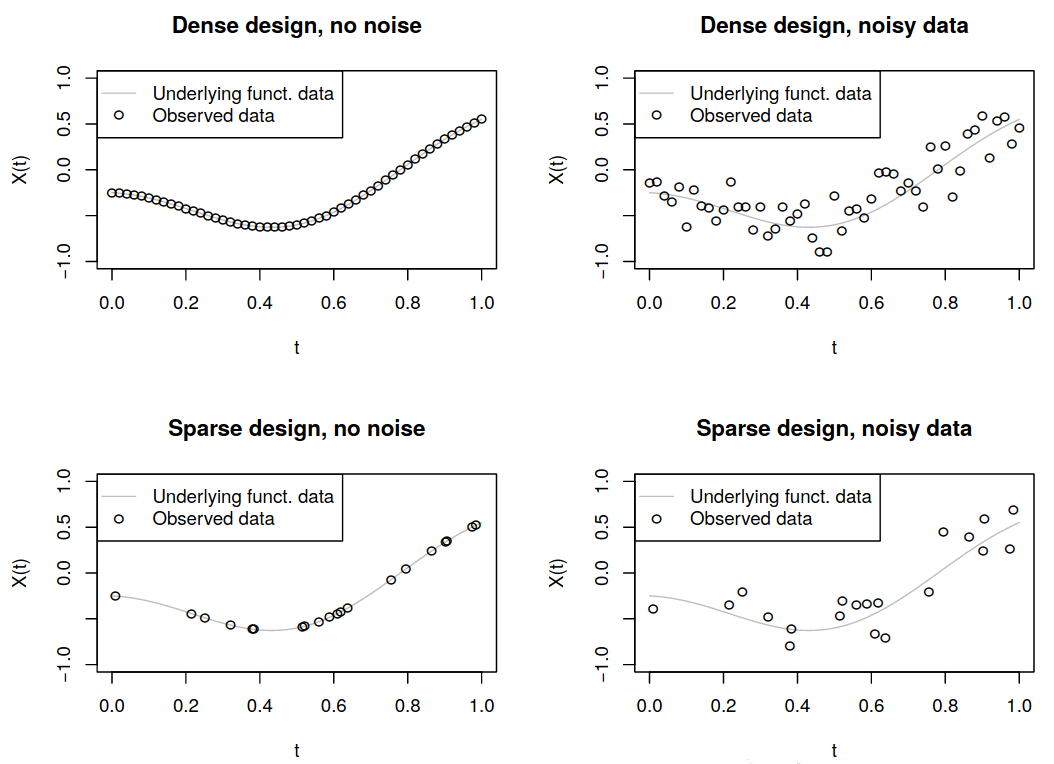
\includegraphics{observed-fd-scenarios}
	\caption{Example scenarios for the observation of functional data}
	\label{fig:observed-fd-scenarios}
\end{figure}

\subsection{Dense design}

\begin{definition}{Evenly Spaced Sampling}{}
	\begin{equation*}
		t_{j+1} - t_j = \delta = \frac{t_m - t_1}{m}
	\end{equation*}
\end{definition}

\subsection{Sparse design}

% TODO

\begin{definition}{Functional Data (practical definition)}{fdp}
	Multivariate data with an ordering on the dimensions.

	This definition implicitly assumes a common ordered design:
	\begin{equation*}
		t_1 < \cdots < t_m :  \mathcal X_i (t_j) + \varepsilon_{ij},\quad
		j=1,\ldots,m,\quad i=1,\ldots,n
	\end{equation*}
	\tcblower
	\begin{note}
		Ordering in the $m$ dimensions of the data is \emph{crucial},
		because it allows us to talk about \iemph{close dimensions}%
		\footnote{Close dimensions are more correlated than \iemph{distant dimensions}.}%
		.
	\end{note}
	\begin{note}
		This is an alternative way of saying that the functional data
		$\mathcal X_i$ are smooth functions.
	\end{note}
\end{definition}

\begin{question*}
	{Is FDA really different from Multivariate Analysis?}
	\begin{itemize}
		\item In Functional Data Analysis, the methods and procedures are
		      designed as if the functional data $\mathcal X_i(t),\,t\in T=[a,\,b]$
		      were available.
		\item Then the observed data $x_{ij}$ are used to estimate the required
		      elements.
		\item Finally, the outputs are displayed taking into account the functional
		      character of the objects of interest.
	\end{itemize}
\end{question*}



\pagebreak
\section[Representing functional data]{Representing functional data in a computer}

\subsection{Matrix representation}

\subsubsection{Common evenly spaced dense design}
Common evenly spaced (or not) dense design with no noisy data:
\begin{equation*}
	x_{ij} = \mathcal X_i(t_j),\quad j=1,\ldots,m,\quad i=1,\ldots,n
\end{equation*}
already have a good representation as a $n\times m$ matrix
$\boldsymbol X = \left(x_{ij}\right)_{n\times m}$.

If $\delta = t_{j+1} - t_j$ is small enough, many (if not all) the
required methods and procedures in FDA can be satisfactorily numerically
approximated using this matrix representation.

\subsubsection{Other situations}
For functional data with noisy data and/or sparse design, \iemph{smoothing
	methods} allows us to obtain a smooth estimation of the
underlying functional data with a common evenly spaced dense design. This
estimations can then be represented as a matrix.

\subsection{Basis-expansion representation}

Consider the square integrable Hilbert Space $L^2(T)$.
The inner product $\langle f, g\rangle = \int_T f(t)g(t)\,dt$ induces
a norm $\|f\| = \sqrt{\langle f, f\rangle}$ and a distance
between two functions $d(f, g)$:
\begin{equation*}
	d(f, g) = \lVert f - g \rVert = \sqrt{\langle f - g, f - g\rangle}
\end{equation*}

\begin{prop*}{}
	Any separable Hilbert space admits a countable orthonormal basis.
\end{prop*}

\begin{definition}{Countable Orthonormal basis}{}\index{countable orthonormal basis}\index{basis}

	A countable family $B = \{\phi_k\}_{k\in\mathds N},\, \phi_k\in{}H$ of functions
	that satisfies:
	\begin{alignat*}{2}
		\langle \phi_k, \phi_j\rangle        & = 0, \quad                                              & \forall & k,j \in \mathds N,\; k\neq j
		\tag{Orthogonality}                                                                                                                            \\
		\lVert \phi_k \rVert                 & = 1 \quad                                               & \forall & k \in \mathds N \tag{Normalization} \\[1em]
		\span\span\forall f\in L^2(T)\quad \exists \{c_k^f\}_{k\in\mathds N} \subset \mathds R \text{ s.t.}                                            \\
		\lim_{K\to\infty} \left\lVert
		f - \sum_{k=1}^{K} c_k^f \phi_k
		\right\rVert                         & = 0                                                                                                     \\
		\span\span\text{In fact, } c_k^f = \langle f,\, \phi_k\rangle                                                                                  \\
		f = \sum_{k=1}^{\infty} c_k^f \phi_k & = \sum_{k=1}^{\infty} \langle f,\, \phi_k\rangle \phi_k
		\tag{Completeness}
	\end{alignat*}
	\tcblower
	\begin{note}
		If $B$ satisfies only the last condition (\iemph{completeness}),
        it is called a basis of $L^2(T)$. (But it is not an \iemph{orthonormal basis})
	\end{note}
\end{definition}

\subsubsection{Finite basis-expansions for representing functional data}

For the orthonormal basis, when $K$ goes to infinity:
\begin{equation*}
    \lim_{K\to\infty} \left\lVert
    f - \sum_{k=1}^{K} c_k^f \phi_k
    \right\rVert \downarrow 0
\end{equation*}

Then the $K$-dimensional approximations (\iemph{finite basis-expansions})
\begin{equation*}
    f \approx = \sum_{k=1}^{K} \langle f,\, \phi_k\rangle \phi_k
\end{equation*}
are increasingly good approximations of $f$ as $K$ increases.

\begin{marker}
    Finite expansions in a given basis are a standard way to represent functional
    data.
\end{marker}

\subsubsection{Fourier basis}

A very convenient (before the computer age) example of
basis for the functional space $L^2(T),\,T=[a,\,b]$ is the \iemph{Fourier basis}:

\begin{definition}{Fourier Basis}{}\index{Fourier basis}
    Basis which elements are sine and cosine functions with
    increasing frequencies:
    \begin{align*}
        \text{Let } \omega = \frac{2\pi}{b-a}& \\
        B = \{&
            1/\sqrt{b-a},\\
              &\sqrt{2/(b-a)}\cos(\omega t),\,
            \sqrt{2/(b-a)}\sin(\omega t),\\
              &\ldots \\
              &\sqrt{2/(b-a)}\cos(\omega k t),\,
            \sqrt{2/(b-a)}\sin(\omega k t),\ldots\,
        \}
    \end{align*}
    \begin{note}
        \textbf{Inconvenient:} The representation of a function $f$ in $B$ is
        \emph{always} a periodic function in $T = [a,\,b]$, even if $f$ is not.
    \end{note}
    \begin{note}
        \iemph{B-spline bases} Are a non-orthogonal basis which are a
        good alternative to the Fourier basis. They consist of
        piecewise polynomials 
    \end{note}
\end{definition}

\section{Regularization in FDA}

\begin{definition}{Regularization}{}\index{regularization}
    Penalization of a function for \iemph{lack of smoothness}.
\end{definition}

In FDA, regularization is required in two different problems:
\begin{itemize}
    \item Transforming observed non-smooth data to functional smooth data.
    \item Estimating smooth functional parameters in functional models.
\end{itemize}

\subsection{Transforming observed data into functional smooth data}

Observed data:
\begin{equation*}
    x_{ij} = \mathcal X_i(t_j) + \varepsilon_{ij},\, j = 1,\ldots, m, i = 1,\ldots, n
\end{equation*}
$t_{j+1} - t_j = \delta = (t_m - t_1)/(m)$ with $m$ large.

$\varepsilon_{ij}$ are independent zero-mean random variables
(possibly with a common variance or even identically distributed).

Desired objects: $\mathcal X_i(t),\,t\in T = [a,\,b],\, i = 1,\ldots, n$.

More precisely, we want to have a computer valid representation of
$\mathcal X_i(t)$. One of:
\begin{itemize}
    \item \textbf{Matrix representation}
    \item \textbf{Basis-expansion representation}
\end{itemize}

Assume that a basis representation if desired using $\{\phi_k\}_{k=1,\ldots,K}$.

Let $\hat{\mathcal X}_i(t) = \sum_{k=1}^K c_{k}^{\mathcal X_i} \phi_k(t),\,t \in [a,\,b]$

The coefficients $c_1,\ldots,c_K$ are chosen as the solution of the problem:

\begin{problem}{}{}
    \begin{equation*}
        \min_{c_1,\ldots,c_K} 
        \sum_{j=1}^{n_j} \left(
            x_{ij} - \hat{\mathcal X}_i(t_{ij})
        \right)^2
        + \lambda
        \int_{a}^{b} \left(
            L(\mathcal X_i)(t)
        \right)^2\, dt
    \end{equation*}
    where $L$ is a \iemph{linear differential operator} (e.g. a derivative):
    $L(f) = \sum_{h=1}^H a_h f^{(h)}$.
\end{problem}

Penalization $L(f) = f^{(2)}$ is called \emph{second-order smoothing} and
is used to avoid \emph{oscillations} in the approximations (bumpy functions),
since:
\begin{equation*}
    \int_{a}^{b} \left(
        f^{(2)}(t)
    \right)^2\, dt
\end{equation*}
is a measure of the \iemph{total curvature} of the function $f$.

\begin{note}
    This penalization is associated with cubic splines bases (as we will show later).
\end{note}

\subsubsection{Estimating functional parameters}

In most cases, estimating a (regression) model for functional data
consists of finding a function (the model parameter is a whole function)

The estimation problem has an expression of this kind:
\begin{problem}{}{}
    \begin{equation*}
        \min_{f:[a,\,b] \to \mathds R} T(f; \mathcal X_1,\ldots,\mathcal X_n)
    \end{equation*}
\end{problem}

This is an infinite-dimensional problem (very difficult) and moreover,
there is no guarantee that the estimated functional parameter is a smooth 
function.

A feasible option is to look for the best parameter belonging to the space of functions spanned by
a finite subset of a basis of functions.

Then the problem becomes a finite-dimensional optimization problem.

In addition to that, a regularization term is added to the objective function
in order to have a smooth solution

Let $f(t) = \sum_{k=1}^K \beta_k B_k(t),\,t\in [a,\,b]$
The coefficients $\beta_k$ are chosen as the solution of the problem:
\begin{problem}{}{}
    \begin{equation*}
        \min_{\beta_1,\ldots,\beta_K} T(f; \mathcal X_1,\ldots,\mathcal X_n)
        + \lambda_T \int_{a}^{b} \left(
            L(f)(t)
        \right)^2\, dt
    \end{equation*}
\end{problem}
where $\lambda_T$ is a \iemph{smoothing parameter}.

\begin{note}
When estimating functional parameters, finite basis expansion is
the functional representation of choice.
\end{note}

% \section{Developments in bases of functions}
% \section{Smoothing: Kernel, Local Polynomials, Splines}
% \section{Registration and transformations of functional data}

%! TEX root = ../000-main.tex
\chapter{Exploratory analysis of functional data}
\chaptermark{Exploratory FDA}

\section{Introduction}
\begin{question}{What are we interested in?}{}
	\begin{itemize}
		\item \emph{Mean function}.
		\item \emph{Variation}.
		\item \emph{Covariation} between different values of the argument,
		      or between two different functional data.
		\item \emph{Depth measures} and \emph{outlier} detection.
	\end{itemize}
\end{question}

\subsection{Main parameters of a functional random variable}

\newcommand{\X}{{\boldsymbol{\chi}}}
\newcommand{\Y}{{\boldsymbol{\gamma}}}
Given two \iemph{functional random variables} $\X$ and $\Y$:
\begin{align*}
	\mu(t)        & = \mathds E(\X(t)) \tag{Mean function}                                                                                                       \\
	\sigma^2(t)   & = \text{Var}(\X(t)) = \mathds E\left[
		\X(t)^2
	\right] - \mu(t)^2 \tag{Variance function}                                                                                                                   \\
	\sigma(t,\,u) & = c(t,\,u) = \mathds E\left[
		\X(t)\,\Y(u)
	\right] - \mu(t)\,\mu(u) \tag{Covariance function}                                                                                                           \\
	r(t,\,u)      & = \text{Cor}(\X(t),\,\X(u)) =
	\frac{\text{Cov}(\X(t),\,\X(u))}{\sqrt{\text{Var}(\X(t))\,\text{Var}(\X(u))}}
	\tag{Correlation function}                                                                                                                                   \\
	C_c(t,\,u)    & = \text{Cov}(\X(t),\,\Y(u)) = \mathds E\left[ \X(t)\,\Y(u) \right] - \mu_\X(t)\,\mu_\Y(u) \tag{Cross-covariance function}                    \\
	r_c(t,\,u)    & = \text{Cor}(\X(t),\,\Y(u)) = \frac{\text{Cov}(\X(t),\,\Y(u))}{\sqrt{\text{Var}(\X(t))\,\text{Var}(\Y(u))}} \tag{Cross-correlation function}
\end{align*}

\section{Descriptive Analysis}

Given a functional data set $\X = (\chi_1,\, \gamma_1),\, \dots,\, (\chi_n,\, \gamma_n)$, iid
from $(\X,\,\Y)$, the \emph{natural estimators} of their main parameters are:

\begin{definition}{Mean}{}
	\begin{equation*}
		\bar \chi (t) = \frac{1}{n} \sum_{i=1}^n \chi_i(t) \tag{mean}
	\end{equation*}
\end{definition}
\begin{definition}{Variance}{}
	\begin{equation*}
		\hat \sigma^2(t) = \frac{1}{n-1} \sum_{i=1}^n \left( \chi_i(t) - \bar \chi(t) \right)^2 \tag{variance}
	\end{equation*}
\end{definition}
\begin{definition}{Covariance}{}\index{covariance}
	\begin{equation*}
		\hat c(t,\,u) = \frac{1}{n-1} \sum_{i=1}^n \left( \chi_i(t) - \bar \chi(t) \right) \left( \gamma_i(u) - \bar \gamma(u) \right) \tag{covariance}
	\end{equation*}
\end{definition}
\begin{definition}{Correlation}{}\index{correlation}
	\begin{equation*}
		\hat r(t,\,u) = \frac{\hat c(t,\,u)}{\sqrt{\hat \sigma^2(t)\,\hat \sigma^2(u)}} \tag{correlation}
	\end{equation*}
\end{definition}
\begin{definition}{Cross-covariance}{}\index{cross-covariance}
	\begin{equation*}
		\hat C_c(t,\,u) = \frac{1}{n-1} \sum_{i=1}^n \left( \chi_i(t) - \bar \chi(t) \right) \left( \gamma_i(u) - \bar \gamma(u) \right) \tag{cross-covariance}
	\end{equation*}
\end{definition}
\begin{definition}{Cross-correlation}{}\index{cross-correlation}
	\begin{equation*}
		\hat r_c(t,\,u) = \frac{\hat C_c(t,\,u)}{\sqrt{\hat \sigma_\chi^2(t)\,\hat \sigma_\gamma^2(u)}} \tag{cross-correlation}
	\end{equation*}
\end{definition}


% \section{Location and dispersion statistics}
\pagebreak
\section{Depth measurements}\index{depth measurements}

\begin{definition}{$\alpha$-trimmed mean}
    We remove from the data set the $\alpha/2$ lowest data
    and the $\alpha/2$ largest data, and compute
    the mean of the remaining data.
    \tcblower
    \begin{note}
        The aim is to remove the outliers.
    \end{note}
\end{definition}

\begin{definition}{Data Depth}{}
    a measure of how deep a data point is in the sample.

    They allow for centrality measures alternative to the mean, trying
    to generalize the median and the trimmed-mean
    of a univariate dataset.

    \tcblower

    \begin{note}
        In univariate data, the \emph{median} would typically be the deepest point
        of a cloud of points.
    \end{note}
\end{definition}

\subsection{Depth measure for univariate data}

\begin{definition}{Median depth}{}\index{depth measurements!median}

Given a univariate data set $x_1,\, \dots,\, x_n$, let
\begin{equation*}
    F_n(x) = \frac{\#\{x_i: x_i \leq x\}}{n} \tag{Empirical distribution function}
\end{equation*}
be the empirical distribution function of the data set. A \emph{depth measure} can
be defined as:
\begin{equation*}
    D(x_i) = \min\left\{ F_n(x_i),\, 1 - F_n(x_i) \right\} \tag{depth measure}
\end{equation*}
\end{definition}

\subsection{Depth measurements for multivariate data}

Different depth notions have been proposed for multivariate data:
\begin{itemize}
    \item Tukey (halfspace) depth, Simplical depth, convex hull peeling depth, etc.
\end{itemize}

\subsection{Depth measures for functional data}

\begin{definition}{Functional Depth}{}
    How deep a functional data is in the functional data set.

    Different functional depth notions have been proposed:
    \begin{itemize}
        \item Integration over the argument of univariate depth measures.
        \item Extensions of multivariate depths.
        \item Modal depth.
    \end{itemize}
    \tcblower
    Depth measures are useful to define \emph{robust location} and \emph{dispersion} measures,
    as well as \emph{classification} and \emph{outlier detection}.
\end{definition}

\subsubsection{Functional Depths based on univariate depth measures}

\begin{definition}{Fraiman-Muñiz Integrated Functional Depth}{}\index{FM}

Let $\chi_1,\, \dots,\, \chi_n$ be a functional data set defined over
$T = [a,\,b]$.

For a fixed $t \in T$, $\chi_1(t),\, \dots,\, \chi_n(t)$ is a univariate sample,
and associated to it there is a univariate depth measure $D(x)$

Let $D(\chi_i(t))$ be univariate depth measure of $\chi_i$ at $t$.
The \iemph{Fraiman-Muñiz} (FM) integrated functional depth measure of
$\chi_i$ is defined as:
\begin{equation*}
    D(\chi_i) = \int_a^b D(\chi_i(t)) \, dt \tag{FM depth}
\end{equation*}
\tcblower
\begin{note}
    Other alternative univariate depth measures can be used to define \iemph{integrated depths},
    apart from $D(x) = \min\left\{ F_n(x),\, 1 - F_n(x) \right\}$.
\end{note}
\begin{note}
    In addition to integrated depths, there are other ways to define functional depths.
\end{note}
\end{definition}

\subsubsection{Modal Depth}\index{modal depth}

\begin{question*}{
    Given a functional data $x_i$, how densely surrounded is it by other data in the 
    functional data set?
}
\end{question*}

\begin{definition}{Functional Modal Depth}{} the functional data most densely
    surrounded by other data points.

    Given a metric or a semi-metric $d(\cdot,\cdot)$ between functions, for
    fixed $h > 0$, the \iemph{$h$-depth} is defined as:
    \begin{equation*}
        D_h(x_i) = \sum_{j\neq i} \frac{1}{h} K\left( \frac{d(x_i,\,x_j)}{h} \right) \tag{$h$-depth}
    \end{equation*}
    where $K$ is a \emph{kernel function}%
    \footnote{a unimodal symmetric univariate density function}, typically the
    standard normal density.
    \tcblower
    The \emph{tuning parameter} $h$ is selected by default as the 15\%-quantile of
    the distances between the data points $d(x_j,\,x_k),\;j\neq k$.
\end{definition}

\subsection{From functional depth to descriptive tools}\index{trimmed mean/variance}

\begin{definition}{Functional Descriptive Tools}{}
    \begin{itemize}
        \item \textbf{Median}: the deepest function.
        \item \textbf{$\alpha$-trimmed mean}: the mean of the
            $(1-\alpha)\times n$ deepest functional data.
        \item \textbf{$\alpha$-trimmed variance}: the variance of the
            $(1-\alpha)\times n$ deepest functional data.
        \item \textbf{Outlier detection}: The least deep functional observations
            could be considered as outliers.
    \end{itemize}
    \begin{note}
        Functional outliers can appear when \emph{studying derivatives}, even if they are deep among
        the observed functions (with no derivatives).
    \end{note}
\end{definition}

% \section{Outliers detection}

%! TEX root = ../000-main.tex
\chapter{Dimensionality reduction in Functional Data Analysis}
\chaptermark{FDA Dim. red.}
% \marginpar{FDA 4.a}

\section{Introduction}
We observe $n$ functions $\chi_1,\, \dots,\, \chi_n$. In general,
they belong to an infinite-dimensional functional space:
$\{f: T \to \mathds R\},\,T = [a, b]$.
\begin{problem}{Dimensionality reduction}{}(in FDA)

Looking for a low dimensional configuration $X$
(an $n \times q$ matrix, $n < q$, with rows $x_i,\,i=1,\dots,n$) such that
and an application $\rho$ from $\mathds R^q$ to the functional space such
that $\rho(x_i)$ is close (in some sense) to the observed $\chi_i$ for all $i$.

\tcblower

Functional principal component analysis (\emph{FPCA}) and
Multidimensional scaling (\emph{MDS}) are two examples of dimensionality reduction methods.

% \tcbline

\begin{note}
	Usually, for visualization purposes, $q=2$ or $q=3$.
\end{note}
\end{problem}

\pagebreak
\section[Functional PCA]{Functional Principal Component Analysis (FPCA)}
\index{Functional PCA}\index{FPCA}

Consider the random function $\boldsymbol \chi : \mathcal T = [a, b] \to \mathds R$,
with $\mathds E [\boldsymbol \chi] = \mu(t),\, \forall t \in \mathcal T$ and
$\mathds E \left[ \int_a^b \left( \boldsymbol \chi(t) - \mu(t) \right)^2 \right] < \infty$.

\begin{problem}{FPCA}{FPCA}
Find orthonormal non-random functions $u_1,\, \dots,\, u_K$ from $\mathcal T$ to $\mathds R$,
minimizing:
\begin{equation*}
	\min_{u_1,\, \dots,\, u_K} \mathds E \left[
		\left\lVert
		\boldsymbol \chi - \mu - \sum_{j=1}^K \left\langle
		\boldsymbol \chi - \mu, u_j
		\right\rangle u_j
		\right\rVert^2
		\right]
\end{equation*}
\end{problem}

\begin{definition}{Low dimensional representation of $\boldsymbol \chi$}{}
	\begin{equation*}
		\boldsymbol \chi \approx \mu + \sum_{j=1}^K \left\langle
		\boldsymbol \chi - \mu, u_j
		\right\rangle u_j = \mu + \sum_{j=1}^K Z_j u_j
	\end{equation*}

	Once the functions $u_1,\, \dots,\, u_K$ have been determined, $\boldsymbol \chi(t),\,t\in[a,\,b]$
	is represented by the vector $Z = (Z_1,\, \dots,\, Z_K),\, Z_j = \left\langle
		\boldsymbol \chi - \mu, u_j
		\right\rangle$.
\end{definition}

\begin{definition}{Covariance Operator}{}

	Let $C(t,\,u) = \text{Cov} \left( \boldsymbol \chi(t),\, \boldsymbol \chi(u) \right)$ be
	the \iemph{covariance function} of $\boldsymbol \chi$.

	Associated to $C(t,\,u)$ is the \iemph{covariance operator} $\Gamma$:
	\begin{alignat*}{2}
		\Gamma : L^2(\mathcal T) & \to L^2(\mathcal T) &             &                                                   \\
		f                        & \mapsto \Gamma(f) : & \mathcal  T & \to \mathds R                                     \\
		                         &                     & t           & \mapsto \Gamma(f)(t) = \int_T C(t,\,u) f(u) \, du
	\end{alignat*}

	Let $\lambda_j,\,\psi_j$ be the eigenvalues and eigenfunctions of the
	covariance operator $\Gamma$:
	\begin{equation*}
		\Gamma(\psi_j) = \lambda_j \psi_j,\,j \geq 1
	\end{equation*}
\end{definition}

\subsection{FPCA and Karhunen-Loève expansion}

\begin{definition}{Karhunen-Loève expansion}{}

	Assuming $\mathds E \left[ \int_a^b \left( \boldsymbol \chi(t) - \mu(t) \right)^2 \right]
		= \mathds E \left[ \left\lVert \boldsymbol \chi - \mu \right\rVert^2 \right] < \infty$,
	the random function $\boldsymbol \chi(t)$ can be expanded as:
	\begin{equation*}
		\boldsymbol \chi(t) = \mu(t) + \sum_{j=1}^\infty Z_j\psi_j(t)
	\end{equation*}
	known as the \iemph{Karhunen-Loève expansion} of $\boldsymbol \chi$, where:
	\begin{equation*}
		Z_j = \left\langle \boldsymbol \chi - \mu,\, \psi_j \right\rangle,\,j \geq 1
	\end{equation*}
	is a sequence of random variables with \emph{mean zero} (${\mathds E[Z_j] = 0}$)
	and variance $\lambda_j$ (${\mathds E[Z_j^2] = \lambda_j}$)
	that are \emph{uncorrelated} (${\mathds E[Z_j Z_h] = 0},\,j \neq h$).

	\tcblower

	\begin{note}
		When the random function $\boldsymbol \chi$ is a Gaussian, then $Z_j$ are
		independent Gaussian random variables.
		\tcbline
		Moreover: $\mathds E \left[ \int_a^b \left( \boldsymbol \chi(t) - \mu(t) \right)^2 \right]
			= \mathds E \left[ \left\lVert \boldsymbol \chi - \mu \right\rVert^2 \right]
			= \sum_{j=1}^\infty \lambda_j$.
	\end{note}
\end{definition}

\begin{prop}{}{}
	Assuming $\lambda_j > \lambda_{j+1},\,\forall j \geq 1$ and fixing an integer $K$,
    the orthonormal basis $u_1,\, \dots,\, u_K$ solving the FPCA problem (\ref{problem:FPCA}) is
	formed by the first $K$ eigenfunctions $\psi_1,\, \dots,\, \psi_K$ of the covariance
	operator $\Gamma$. And the minimum is $\sum_{j\geq K+1} \lambda_j$.

    \tcblower

	\begin{marker}
		That is, the \emph{Karhunen-Loève expansion} of $\boldsymbol \chi - \mu$,
		truncated at the first $K$ terms gives the \emph{best $K$-dimensional approximation}
		to $\boldsymbol \chi - \mu$ in the sense of the mean square error.
	\end{marker}
\end{prop}

\subsection{Sampling version of FPCA}

The sampling (or empirical) version of the previous
results is obtained when replacing the covariance function of $\boldsymbol \chi$
by the \iemph{empirical covariance function}.

\begin{definition}{Empirical covariance function}{}

    Let $\chi_1,\, \dots,\, \chi_n$ be $n$ iid random functions on $L^2(\mathcal T)$
    having the same distribution as $\boldsymbol \chi$. The \emph{empirical covariance function}
    is:
    \begin{equation*}
        \hat C(t,\,u) = \frac{1}{n} \sum_{i=1}^n \left(
            \chi_i(t) - \hat \chi(t)
        \right)\cdot \left(
            \chi_i(u) - \hat \chi(u)
        \right)
    \end{equation*}
    forall $t,\,u \in \mathcal T = [a,\,b]$ where $\hat \chi$ is the \emph{sample mean function}:
    \begin{equation*}
        \hat \chi(t) = \frac{1}{n} \sum_{i=1}^n \chi_i(t)
    \end{equation*}

    \tcblower

    In practice, the eigensystem of the operator with kernel $\hat C(t,\,u)$ is
    obtained by \emph{matrix diagonalization}:
    \begin{equation*}
        \chi_i(t) \approx \hat \chi(t) + \sum_{j=1}^K \hat Z_{ij} \hat \psi_j(t),\,t \in \mathcal T,\,i=1,\, \dots,\, n
    \end{equation*}

\end{definition}

\subsection{Interpreting principal functions}
\begin{itemize}
    \item \emph{Mean function}: $\bar \chi$ represents what is common to all the data.
    \item \emph{Centered functions}: $\chi_i - \bar \chi$ account for individual differences.
    \item \emph{Principal functions}: summarize what is common in the way individuals are
        diverse. They represent the \emph{main variation modes} of the observed functions
        around the mean function.
    \item Graphical representation:
        \begin{itemize}
            \item PC k vs PC j scores.
            \item Mean function \textpm PC j (times a constant). The standard.
            \item Curves with \emph{Median and extreme scores in PC j}
                (alternative graphic proposed by Jones and Rice (1992)).
        \end{itemize}
\end{itemize}

\subsubsection{Numerical computation of sampling FPCA}

\begin{algorithm}{Numerical computation of sampling FPCA}{}
    proposed by Kneip and Utikal 2001

    Let us assume that a set of $n$ independent copies of $\boldsymbol \chi$ have
    been observed in a common fine grid in $T$:
    \begin{equation*}
        \chi_i(t_h),\,h=1,\, \dots,\, H,\,i=1,\, \dots,\, n
    \end{equation*}

    Let $\chi_i^c(t_h)$ be the centered observations.

    Let $M$ be the $n \times n$ matrix with element ($i,\,j$) equal to
    \begin{equation*}
        \left\langle \chi_i^c,\, \chi_j^c \right\rangle = \int_a^b \chi_i^c(t) \chi_j^c(t) \,dt
    \end{equation*}

    The eigenvalues of $M$, say $\hat\lambda_r,\,r=1,\, \dots,\, n$ coincide with
    the non-null eigenvalues of the sampling covariance operator $\hat C$ with
    kernel $\hat c(t,\,u)$.

    Let $(p_{1i},\, \dots,\, p_{ni})$ be the $i$-th eigenvectors of $M$. Then
    the $r$-th eigenfunction of the sampling covariance operator $\hat C$ is
    \begin{equation*}
        \hat e_r(t) = \hat \lambda_r \sum_{i=1}^n p_{ri} \chi_i^c(t)
    \end{equation*}

    In practice, matrix $M$ is not computable.

    Let $\hat M$ be the $n \times n$ matrix whose elements
    are numerical approximations of those of $M$:
    \begin{equation*}
        \hat M_{ij} = \sum_{h=2}^H \frac{\chi_i^c(t_h) \chi_j^c(t_h) + \chi_i^c(t_{h-1}) \chi_j^c(t_{h-1})}{2}
            (t_h - t_{h-1})
            \approx \int_a^b \chi_i^c(t) \chi_j^c(t) \,dt = M_{ij}
    \end{equation*}

    The eigensystem of $\hat M$ is used for approximating that of the sampling covariance operator $\hat C$.
\end{algorithm}\index{eigensystem}

\begin{algorithm}{Numerical computation of sampling FPCA}{}Using B-spline basis
    (Ramsey and Silverman 2005)

    Let $B_1(t),\, \dots,\, B_K(t)$ basis and express $\chi_i^c(t)$ as a linear combination of
    this basis:
    \begin{equation*}
        \hat \chi_i^c(t) \approx \sum_{k=1}^K \alpha_{ik} B_k(t),\,t \in T \implies
            \hat\chi_i^c \approx \alpha_i^T B
    \end{equation*}
    where $\alpha_i = (\alpha_{i1},\, \dots,\, \alpha_{iK})^T$ and $B = (B_1,\, \dots,\, B_K)$.

    Then
    \begin{equation*}
        \hat c(t,\,u) \approx \frac{1}{n} \sum_{i=1}^n \left(
            \alpha_i^T B(t) B(u)^T \alpha_i
        \right)
    \end{equation*}

    For a generic $f \in L^2(T)$, let $\beta^T B\approx f$ be the expression of $f$
    in the B-spline basis. Then:
    \begin{equation*}
        \lVert f \rVert^2 = \beta^T \Phi \beta \quad
        \Phi_{hl} = \mathlarger{\int_a^b} \int_a^b B_h(t) B_l(u) \,du \,dt
    \end{equation*}

    It can be proven that the first eigenfunction is also the solution of:
    \begin{equation*}
        \max_{f:\lVert f \rVert = 1} \widehat{\text{Var}} \left( \langle \boldsymbol \chi,\, f \rangle \right)
    \end{equation*}

    \begin{align*}
        \widehat{\text{Var}} \left( \langle \boldsymbol \chi,\, f \rangle \right)
        &= \langle\hat C(f),\, f \rangle
        = \mathlarger{\int_a^b} \left( \int_a^b \hat c(t,\,u) f(u) \,du \right)f(t) \,dt \\
        &\approx \mathlarger{\int_a^b} \left( \int_a^b \frac{1}{n} \sum_{i=1}^n \left(
            \alpha_i^T B(t) B(u)^T \alpha_i
        \right) \beta^T B(u) \,du \right) B(t)^T \beta \,dt \\
        &= \beta^T \left(\mathlarger{ \int_a^b }
        \int_a^b B(u) \left(
            \frac{1}{n} \sum_{i=1}^n \alpha_i^T B(t) B(u)^T \alpha_i
        \right) B(t)^T \,du \,dt \right) \beta \\
        &= \beta^T \hat \Psi \beta
    \end{align*}
    Then, $\max_{f:\lVert f \rVert = 1} \widehat{\text{Var}} \left( \langle \boldsymbol \chi,\, f \rangle \right)$
    is almost equivalent to:
    \begin{equation*}
        \max_{\beta\in\mathds R^K : \beta^T\Phi\beta = 1} \beta^T \hat \Psi \beta
        \iff
        \max_{\beta\in\mathds R^K : \left( \Phi^{1/2}\beta \right)^T \left( \Phi^{1/2}\beta \right) = 1}
            \left( \Phi^{1/2}\beta \right)^T
            \left( \Phi^{-1/2} \hat \Psi \Phi^{-1/2} \right)
            \left( \Phi^{1/2}\beta \right)
    \end{equation*}
    and the problem reduces to the \emph{diagonalization of $\Phi^{-1/2} \hat \Psi \Phi^{-1/2}$}.
\end{algorithm}

\begin{definition}{Sparse functional data}{}\index{sparse functional data}

    The observations are
    \begin{equation*}
        \chi_i(t_{ij}),\, h=1,\, \dots,\, m_i,\, i=1,\, \dots,\, n
    \end{equation*}
    where $m_i$ is the number of observations of the $i$-th individual.
    \begin{itemize}
        \item The number of observations $m_i$ for individual $i$ is small.
        \item Different individuals have different number of observations.
        \item The points $t_{ij}$ are not necessarily the same for all individuals.
    \end{itemize}

    Implemented in function \emph{\texttt{PACE} Principal Analysis by Conditional
    Expectation} in the R library \emph{fdapace}.
\end{definition}

\sectionmark{MDS}%
\section{Multidimensional Scaling for functional data}%

\begin{recap}{MDS}{}\index{Functional MDS}
MDS is a dimensionality reduction technique based on \emph{inter-individuals distances}.

Let $d_{ij} \geq 0$ be the dissimilarity between individuals $i$ and $j$.

It is assumed that $d_{ij} = d_{ji}$ and $d_{ii} = 0$.

We look for a $n \times q$ matrix $X\, (q \leq n)$ such that
the Euclidean distance between individuals $i$ and $j$ rows of $X$ is
as close as possible to $d_{ij}$.

$X$ can be chosen with orthogonal columns.

The columns of $X$ are called \emph{principal coordinates}.

\tcbline
Relation between PCA and MDS:
\begin{itemize}
    \item Let $X$ be a $n \times q$ data matrix.
    \item $d_{ji}$ be the Euclidean distance between rows $i$ and $j$ of $X$.
    \item Then $\tilde X_q\;(q \leq p)$ coincides with the matrix of the first
        $q$ principal coordinates of $X$.
\end{itemize}
\end{recap}

\begin{definition}{Functional MDS}{}
    %
    % Distance: $d(x,\,y) = 0 \iff x = y$ and $d(x,\,y) \leq d(x,\,z) + d(z,\,y)$.
    % Semi-metric: $d(x,\,x) = 0$ and $d(x,\,y) \leq d(x,\,z) + d(z,\,y)$.
    %
    When working with functions, \iemph{semi-metrics} (def~\ref{def:metric}) are used (i.e. two
    functions that are different in only one point are essentially the same)
\end{definition}

\begin{example}{Semi-metrics in $F = \{\chi : [a,\,b] \to \mathds R\}$}{}
    the set of functions defined on $T = [a,\,b]$:

    $L2$-distance between derivatives:
    \begin{equation*}
        d_r^{deriv}(\chi,\,\gamma) = \sqrt{
            \int_a^b \left(
                \chi^{(r)}(t) - \gamma^{(r)}(t)
            \right)^2 \,dt
        }
    \end{equation*}

    $L2$-distance in the first $q$ functional principal components:
    \begin{equation*}
        d_q^{PCA}(\chi,\,\gamma) = \sqrt{
            \sum_{i=1}^q \left(
                \psi_k^\chi - \psi_k^\gamma
            \right)^2
        } = \sqrt{
            \sum_{i=1}^q \left(
                \int_a^b \left[
                    \chi(t) - \gamma(t)
                \right] e_k(t) \,dt
            \right)^2
        }
    \end{equation*}
\end{example}

\sectionmark{Density functions}%
\section{Dimensionality reduction when data are density functions}

A particular case of functional data is the case of \iemph{density functions}.

The functional space is:
\begin{equation*}
    \mathcal F(I) = \{
        f : I \to \mathds R \mid f(x) \geq 0,\, \int_I f(x) \,dx = 1
    \}
\end{equation*}
where $I = [a,\,b] \subseteq \mathds R$.

Density functions share some features with \iemph{compositional data}
($D$-dimensional, non-negative data with constant sum).
Densities are in fact infinite dimensional compositional data.

% TODO

% %! TEX root = ../000-main.tex
\chapter{Regression with functional data as explanatory or response variable}

\section{Scalar response and functional regressor}
\section{Functional response}

%! TEX root = ../000-main.tex
\chapter{Applications: FDA in Demography}


% Interpretable Machine Learning
%! TEX root = ../000-main.tex
\part{Interpretable Machine Learning}

%! TEX root = ../000-main.tex
\chapter{Introduction to interpretability in machine learning}
\chaptermark{IML introduction}

\section{Model interpretability and variable relevance}

In a stimulating and provocative paper, Breiman (2001)
% TODO: cite
shook the
statistical community by making it to be aware that traditional
Statistics was no longer the only way to learn from data:
\begin{itemize}
	\item \emph{Data modelling culture} (traditional statistics):
	      \begin{itemize}
		      \item Linear regression, logistic regression, additive models, etc.
		      \item They allow to interpret how the response variable is associated with
		            the input variables: \iemph{Transparent models}.
	      \end{itemize}
	\item \emph{Algorithmic Modeling Culture} (machine learning):
	      \begin{itemize}
		      \item Decision trees, neural networks, support vector machines, etc.
		      \item They have extremely good predictive accuracy, and they usually outperform
		            in this criterion statistical models.
		      \item However, they have low interpretability: \iemph{Black-box models}.
	      \end{itemize}
\end{itemize}

From that it follows an apparent dichotomy: \iemph{predictive capacity} versus \iemph{interpretability}.

Breiman claimed for procedures allowing better interpretation of the algorithmic models
results, without giving up their predictive ability.

Machine learning community has been worried about interpretability:
\begin{quote}
	If the users do not trust a model or a prediction, they will not use it.

	\emph{Ribeiro, Singh and Guestrin (2016)}
\end{quote}

In 2018, the General Data Protection Regulation (GDPR) of the European Union
established users' right to explanation: ``When an algorithmic decision
significantly affects a user, he or she has the right to ask for an explanation
of such decision''.

A powerful research line has been developed:
\iemph{Interpretable Machine Learning} (\iemph{IML}) and
\iemph{eXplainable Artificial Intelligence} (\iemph{XAI}).

There are several review papers on this topic.
Barredo-Arrieta et al. (2020) is one of the most
recent and extensive ones. % TODO: cite properly
Also three monographs: Molnar (2019), Biecek and Burzykowski (2021), and
Masís (2021).

There are also many functions and packages in both R and Python.

\section{IML/XAI concepts}

\begin{note}
	The \emph{accuracy} of predictions is no longer the only criterion to evaluate
	the quality of a prediction algorithm.
\end{note}

Desirable properties for predictive models:
\begin{itemize}
	\item \iemph{transparency}
	\item \iemph{interpretability}
	\item \iemph{explainability}
\end{itemize}

However, these concepts are not well defined and are difficult to measure:
\begin{itemize}
	\item Lipton 2018: ``The term \emph{interpretability} is ill-defined''
	\item Barredo-Arrieta et al. 2020: ``The derivation of general metrics
	      to assess the quality of XAI approaches remain as an open challenge.''
\end{itemize}

To fix ideas, the possibility of obtaining information on the
performance of the algorithm, in both the \emph{global} and \emph{local} senses, is
now appreciated.

\subsection{Global vs. Local interpretability}

\begin{definition}{Global interpretability}{}
	Measures of variable importance or relevance.

	Information about the global performance refers to determining which
	is the role of each explanatory variable in the prediction
	process over the whole support of the explanatory variables.
\end{definition}

\begin{definition}{Local interpretability}{}
	Why the prediction model does a particular prediction for a given individual?

	The aim is to provide a meaningful explanation of why the algorithm returns a
	certain prediction given a particular combination of the predicting variable values.

	\tcblower

	\begin{note}
		The local aspect of interpretability is directly related with the users’
		right to explanation advocated for by, for instance, the EU’s GDPR.
	\end{note}
\end{definition}

\subsection{Transparent models versus ``black box'' models}

\begin{definition}{Transparent models}{}
	or interpretable by design models, or white-boxes or glass-boxes.

	Models, that, by design, have an easily interpretable structure.

	Linear models (LM, and generalized linear models (GLM)),
	generalized additive models (GAM, including additive models),
	classification and regression trees (CART),
	decision trees (DT), k-nearest neighbors (kNN) and
	Bayesian models (including Naïve Bayes prediction rules).

	They offer sufficient interpretation and/or diagnostic tools, both numeric and graphic
\end{definition}

\begin{definition}{Black-box models}{}
	or non-transparent models.

	Models, that do not provide a directly interpretable structure.

	These models require additional interpretation tools.

	All the prediction methods not explicitly mentioned above.
\end{definition}

We can divide non-transparent models into two groups:
\begin{itemize}
	\item Models for which there exist a \emph{model-specific} methods
	      for knowledge extraction. These methods require full access to the model
	      structure.
	\item The rest of the models. We can only use \emph{model-agnostic} methods
	      for interpretation.
\end{itemize}

\begin{example}{Models with model-specific tools}{}
	\begin{itemize}
		\item Tree ensembles (including random forests and boosted methods).
		\item Neural networks (NN, includidng deep learning based on
		      multi-layer, recurrent or convolutional NN).
		\item Support vector machines (SVM).
	\end{itemize}
\end{example}

\begin{example}{Characteristics of model-agnostic methods}{}
	\begin{itemize}
		\item Do not need to know the internal structure of the prediction
		      model to be explained.
		\item Only requirements: the ability to evaluate the prediction model
		      repeated times on data from the training or the
		      test set, or on perturbations of them.
		\item They can be applied to any predictive model, even to those
		      having model-specific methods or those that are
		      transparent models.
	\end{itemize}
\end{example}

All the interpretation methods applicable to non-transparent prediction
models are  globally known as \iemph{post-hoc interpretation methods},
a term that encompasses model-specific and model-agnostic methods.

The results provided by these methods can be numerical and graphical,
although most of the methods chose one or the other.

Finally, it is worth mentioning that most of the interpretation
methods are heuristic, and only some of them are derived from
a formal axiomatic statement.

\begin{recap}{Classification of models and interpretability tools}{}

	\begin{tikzpicture}[
			every node/.style={minimum width=2cm, minimum height=1cm},
			node distance=0.25cm,
		]
		\node[draw,text width=6cm] (global) {
			\textbf{Global measures}
			\begin{itemize}
				\item Variable importance by
				      \begin{itemize}
					      \item Leave-one-covariate-out (LOCO)
					      \item Perturbing a variable in the
					            test set: Random permutations, knockoffs,
					            ghost-variables, \dots
				      \end{itemize}
				\item Variable importance based on Sapley's value
				\item Partial dependence plots (PDP)
				\item Accumulated local effects (ALE)
			\end{itemize}
		};

		\node[draw,text width=6cm, right=of global] (local) {
			\textbf{Local measures}
			\begin{itemize}
				\item Local interpretable model-agnostic explanations (LIME)
				\item Local variable importance based on Shapley's value
				\item SHAP (SHapley Additive exPlanations)
				\item Break-down plots
				\item Individual conditional expectation (ICE) plot or
				      ceteris paribus (CP) plot.
			\end{itemize}
		};

		\node[above=0.1cm and 0.1cm of global] (model-agnostic-text) {
			\textbf{Model-agnostic methods}
		};
		\node[draw,fit=(global) (local)(model-agnostic-text)] (model-agnostic) { };

		\node[draw,text width=6cm, above=of model-agnostic] (model-specific) {
			\textbf{Model-specific methods}
			\begin{itemize}
				\item Tree ensembles
				\item NN
				\item SVM
			\end{itemize}
		};


		\node[above=0.1cm and 0.1cm of model-specific] (non-transparent-text) {
			\textbf{Black-boxes: Post-modeling interpretability}
		};
		\node[draw,fit=(non-transparent-text)(model-agnostic)(model-specific)] (non-transparent) { };

		\node[draw,text width=10cm, above=of non-transparent] (transparent) {
			\textbf{Transparent models}
			\begin{multicols}{2}
				\begin{itemize}
					\item Linear model (LM)
					\item GLM
					\item GAM
					\item CART
					\item Rule-based models
					\item Naïve Bayes
					\item kNN
				\end{itemize}
			\end{multicols}
		};

	\end{tikzpicture}
\end{recap}

%! TEX root = ../000-main.tex
\chapter{Interpretability methods for specific models}

\begin{definition}{model-specific methods}{}
	Interpretability methods developed for a particular prediction method.

	They allow model exploration, validation or visualization.

	They require full access to the model structure.

	Different prediction models have different model-specific interpretability
	methods, usually difficult to be compared.

	\tcblower

	We are talking here about interpretability in random forests and neural
	networks. For support vector machines, refer to section 4.2.2 in
	Barredo-Arriet et al. (2020).
\end{definition}

\section{Random forests}

Random forests are combinations of more simpler models:
classification and regression trees (CART).

CART are usually considered transparent models because the
prediction rules they encode are easily understood by non-experts.

Additionally, a simple importance measure for the input variables
can be defined for CART: at each split in the tree, the
\emph{improvement in the split-criterion} is the importance measure
attributed to the splitting variable.

In random forests, this importance measure is accumulated over all trees in the forest
separately for each variable.

Breiman (2001) introduced an alternative way to measure the variable importance
in random forests, combining the use of the
\iemph{out-of-bag} (OOB) samples and the principle of
\iemph{randomly permuting} the values of each predictor in a test sample to
measure the decrease in accuracy.

\subsection{Brief review of CART and random forests}

Three-based methods divide the feature space into a set of regions,
and then fir a simple model (like a constant) in each region.

They are conceptually simple, yet powerful.

\begin{example}{}{}
	Consider a regression problem with continuous response $Y$ and
	inputs $X_1$ and $X_2$, each taking values in the unit interval.

	Let $\{R_1,\dots,R_5\}$ be a partition of the unit spare into 5 regions.

	The corresponding regression model predicts $Y$ with a constant
	$c_m$ in a region $R_m$ that is,
	\begin{equation*}
		\hat{f}(X_1,\,X_2) = \sum_{m=1}^5 c_m I_{R_m}(X_1\,,\,X_2)
	\end{equation*}

	\begin{figure}[H]
		\begin{tikzpicture}[
				scale=4.5,
			]
			% t1 = 0.4 t2=0.6  t4= 0.8 t3= 0.33
			% constants:
			\pgfmathsetmacro{\ta}{0.4}
			\pgfmathsetmacro{\tb}{0.4}
			\pgfmathsetmacro{\tc}{0.6}
			\pgfmathsetmacro{\td}{0.7}

			\draw (0,0) rectangle (\ta,\tb) node[pos=.5] {$R_1$};
			\draw (0,\tb) rectangle (\ta,1) node[pos=.5] {$R_2$};
			\draw (\ta,0) rectangle (\tc,1) node[pos=.5] {$R_3$};
			\draw (\tc,0) rectangle (1,\td) node[pos=.5] {$R_4$};
			\draw (\tc,\td) rectangle (1,1) node[pos=.5] {$R_5$};

			\node[anchor=north] at (\ta,0) {$t_1$};
			\node[anchor=east] at (0,\tb) {$t_2$};
			\node[anchor=north] at (\tc,0) {$t_3$};
			\node[anchor=west] at (1,\td) {$t_4$};

			\node[anchor=south,rotate=90] at (-0.15,0.5) {$X_2$};
			\node[anchor=north] at (0.5,-0.15) {$X_1$};

		\end{tikzpicture}
		\hfill
		\begin{tikzpicture}[
				scale=4.5,
			]
			\pgfmathsetmacro{\ta}{0.4}
			\pgfmathsetmacro{\tb}{0.4}
			\pgfmathsetmacro{\tc}{0.6}
			\pgfmathsetmacro{\td}{0.7}

			\draw (0,0) rectangle (1,1);
			\draw (0,0) rectangle (0.25,\td);
			\draw (0,0) rectangle (0.55,\td);

			\draw[fill=white] (0.25,0.4) rectangle (0.9,0.8);
			\draw[fill=white] (0,0.6) rectangle (0.8,0.9);

			\node[anchor=south,rotate=90] at (-0.1,0.5) {$X_2$};
			\node[anchor=north] at (0.5,-0.15) {$X_1$};

		\end{tikzpicture}
		\caption{Two examples of partitions of the unit square into 5 regions.}%
		\label{fig:cart}
	\end{figure}

	\Cref{fig:cart} we can see two examples of partitions, the left has been obtained
	by recursive binary partitioning and can be easily represented by a binary tree.

	% TODO: add a figure with binary tree

\end{example}

\subsubsection{Regression trees}

Our data set consists of $p$ inputs and a response, for each of $n$ observations:
$(\boldsymbol{x}_i,\,y_i),\, i=1,\dots,n$ with $\boldsymbol{x}_i=(x_{i1},\dots,x_{ip})^T$.

The algorithm needs to automatically decide on the splitting variables and split points.

Suppose first that we have a partition into $M$ regions $R_1,\dots,R_M$,
and we model the response as a constant $c_m$ in each region:
\begin{equation*}
	{f}(\boldsymbol x) = \sum_{m=1}^M c_m I_{R_m}(\boldsymbol x)
\end{equation*}

If we adopt as our criterion the minimization of the sum of squares,
$\sum_{i=1}^n (y_i - {f}(\boldsymbol x_i))^2$, then the optimal
value for $c_m$ is the average (ave) of $y_i$ in the region $R_m$:
\begin{equation*}
	\hat{c}_m = \text{ave}(y_i \mid \boldsymbol x_i \in R_m)
\end{equation*}

\paragraph{Finding the best binary partition} in terms of the minimization of the
sum of squares is generally \emph{computationally infeasible}.

Instead, a greedy strategy is adopted:
\begin{algorithm}{}{}
	Starting with all the data, consider a splitting variable $j$ and a split point $x$,
	and define the pair of half-planes:
	\begin{equation*}
		R_1(j,\,s) = \{ \boldsymbol x \in \mathds R^p \mid x_j \leq s \} \qquad
		R_2(j,\,s) = \{ \boldsymbol x \in \mathds R^p \mid x_j > s \}
	\end{equation*}
	The we seek the splitting variable $j$ and split point $s$ that solve:
	\begin{equation*}
		\min_{j,\,s} \left\{
		\min_{c_1} \sum_{\boldsymbol x_i \in R_1(j,\,s)} (y_i - c_1)^2
		\quad+\quad \min_{c_2} \sum_{\boldsymbol x_i \in R_2(j,\,s)} (y_i - c_2)^2
		\right\}
	\end{equation*}
	For any choice of $j$ and $s$, the inner minimization is solved by:
	\begin{equation*}
		\hat{c}_1 = \text{ave}(y_i \mid \boldsymbol x_i \in R_1(j,\,s)) \qquad
		\hat{c}_2 = \text{ave}(y_i \mid \boldsymbol x_i \in R_2(j,\,s))
	\end{equation*}
	For each splitting variable, the determination of the split point $s$ can
	be done very quickly, and hence by scanning through all of the inputs,
	determination of the best pair $(j,\,s)$ is feasible.

	Having found the best split, we partition the data into the two resulting regions and repeat the
	splitting process on each of the two regions. This process is repeated until a stopping
	criterion is met.
\end{algorithm}

\begin{definition}{Squared-error impurity measure}{}
	for the $m$-th region (or \emph{node}) $R_m$ with $N_m$ cases and average
	response $\hat{c}_m = \frac{1}{N_m} \sum_{i: \boldsymbol x_i \in R_m} y_i$,
	is defined as:
	\begin{equation*}
		Q_m(T) = \frac{1}{N_m} \sum_{i: \boldsymbol x_i \in R_m} (y_i - \hat{c}_m)^2
	\end{equation*}
\end{definition}

\subsubsection{Classification trees}

Assume now that the target is a classification outcome taking values $1,\dots,K$.

The only changes needed in the tree algorithm affect the criteria for
\emph{splitting nodes} and \emph{pruning the tree}.

In a node $m$, representing a region $R_m$ with $N_m$ observations, let
\begin{equation*}
	\hat{p}_{mk} = \frac{1}{N_m} \sum_{i: \boldsymbol x_i \in R_m} I(y_i = k)
\end{equation*}
the proportion of class $k$ observations in node $m$.

We classify the observations in node $m$ to class $k(m) = \arg\max_k \hat{p}_{mk}$,
the majority class in node $m$.

The squared-error node impurity measure $Q_m(T)$ used for regression is not
suitable for classification. Instead, we use one of the following alternatives:
\begin{align}
	\frac{1}{N_m} \sum_{i: \boldsymbol x_i \in R_m} I(y_i \neq k) & = 1 - \max_k \hat{p}_{mk} \tag{misclassification error}                     \\
	\sum_{k\neq k'} \hat{p}_{mk} \hat{p}_{m k'}                   & = \sum_{k=1}^K \hat{p}_{mk} (1 - \hat{p}_{mk}) \tag{Gini index}             \\
	                                                              & \sum_{k=1}^K \hat{p}_{mk} \log \hat{p}_{mk} \tag{cross-entropy or deviance}
\end{align}

\begin{note}
	Both the Gini index and the cross-entropy are lower for the splits producing pure nodes, that are probably
	preferable.

	For this reason, either the Gini index or cross-entropy should be used when growing the tree.

	To guide cost-complexity pruning, any of the three measures can be used but typically
	the misclassification rate is used.
\end{note}

\subsubsection{Instability of trees}

One major problem with trees is their high variance. Often, a small change in the data can result in a very
different series of splits, making interpretation somewhat precarious.

The major reason for this instability is the hierarchical nature of the process:
the effect of an error in the top split is propagated down to all of the splits below it.

Instability is the price to be paid for estimating a simple, tree-based structure of the
data.

We can use methods such as bagging and random forests to reduce the variance of the tree:

\index{Bagging}
\paragraph{Bagging} averages $B$ trees to reduce the variance.

% \paragraph{Random forests} are a variant of bagging that use a random subset of the
% variables at each split. In many problems, it outperforms bagging.

\subsubsection{Random forests}

In random forests, a large amount of random trees is generated and then they
are averaged.

It is hopped to reduce variance without increase in bias.

The first random ingredient: take a \emph{bootstrap sample}, choosing with
replacement $n$ random elements from the original data set:
\begin{equation*}
	\{
	(
	\boldsymbol x_i^*,\,y_i^*
	),\, i = 1,\dots,n
	\} \text{ randomly chosen from }
	\{
	(
	\boldsymbol x_i,\,y_i
	),\, i = 1,\dots,N
	\}
\end{equation*}
Several real data appear more than once in the bootstrap sample (around $2/3$ of them).
The rest (around $1/3$) do not belong to the bootstrap sample and we call them
\iemph{out-of-bag} (OOB) sample.

This idea is shared with bagging (\iemph{bootstrap aggregation}), but
random forest try to reduce the correlation between the trees,
without increasing the variance too much.

This is achieved in the tree-growing process through random selection of the
input variables.

\paragraph{Out-of-Bag samples}
An important feature of random forests is its use of out-of-bag (OOB) samples:
\begin{quote}
	For each observation $\boldsymbol z_i = (\boldsymbol x_i,\,y_i)$ in the
	training set, construct its random forest predictor by averaging only
	those trees corresponding to bootstrap samples in which $\boldsymbol z_i$
	was not included.
\end{quote}

An OOB error estimate is almost identical to that obtained by $n$-fold cross-validation.

Hence, unlike many other non-linear estimators, random forests can be fit in one sequence,
with cross-validation being performed along the way.

Once the OOB error stabilizes, the training can be stopped.

\subsection{Variable Importance based on node impurity measures}


Let $T$ be a tree found in the fitting process of a CART, and let
$|T|$ be the number of terminal nodes in $T$.

\begin{definition}{Total impurity measure}{} of $T$ is defined as:
	\begin{equation*}
		C(T) = \sum_{m=1}^{|T|} N_m Q_m
	\end{equation*}
\end{definition}

Assume that the $j$-th variable is used to split the node $R_r$ of $T$ into
two child-nodes, say $R_{r'}$ and $R_{r''}$, this way producing a new tree $T'$.

The \iemph{improvement in the impurity measure} (also known as
\iemph{improvement in the split-criterion}) is:
\begin{equation*}
	C(T) - C(T') = N_r Q_r - \left(N_{r'} Q_{r'} + N_{r''} Q_{r''} \right)
\end{equation*}

A simple \emph{importance measure} for the input variables can be defined for
\emph{CART}:
\begin{itemize}
	\item At each split in the tree, the improvement in the split-criterion
	      is attributed to the splitting variable as a partial measure of its
	      importance.
	\item The importance measure of a variable is the \emph{sum of
		      the partial measures} over all splits in which it is involved.
\end{itemize}

In \emph{Random Forests}, this importance measure is accumulated over \emph{all the trees in the forest}
separately for each variable:

At each split in each tree, the improvement in the split-criterion
is the importance measure attributed to the splitting variable, and
is accumulated over all the trees in the forest separately for each variable.

\subsection{Out-of-Bag Variable Importance}

% TODO: cite properly
Breiman (2010) introduced an alternative way to measure the \iemph{variable importance}
(or \iemph{prediction strength}) in random forests, combining the use
of the out-of-bag (OOB) samples as test samples, and the principle of
\emph{randomly permuting the values of each predictor in a test sample}
to measure the decrease in accuracy.

\begin{algorithm}{}{}
	When the $b$-th tree is grown, the OOB samples are passed down the tree, and the prediction
	accuracy is recorded:
	\begin{equation*}
		SSE_{oob}^b = \sum_{i \in oob_b} \left( y_i - T^b(\boldsymbol x_i) \right)^2
	\end{equation*}
	Then the values for the $j$-th variable are randomly permuted in the OOB samples,
	and the accuracy is again computed:
	\begin{equation*}
		SSE_{oob,\,\pi(j)}^b = \sum_{i \in oob_b} \left( y_i - T^b(\boldsymbol x_{i\{\pi(j)\}}) \right)^2
	\end{equation*}
	The decrease in accuracy as a result of this permuting is averaged over all trees, and is used
	as a measure of the importance of variable $j$ in the random forest:
	\begin{equation*}
		VI_{oob}(j) = \frac{1}{B}\sum_{b=1}^B \left( SSE_{oob,\,\pi(j)}^b - SSE_{oob}^b \right)
	\end{equation*}

	\tcblower

	The randomization effectively voids the effect of a variable, much like setting a coefficient
	to zero in a linear model.

	\begin{note}
		This does not measure the effect on the prediction if this variable
		were not available, because if the model was refitted without the variable,
		other variables could be used as surrogates.
	\end{note}
\end{algorithm}

\section{Neural networks}

\subsection{A brief review of neural networks}

\begin{definition}{Neural Networks}{} (NN) or \iemph{Artificial Neural Networks} (ANN)
	are a class of Machine Learning models inspired by the structure and function of biological
	neural networks.

	They try to mimic with mathematical functions the way biological neurons
	in the brain process information.

	\tcblower

	Here, we will deal only with \emph{one-hidden-layer} neural networks.
\end{definition}

\begin{definition}{One-hidden-layer neural networks}{}
	are non-linear parametric regression model represented by the following
	directed acyclic graph:

	\begin{center}
		\begin{neuralnetwork}[height=5]
			\tikzstyle{input neuron}=[neuron, fill=orange!70];
			\tikzstyle{output neuron}=[neuron, fill=blue!60!black, text=white];

			\inputlayer[count=5, bias=false, title=Input Layer]

			\hiddenlayer[count=3, bias=false, title=Hidden Layer]
			\linklayers

			\outputlayer[count=3, title=Output Layer]
			\linklayers
		\end{neuralnetwork}
	\end{center}

	At each node $\boldsymbol N$ the inputs are additively combined, then
	they are transformed by an \iemph{activation function} $\sigma$ and they
	result in:
	\begin{equation*}
		z_{\boldsymbol N} = \sigma \left( \sum_{\ell \in \text{ input of } \boldsymbol N} w_\ell x_\ell \right)
	\end{equation*}

\end{definition}

\begin{example}{}{} A neural network represented by the graph:
	\begin{center}
		\begin{neuralnetwork}[height=5]
			\tikzstyle{input neuron}=[neuron, fill=orange!70];
			\tikzstyle{output neuron}=[neuron, fill=blue!60!black, text=white];

			\newcommand{\xin}[2]{
				\ifthenelse{\numexpr#2<4\relax}{#2}{
					\ifthenelse{\numexpr#2=4\relax}{\dots}{p}
				}
			}
			\newcommand{\xhid}[2]{
				\ifthenelse{\numexpr#2<3\relax}{#2}{
					\ifthenelse{\numexpr#2=3\relax}{\dots}{m}
				}
			}
			\renewcommand{\xout}[2]{1}

			\inputlayer[count=5, bias=false, title=Input Layer, text=\xin]

			\hiddenlayer[count=4, bias=false, title=Hidden Layer, text=\xhid]
			\linklayers

			\outputlayer[count=1, title=Output Layer, text=\xout]
			\linklayers
		\end{neuralnetwork}
	\end{center}
	corresponds to the following function from $\mathds R^p \to \mathds R$:
	\begin{equation*}
		f(\boldsymbol x) = \sigma_2 \left(
		    w_0^{(2)} + \sum_{j=1}^p w_j^{(2)} \sigma_1 \left(
                w_{0j}^{(1)} + \sum_{\ell=1}^p w_{\ell j}^{(1)} x_\ell
            \right)
		\right)
	\end{equation*}
\end{example}

\subsection{Interpretability in Neural Networks}

A useful tool for interpretability in neural networks is to look at the
\emph{derivatives of the prediction function}:
\begin{equation*}
    f(\boldsymbol x) = 
    \beta_0 + \sum_{j=1}^m \beta_j \sigma \left( \alpha_{0j} + \sum_{\ell=1}^p \alpha_{\ell j} x_\ell \right)
\end{equation*}
with respect to each variable $x_\ell,\,\ell=1,\dots,p$:
\begin{equation*}
    \frac{\partial f}{\partial x_\ell} = \sum_{j=1}^m \beta_j \alpha_{\ell j} \sigma' \left( \alpha_{0j} + \sum_{\ell=1}^p \alpha_{\ell j} x_\ell \right)
\end{equation*}
The gradient of $f$ at $\boldsymbol x$ is often required:
\begin{equation*}
    \nabla f(\boldsymbol x) = \left( \frac{\partial f}{\partial x_1}, \dots, \frac{\partial f}{\partial x_p} \right)
\end{equation*}

These computations are easy to implement since partial derivatives can be computed
using \iemph{backpropagation}, even in NN with complex architectures.

\begin{definition}{Activation maximization}{} consists on searching
    for the input pattern (\iemph{prototype}) that produces a maximum
    model response for a quantity of interest
    (for instance, the estimated probability to belong to one of the classes when the response
    is qualitative).

    The found prototype indicates which characteristics in the data are mainly taken into account
    by the model.
\end{definition}

\subsubsection{Explanation}

Given a data point $\boldsymbol x \in \mathds R^p$, the objective is to \emph{explain}
why the NN produces the response prediction $f(\boldsymbol x)$ for it.

For explanation of NN decision, \iemph{sensitivity analysis} and
\iemph{simple Taylor decomposition} are considered in Montavon et al. (2018). % TODO: add reference

\begin{definition}{Sensitive analysis}{}
    the goal is to identify the input feature along which the largest local variation is produced around
    a given data point $\boldsymbol x$.

    A possibility is to compute the \iemph{relevance score} at $\boldsymbol x$
    for each feature $h$, that is, \emph{the square of the partial derivative with respect to
    the $h$-th variable} of the function codified by the NN.
\end{definition}

\begin{definition}{Simple Taylor decomposition}{}
    the NN function is approached at a given data point $\boldsymbol x$ by the \emph{first
    order Taylor expansion} which is then interpreted as any linear estimator, providing
    an explanation of how the NN function varies around $\boldsymbol x$.
\end{definition}

\begin{note}
    These procedures, as well as activation maximization, have limitations
    to show the general pattern of interactions among variables.
\end{note}

% TODO: convolutional NN references

%! TEX root = ../000-main.tex
\chapter{Model-agnostic interpretability methods}
\chaptermark{IML agnostic}

\section{Introduction}

Model-agnostic interpretation methods are those that only require
the evaluation of the fitted prediction model on the training set, on
the test set, or on perturbations of them.

No other information from the kind of model at hand is needed.

To be more formal, let $f$ be the prediction function estimated from a
training sample using a generic prediction model.

We assume that $f$ depends on $p$ arguments, so the predicted value
for $x = (x_1, \dots , x_p)$ is $f(x)$.

The only connection between the model-agnostic interpretation
methods and the prediction model is through the function $f$ and,
more specifically, only evaluations of $f$ at different points $x$ are
allowed.

Under this setting, to interpret the prediction model equals to
interpret the prediction function $f$.

This task is essentially the same we would have to do if we wanted
to explore a generic mathematical function $g$ depending on $p$
variables, from which only evaluations are allowed.

Therefore, any procedure that allows exploring a generic function $g$
(using only evaluations of $g$) can be considered a model-agnostic
method that could be used for interpreting a prediction function $f$.

For instance, computing a numerical approximation to the gradient
of $f$ at a point $x$ can be considered a model-agnostic interpretation
method, as well as using this approximation to compute the first
order Taylor expansion of $f$ around $x$.

Model-agnostic methods are specially useful for interpreting
prediction models for which there are no specific interpretation
methods.

Nevertheless, model-agnostic methods can also improve the
interpretation of models that are usually considered interpretable.

Even multiple linear regression could benefit from the application of
some model-agnostic methods.

When a new model-agnostic interpretation method is introduced, a
good practice is to check what it provides when applied to a classical
simple prediction model, as linear regression, logistic regression or
their additive extensions.

In these simple cases, sometimes it is possible to obtain the closed
expression of the new method results and then to relate them to the
standard outputs of the classical methods.

This way the new interpretation method will be either reinforced
(when its classical counterpart is a sensible measure) or called into
question (when the opposite happens).

\section{Global measures of variable relevance}

Let us consider the prediction problem involving the random
vector $(X,\,Z,\,Y),\;X\in\mathds{R}^p,\,Z\in\mathds{R},\,Y\in\mathds{R}$,
where $Y$ is the response variable that should be predicted from $(X,\,Z)$.

A \iemph{prediction function} $f : \mathds{R}^{p+1} \to \mathds{R}$ has
\emph{expected loss} (or \emph{risk}):
\begin{equation*}
	R(f(X,\,Z),\,Y) = \mathbb{E} \left[ L(f(X,\,Z),\,Y) \right]
\end{equation*}
where $L : \mathds{R}\times\mathds{R} \to \mathds{R}^+$ is a \iemph{loss function}
measuring the \emph{cost} associated with predicting $Y$ by $f(X,\,Z)$.

For instance, \iemph{quadratic loss} is defined as:
\begin{equation*}
	L(y,\,f(x,\,z)) = (y - f(x,\,z))^2
\end{equation*}

We consider the problem of measuring the effect of the single
variable $Z$ on the prediction function $f$ when predicting $Y$
by $f(X,\,Z)$. We call that effect the \iemph{variable relevance}
or \iemph{variable importance} of $Z$.

We assume that a training sample of size $n_1$ and
a test sample of size $n_2$ are available.

\subsection{Leave-one-covariate-out (LOCO)}

A simple approach to define the importance of the variable $Z$:
\begin{enumerate}
	\item Fit the model including both $X$ and $Z$.
	\item Fit the model including only $X$ (leave $Z$ out).
	\item The relevance of $Z$ by \iemph{LOCO} is given by the relative
	      decrease in the prediction accuracy when $Z$ is omitted from the model.
\end{enumerate}

This approach is used, for instance, in multiple linear regression
to decide if a variable should be included in the model or not.

\begin{note}
	The model must be fitted \emph{twice}
\end{note}

\subsubsection{Relevance by LOCO at a populational level}

It could happen that there would exists a natural reduced version of
$f$, say $f_p$, depending only on $p$ variables such that $f_p(X)$ would be the prediction
of $Y$ when $Z$ is not available.

For instance, the natural reduced version of $f(X,\,Z) = \beta_0 + X^T\beta_x + Z\beta_z$
could be $f_p(X) = \beta'_0 + X^T\beta'_x$ for some $\beta'_0,\,\beta'_x$ possibly
different from $\beta_0,\,\beta_x$.

In this case, the usual relevance measure of $Z$ is:
\begin{equation*}
	R(f_p(X),\,Y) - R(f(X,\,Z),\,Y) = \mathds{E} \left[ (Y - f_p(X))^2 - (Y - f(X,\,Z))^2 \right]
\end{equation*}
which corresponds to the reduction in the risk function when using $Z$.

An alternative measure of the relevance of $Z$ is:
\begin{equation*}
	\mathds{E}(L(f(X,\,Z),\,Y),f_p(X))) = \mathds{E} \left[ (f_p(X) - f(X,\,Z))^2 \right]
\end{equation*}

Both measures coincide under quadratic loss, when $(Y - f(X,\,Z))$ has zero mean
and it is independent of $(X,\,Z)$.

\begin{example}{Additive model}{}
	\begin{align*}
		Y                                   & = \beta_0 + s_1(X) + s_2(Z) + \varepsilon      \\[0.5em]
		f(X,\,Z) = \mathds{E}(Y \mid X,\,Z) & = \beta_0 + s_1(X) + s_2(Z)                    \\
		f_p(X) = \mathds{E}(Y \mid X)       & = \beta_0 + s_1(X) + \mathds{E}(s_2(Z) \mid X)
		= \beta_0 + s_1'(X)
	\end{align*}

	The relevance of $Z$ by LOCO is:
	\begin{equation*}
		\mathds{E}(L(f(X,\,Z),\,Y),f_p(X))) = \mathds{E} \left[ (s_2(Z) - \mathds{E}(s_2(Z) \mid X))^2 \right]
		= \mathds{E} \left[ \text{Var}(s_2(Z) \mid X)\right]
	\end{equation*}

	\tcbline

	Under additional linearity: $Y = \beta_0 + X^T\beta_X + Z\beta_Z + \varepsilon$,
	the relevance of $Z$ by LOCO is:
	\begin{equation*}
		\mathds{E}\left[ \text{Var}(Z \beta_Z \mid X)\right] = \beta_Z^2 \mathds{E}\left[ \text{Var}(Z \mid X)\right]
	\end{equation*}
\end{example}


\subsection{Variable importance by random permutations}

% TODO: cite
In the context of random forests (RF), Breiman (2001) proposed an
alternative to LOCO:
\emph{to randomly permute the values of the variable $Z$ in the test sample}
(the out-of-bag dataset in RF).

\begin{algorithm}{Variable importance by random permutations}{}
	\begin{enumerate}
		\item Fit the model with the training sample using all the original
		      explanatory variables, $X$ and $Z$.
		\item Evaluate the accuracy of the estimated model in the test sample using the observed values of
		      $X$ and $Z$.
		\item Replace the values of $Z$ in the test sample by a random permutation
		      $Z'$.
		\item Evaluate the accuracy of the estimated model in the test sample using the observed values of $X$
		      and the permuted values $Z'$.
		\item The relevance of $Z$ by \emph{random permutations} is given by the relative
		      decrease in the prediction accuracy when $Z$ is replaced by $Z'$.
	\end{enumerate}
	\tcblower
	\begin{note}
		Steps 3 and 4 can be repeated $n$ times and average the accuracy measures in step 5.
	\end{note}
	\begin{note}
		The model is \emph{estimated only once}.
	\end{note}
\end{algorithm}

\subsubsection{Random permutations at a population level}

The population counterpart of taking random permutations of values
of $Z$ in the test sample, is to \emph{replace the random variable $Z$ by and independent
	copy of it, $Z'$}. with the same marginal distribution as
$Z$ but independent from $(X,\,Y)$.

This approach does not require the reduced version $f_p$ of $f$.

In this way, the relevance measure of $Z$ will be:
\begin{equation*}
	\mathds{E}(L(f(X,\,Z),\,Y),f(X,\,Z')) = \mathds{E} \left[ (f(X,\,Z) - f(X,\,Z'))^2 \right]
\end{equation*}

\begin{example}{Additive model}{}
	Consider the case of $f$ being \emph{additive} in $X$ and $Z$:
	\begin{equation*}
		f(X,\,Z) = \beta_0 + s_1(X) + s_2(Z)
	\end{equation*}
	with $\mathds{E}(s_2(Z)) = 0$.

	Under \emph{quadratic loss}:
	\begin{align*}
		\mathds{E}(L(f(X,\,Z),\,Y),f(X,\,Z')) & = \mathds{E} \left[ (f(X,\,Z) - f(X,\,Z'))^2 \right] \\
		                                      & = \mathds{E} \left[
			\left(
			(\beta_0 + s_1(X) + s_2(Z)) - (\beta_0 + s_1(X) + s_2(Z'))
			\right)^2
			)
		\right]                                                                                      \\
		                                      & = 2\text{Var}(s_2(Z))
	\end{align*}

	if additional linearity happens, $s_2(Z) = Z\beta_Z$, then this relevance measure
	equals $2\beta_Z^2 \text{Var}(Z)$.
\end{example}

\subsubsection{Undesirable properties of random permutations}

At first glance, the relevance measures of $2\text{Var}(s_2(Z))$ and $2\beta_Z^2 \text{Var}(Z)$
seem to be suitable, but:
\begin{itemize}
	\item The relevance of $Z$ would be the same in two completely different scenarios:
	      \begin{enumerate}
		      \item $X$ and $Z$ are independent; $Z$ encode exclusive information about $Y$.
		      \item $X$ and $Z$ are strongly related; in such a case $X$ could make up for the
		            absence of $Z$.
	      \end{enumerate}
	      Clearly, $Z$ is more relevant in the first scenario, neither
	      $2\text{Var}(s_2(Z))$ nor $2\beta_Z^2 \text{Var}(Z)$ can distinguish between the two scenarios.
	      \begin{note}
		      This is not the case in relevance by LOCO which
		      is $\beta_Z^2 \mathds{E} \left[ \text{Var}(Z \mid X)\right]$.
	      \end{note}
	\item The replacement of $Z$ by an independent copy $Z'$ implies a drastic alteration
	      of the prediction function $f(X,\,Z)$.
	      \begin{itemize}
		      \item Consider again the simple case of the linear predictor
		            $f(X,\,Z) = \beta_0 + X^T\beta_X + Z\beta_Z$.
		      \item When replacing $Z$ by $Z'$, the prediction function becomes:
		            \begin{equation*}
			            f(X,\,Z') = \beta_0 + X^T\beta_X + Z'\beta_Z =
			            (\beta_0 - \mathds{E}(Z)\beta_Z) + X^T\beta_X + (Z' + \mathds{E}(Z))\beta_Z
		            \end{equation*}
		            which is equivalent to using the reduced version of $f$:
		            \begin{equation*}
			            f_p(X,\,Z') = \beta'_0 + X^T\beta_X + \nu
		            \end{equation*}
		            where $\beta'_0 = \beta_0 - \mathds{E}(Z)\beta_Z$ and $\nu = (Z' + \mathds{E}(Z))\beta_Z$ is
		            a random noise independent from $(X,\,Y)$, that does not help in any way to predict $Y$.
		      \item A preferred alternative would be to use the reduced version of $f$ directly:
		            \begin{equation*}
			            f_p(X,\,Z) = \beta'_0 + X^T\beta_X
		            \end{equation*}
		            which is equivalent to replacing $Z$ by $\mathds{E}(Z)$ and
		            $\beta'_0 = \beta_0 + \mathds{E}(Z)\beta_Z$.
	      \end{itemize}
	\item When $X$ and $Z$ are strongly related, there is a risk of
	      \emph{extrapolation} when evaluating $f(X,\,Z')$. This can happen since
	      the support of
	      $(X,\,Z)$ could be much smaller than the support of $(X,\,Z)$, which
	      is the Cartesian product of the supports $X$ and $Z$.
\end{itemize}

\subsection{Relevance by ghost variables}

We have seen that replacing $Z$ by $\mathds{E}(Z)$ in $f(X,\,Z)$ is
more appropriate than replacing $Z$ by an independent copy $Z'$ (random
permutations).

\begin{note}
	But, even better is to replace $Z$ by $\mathds{E}(Z \mid X)$:
	the best prediction of $Z$ as a function of $X$ according to the
	quadratic loss.
\end{note}

If there is dependence between $X$ and $Z$, then we expect $\left|Z - \mathds{E}(Z \mid X)\right|$
to be less than $\left|Z - \mathds{E}(Z)\right|$, so
$f(X,\,\mathds{E}(Z \mid X))$ should be closer to $f(X,\,Z)$ than
$f(X,\,\mathds{E}(Z))$.

Therefore, when $Z$ is not available, replacing it by $\mathds{E}(Z \mid X)$
allows $X$ to contribute a little bit more in the prediction of $Y$ than
when $Z$ is replaced by $\mathds{E}(Z)$.

The bigger the contribution of $X$ is, the smaller is the relevance of $Z$
in  the prediction of $Y$, measured by the quadratic loss:
\begin{equation*}
	\mathds{E}(L(f(X,\,Z),\,Y),f(X,\,\mathds{E}(Z \mid X))) =
	\mathds{E} \left[ (f(X,\,Z) - f(X,\,\mathds{E}(Z \mid X)))^2 \right]
\end{equation*}

\begin{marker}
	We call \iemph{ghost variable} of $Z$ any estimator of $\mathds{E}(Z \mid X)$.
\end{marker}

\begin{algorithm}{Relevance by ghost variables}{}
	\begin{enumerate}
		\item Fit the model with the training sample using all the original explanatory variables,
		      $X$ and $Z$.
		\item Evaluate the accuracy of the estimated model in the test sample using the observed values
		      of $X$ and $Z$.
		\item Define the \emph{ghost variable} of $Z$ as $\widehat{Z} = \widehat{\mathds{E}(Z \mid X)}$,
		      where the last estimation is done in the test sample.
		\item Evaluate the accuracy of the estimated model in the test sample using
		      the observed values of $X$ and the ghost variable $\widehat{Z}$.
		\item The \emph{Relevance of $Z$ by its ghost variable} is given by the relative
		      decrease in prediction accuracy in the test sample when $Z$ is replaced by
		      its ghost variable $\widehat{Z}$.
	\end{enumerate}
\end{algorithm}

\begin{note}
	The host variables approach to measure the effect of variable $Z$ combines
	the advantages of LOCO and random permutations:
	\begin{enumerate}
		\item The model is estimated only once.
		\item It gives results more similar to LOCO, which are better than those
		      obtained with random permutations when there are dependence among
		      covariates.
	\end{enumerate}
\end{note}

\subsection{Other relevance measures based on perturbations}
\subsection{The relevance matrix}
\subsection{Variable relevance measures as Shapley’s values}
\subsection{Global graphical methods}

% \subsection{Importance of variables through disturbances}
% \subsection{Importance based on the Shapley Value}
% \subsection{Partial dependency graph}
% \subsection{Cumulative local effects graphs}

\section{Local methods}

\subsection{LIME: Local interpretable model-agnostic explanations}
\subsection{Local importance based on the Shapley Value}
\subsection{SHAP: SHApley Additive ExPlanations}
\subsection{Break down graphics}
\subsection{ICE: Individual conditional expectation, or ceteris paribus chart}

%! TEX root = ../000-main.tex
\chapter{Interpretability in deep image learning}

\section{Gradient-based methods (Grad-CAM, Saliency maps)}
\section{Perturbation-based methods (LIME for images, SHAP's DeepExplainer)}



\nocite{*}

\backmatter

\begingroup
\let\cleardoublepage\relax
\let\clearpage\relax
\listoffigures
\endgroup
\listoftables

\printindex\pagebreak
\printbibliography

\cleardoublepage\newpage\thispagestyle{empty}\null

\end{document}
